\documentclass{BigNote}

\usetikzlibrary{arrows.meta}
\usetikzlibrary{calc}

\title{大笔记}
\author{我}

\addbibresource{BigNote.bib}
\usepackage{imakeidx}
\makeindex[columns=3, title=名词索引]

\begin{document}
    \maketitle

    \tableofcontents
    \newpage

    \chapter*{前言}
    
    此笔记意在记录学习中的一些命题证明以及想法.

    \chapter{基础知识}
    \section{逻辑}

断言 (Statement) 是一类有明确真值 (T/F) 的语句, 我们定义如下运算:

\begin{definition}
    对于断言 \(A\) 定义其否定 (negation) 为 \(\neg A\), 满足如下真值表.
    \begin{center}
        \begin{tabular}{|c|c|}
            \hline
            \(A\) & \(\neg A\) \\
            \hline
            T & F \\
            \hline
            F & T \\
            \hline
        \end{tabular}
    \end{center}

    对于断言 \(A, B\) 定义其合取 (conjuction) 为 \(A \wedge B\), 其析取 (disjuction) 为 \(A \vee B\), 满足如下真值表.

    \begin{center}
        \begin{tabular}{|c|c|c|c|c|}
            \hline
            \(A\) & \(B\) & \(A \wedge B\) & \(A \vee B\) \\
            \hline
            T & T & T & T \\
            \hline
            T & F & F & T \\
            \hline
            F & T & F & T \\
            \hline
            F & F & F & F \\
            \hline
        \end{tabular}
    \end{center}
\end{definition}

\begin{definition}
    如果 \(E(x)\) 在 \(x\) 是某些对象时为断言, 则称 \(E(x)\) 为一个性质 (property).
\end{definition}

我们承认类 (class) 的概念如下, 若对象 \(x\) 属于类 \(A\), 则记为 \(x \in A\), 否则记为 \(x \notin A\).
我们用 \(\{x \in X; E(x)\}\) 表示 \(X\) 中所有满足性质 \(E\) 的对象组成的类.

\begin{definition}
    我们用 \(\exists\) 代表存在某个对象, 用 \(\forall\) 代表所有对象都满足某个性质.

    我们也用 \(\exists !\) 代表存在唯一一个对象.

    我们用 \(a := b\) 标记 \(a\) 由 \(b\) 定义, \(a = b\) 代表 \(a, b\) 仅仅是相同对象的两个表示.
\end{definition}

我们有如下自明的公式.

\begin{theorem}
    \begin{align}
        \neg \neg A &:= \neg (\neg A) = A \\
        \neg (A \wedge B) &= \neg A \vee \neg B \\
        \neg (A \vee B) &= \neg A \wedge \neg B \\
        \neg (\forall x \in X : E(x)) &= \exists x \in X : \neg E(x) \\
        \neg (\exists x \in X : E(x)) &= \forall x \in X : \neg E(x) \\
        \neg (\forall x \in X : (\exists y \in Y : E(x, y))) &= \exists x \in X : (\forall y \in Y : \neg E(x, y)) \\
        \neg (\exists x \in X : (\forall y \in Y : E(x, y))) &= \forall x \in X : (\exists y \in Y : \neg E(x, y))
    \end{align}
\end{theorem}

\begin{definition}
    对于断言 \(A, B\), 我们记断言 \(A\) 能推出 \(B\) 为 \(A \Rightarrow B\), 代表
    \begin{equation}
        A \Rightarrow B := (\neg A) \vee B
    \end{equation}

    而断言 \(A, B\) 等价 (\(A \Leftrightarrow B\)) 意味着 \((A \Rightarrow B) \wedge (B \Rightarrow A)\).
\end{definition}

\begin{theorem}
    我们可以验证下述断言:
    \begin{align}
        (A \Rightarrow B) &\Leftrightarrow (\neg B \Rightarrow \neg A) \\
        (A \Rightarrow B) \wedge (B \Rightarrow C) &\Rightarrow (A \Rightarrow C)
    \end{align}
\end{theorem}

    \section{集合论}

朴素集合论认为

\begin{axiom}
    对于任意性质 \(P\) 均有 \(Y = \{x : P(x)\}\) 为集合.
\end{axiom}

然而随后提出的 Russell 悖论 (Russell's paradox) 给出了性质 \(X: X \notin X\) 的集合 \(X\) 不存在, 人们开始探索公理化集合论的道路. 

\subsection{von Neumann-Bernays-Gödel 公理}

von Neumann-Bernays-Gödel 公理系统的核心是类 (class) 与元素 (element), \(A\) 是 \(B\) 的元素用符号 \(A \in B\) 标记,
其否定自然使用 \(\notin\) 标记, 一个类可以作为另一个类的元素.

\begin{definition}
    两个类 \(A\) 与 \(B\) 相等, 记作 \(A = B\), 当且仅当 \(A\) 与 \(B\) 有相同的元素, 其否定记为 \(A \neq B\).

    \[
        (X = Y) := \forall Z (Z \in X \Leftrightarrow Z \in Y)
    \]
\end{definition}

\begin{corollary}
    显见以下公式:

    \begin{enumerate}
        \item \(\forall X (X = X)\)
        \item \(\forall X \forall Y (X = Y \Rightarrow Y = X)\)
        \item \(\forall X \forall Y \forall Z ((X = Y \land Y = Z) \Rightarrow X = Z)\)
    \end{enumerate}
\end{corollary}

\begin{definition}
    一个类 \(A\) 是另一个类 \(B\) 的子类, 记作 \(A \subseteq B\), 当且仅当 \(A\) 的所有元素都是 \(B\) 的元素, 其否定记为 \(A \nsubseteq B\).

    \[
        (X \subseteq Y) := \forall Z (Z \in X \Rightarrow Z \in Y)
    \]

    我们用 \(A \subset B\) 表示 \(A \subseteq B \land A \neq B\).
\end{definition}

\begin{corollary}
    \[
        (X \subseteq Y) \land (Y \subseteq X) \Leftrightarrow (X = Y)
    \]
\end{corollary}

\begin{axiom*}[Axiom of Equality]
    \label {axiom:NBG Axiom of Equality}
    \[
        \forall X \forall Y (X = Y \Rightarrow \forall Z (X \in Z \Leftrightarrow Y \in Z))
    \]
\end{axiom*}

\begin{definition*}[集合]
    一个类 \(X\) 称集合 (set), 当且仅当 \(\exists Y (X \in Y)\), 本节中我们用小写字母 \(x, y, z, \dots\) 表示集合, 用大写字母 \(X, Y, Z, \dots\) 表示类.
\end{definition*}

\begin{definition*}[真类]
    一个类 \(X\) 称真类 (proper class), 当且仅当 \(X\) 不是集合, 常用粗体字母 \(\mathbf{X}, \mathbf{Y}, \mathbf{Z}, \dots\) 表示真类.
\end{definition*}

\begin{axiom*}[Axiom of Pair]
    \label {axiom:NBG Axiom of Pair}
    \[
        \forall x \forall y \exists z \forall u (u \in z \Leftrightarrow (u = x \lor u = y))
    \]
\end{axiom*}

上述公理展开可得 \(\forall x \forall y ((\exists X \exists Y (x \in X \land y \in Y)) \Rightarrow \exists z \exists Z (z \in Z \land \forall u (u \in Z \Leftrightarrow (u = x \lor u = y))))\),
记集合 \(z = \{x,y\}\), 特别的, 当 \(x = y\) 时, 我们记 \(z = \{x\}\).

为了方便叙述, 我们常常忽略公式最前的 \(\forall\)

\begin{corollary}
    显见以下公式:

    \begin{enumerate}
        \item \(((x = u \land y = v) \Rightarrow \{x,y\} = \{u,v\})\)
        \item \(\{x,y\} = \{y,x\}\).
        \item \(x = y \Leftrightarrow \{x\} = \{y\}\).
        \item \(x = y \Leftrightarrow \forall Z (x \in Z \Leftrightarrow y \in Z)\).
    \end{enumerate}
\end{corollary}

\begin{definition*}[Kuratowski, 有序对]
    \label {definition:Kuratowski ordered pair}
    有序对 (ordered pair) \((x,y)\) 定义为 \(\{\{x\},\{x,y\}\}\).
\end{definition*}

\begin{lemma}
    有序对的有序体现在其性质 \((x,y) = (u,v) \Leftrightarrow (x = u \land y = v)\).

    \begin{proof}
        \((\Leftarrow)\) 显然.

        \((\Rightarrow)\) 若 \(x \neq u\), 则 \(\{x\} \neq \{u\}\), 依赖 \ref{axiom:NBG Axiom of Pair}
        \(\{x\} \in (x,y) = (u,v)\), 从而 \(u \in \{u, v\} = \{x\}\), 矛盾.

        若 \(x = u \land y \neq v\), 只需证明 \(a = b \Leftrightarrow \{c,a\} = \{c,b\}\), 
        由 \ref{axiom:NBG Axiom of Pair} 知 \(a \in \{c,a\} = \{c,b\}\) 从而 \(a = c\), 同理, 
        \(b = c\), 矛盾.
    \end{proof}
\end{lemma}

\begin{definition*}[有序三元对]
    \label {definition:ordered triple}
    有序三元对 (ordered triple) \((x,y,z)\) 定义为 \(((x,y),z)\).
\end{definition*}

\begin{definition*}[二元关系]
    \label {definition:binary relation}
    类 \(R\) 称二元关系 (binary relation), 当且仅当 \(R\) 是有序对的集合, 记作 \(\mathbf{isbinrel} (R)\).

    \[
        \mathbf{isbinrel} (R) \Leftrightarrow \forall z (z \in R \Rightarrow \exists x \exists y (z = (x,y)))
    \]
\end{definition*}

在不久的将来, 我们将用二元关系定义映射.

\begin{axiom*}[Axiom of Membership]
    \label {axiom:NBG Axiom of Membership}
    \[
        \exists \mathfrak{E} \forall z (z \in \mathfrak{E} \Leftrightarrow \exists x \exists y (z = (x,y) \land x \in y))
    \]
\end{axiom*}

\begin{axiom*}[Axiom of Domain]
    \label {axiom:NBG Axiom of Domain}
    \[
        \forall X \exists D \forall x (x \in D \Leftrightarrow \exists y ((x,y) \in X))
    \]
\end{axiom*}

\begin{definition}
    \label {definition:domain}
    上述定义中类 \(D\) 称为 \(X\) 的定义域 (domain), 记作 \(\mathbf{dom} (X)\).
\end{definition}

\begin{definition}
    \label {definition:universe}
    定义 \(\mathfrak{U} := \mathbf{dom} (\mathfrak{E})\), 称为宇宙 (universe), 注意到 \(\forall x (x \in \{x\})\),
    从而 \(\forall x (x \in \mathfrak{U})\).
\end{definition}

\begin{corollary}
    \[
        \mathbf{dom} (\mathfrak{U}) = \mathfrak{U}
    \]
\end{corollary}

\begin{axiom*}[Axiom of Difference]
    \label {axiom:NBG Axiom of Difference}
    \[
        \forall X \forall Y \exists D \forall x (x \in D \Leftrightarrow (x \in X \land x \notin Y))
    \]
\end{axiom*}

\begin{definition}
    \label {definition:difference of two classes}
    上述定义中类 \(D\) 称为 \(X\) 与 \(Y\) 的差集 (difference), 记作 \(X \setminus Y\).
\end{definition}

\begin{definition}
    \label {definition:intersection of two classes}
    定义 \(X \cap Y := X \setminus (X \setminus Y)\), 称为 \(X\) 与 \(Y\) 的交集 (intersection).
\end{definition}

\begin{definition}
    \label {definition:union of two classes}
    定义 \(X \cup Y := \mathfrak{U} \setminus ((\mathfrak{U} \setminus X) \cap (\mathfrak{U} \setminus Y))\), 称为 \(X\) 与 \(Y\) 的并集 (union).
\end{definition}

\begin{definition}
    \label {definition:symmetric difference of two classes}
    定义 \(X \triangle Y := (X \setminus Y) \cup (Y \setminus X)\), 称为 \(X\) 与 \(Y\) 的对称差 (symmetric difference).
\end{definition}

\begin{definition}
    \label {definition:empty class}
    定义 \(\varnothing := \mathfrak{U} \setminus \mathfrak{U}\), 称为空类 (empty class), 根据 \ref{axiom:ZF Axiom of Infinity} 空类是集合 (empty set).
\end{definition}

\begin{corollary}
    \[
        \forall E (\varnothing = E \setminus E)
    \]

    \begin{proof}
        运用 \ref{axiom:NBG Axiom of Equality} 即可.
    \end{proof}
\end{corollary}

\begin{axiom*}[Axiom of Product]
    \label {axiom:NBG Axiom of Product}
    \[
        \forall X \forall Y \exists P \forall z (z \in P \Leftrightarrow \exists x \exists y (z = (x,y) \land x \in X \land y \in Y))
    \]
\end{axiom*}

\begin{definition}
    \label {definition:product of two classes}
    上述定义中类 \(P\) 称为 \(X\) 与 \(Y\) 的积 (product), 记作 \(X \times Y\).
\end{definition}

\begin{definition}
    定义宇宙的积 \(\mathfrak{U} \times \mathfrak{U} := \ddot {\mathfrak{U}}\),
    此时 \(\mathbf{isbinrel} (R) \Leftrightarrow R \subseteq \ddot {\mathfrak{U}}\).
\end{definition}

\begin{axiom*}[Axiom of Inversion]
    \label {axiom:NBG Axiom of Inversion}
    \[
        \forall X \exists I \forall z (z \in I \Leftrightarrow \exists x \exists y (z = (x,y) \land (y,x) \in X))
    \]
\end{axiom*}

\begin{axiom*}[Axiom of Cycle]
    \label {axiom:NBG Axiom of Cycle}
    \[
        \forall X \exists C \forall t (t \in C \Leftrightarrow \exists x \exists y \exists z (t = (z,x,y) \land (x,y,z) \in X))
    \]
\end{axiom*}

\begin{definition}
    由上述公理定义的 \(I\) 记作 \(X^{-1}\), 称为 \(X\) 的逆 (inverse), \(C\) 记作 \(X^{\circlearrowright}\), \(X^{\circlearrowleft} := {(X^{\circlearrowright})}^{\circlearrowright}\).
\end{definition}

\begin{definition}
    \label {definition:range}
    定义 \(\mathbf{ran} (X) := \mathbf{dom} (X^{-1})\), 称为 \(X\) 的值域 (range).
\end{definition}

\begin{definition}
    \label{definition:union of classes}
    定义类 \(X\) 的并 (union) \(\bigcup X := \{z : \exists y \in X (z \in y)\}\).
    \label{definition:intersection of classes}
    定义类 \(X\) 的交 (intersection) \(\bigcap X := \{z : \forall y \in X (z \in y)\}\).
    \label{definition:power class}
    定义类 \(X\) 的幂 (power) \(\mathcal{P} (X) := \{Y : Y \subseteq X\}\).

    这里用到对类的表示方法, \(\{x : \phi (x)\}\) 表示满足条件 \(\phi (x)\) 的所有元素的类.

    \begin{proof}
        存在性依次由以下三者给出:

        \[
            \bigcup X = \mathbf{dom} (\mathfrak{E} \cap (\mathfrak{U} \times X))
        \]

        \[
            \bigcap X = \mathfrak{U} \setminus \mathbf{dom} ((\ddot {\mathfrak{U}} \setminus \mathfrak{E}) \cap (\mathfrak{U} \times X))
        \]

        \[
            \mathcal{P} (X) = \mathfrak{U} \setminus \mathbf{dom} (\mathfrak{E}^{-1} \cap (\mathfrak{U} \times (\mathfrak{U} \setminus X)))
        \]
    \end{proof}
\end{definition}

\begin{corollary}
    \[
        \mathcal{P} (\mathfrak{U}) = \mathfrak{U}
    \]
\end{corollary}

\begin{definition}
    \label {definition:image of a class}
    给出类 \(X\) 与二元关系 \(R\), 定义 \(X\) 在 \(R\) 下的像 (image) \(R[X] := \{y : \exists x \in X ((x,y) \in R)\} = \mathbf{ran} [R \cap (X \times \mathfrak{U})]\).

    \label {definition:preimage of a class}
    同理定义其逆像 (preimage) \(R^{-1}[X]\).
\end{definition}

\begin{definition}
    \label {definition:composition of two classes}
    给出二元关系 \(F, G\), 定义 \(F\) 与 \(G\) 的复合 (composition) \(F \circ G := \{(x,z) : \exists y ((x,y) \in G \land (y,z) \in F)\}\).

    \begin{proof}
        \[
            F \circ G = \mathbf{dom} ({(G^{-1} \times \mathfrak{U})}^{\circlearrowleft} \cup {(F^{-1} \times \mathfrak{U})}^{\circlearrowright})
        \]
    \end{proof}
\end{definition}

\begin{definition}
    \label {definition:function (set)}
    映射 (function) \(f\) 定义为满足 \((x,y) \in f \land (x,y^\prime) \in f \Rightarrow y = y^\prime\) 的二元关系, 记作 \(\mathbf{isfunc} (f)\).

    在存在 \(y\) 的情况下我们记 \(f(x)\) 为唯一的 \(y\) 使得 \((x,y) \in f\), 称为 \(f\) 在 \(x\) 处的值 (value).
\end{definition}

\begin{definition}
    \label {definition:injective function (set)}
    单射 (injective function) 指代 \(f, f^{-1}\) 都是映射的二元关系 \(f\).
\end{definition}

\begin{corollary}
    给出映射 \(F, G\), \(F \circ G\) 也是映射.
\end{corollary}

接下来从类转向集合, 定义集合的操作与要求.

\begin{axiom*}[Axiom of Replacement]
    \label {axiom:NBG Axiom of Replacement}
    \[
        \forall x \forall F (\mathbf{isfunc} (F) \Rightarrow \exists y (y = F[x]))
    \]
\end{axiom*}

\begin{axiom*}[Axiom of Union]
    \label {axiom:NBG Axiom of Union}
    \[
        \forall x \exists y (y = \bigcup x)
    \]
\end{axiom*}

\begin{axiom*}[Axiom of Power Set]
    \label {axiom:NBG Axiom of Power Set}
    \[
        \forall x \exists y (y = \mathcal{P} (x))
    \]
\end{axiom*}

\begin{axiom*}[Axiom of Infinity]
    \label {axiom:NBG Axiom of Infinity} (存在归纳集)
    \[
        \exists x (\varnothing \in x \land \forall y (y \in x \Rightarrow y \cup \{y\} \in x))
    \]
\end{axiom*}

\begin{axiom*}[Axiom of Foundation]
    \label {axiom:NBG Axiom of Foundation}
    \[
        \forall x (x \neq \varnothing \Rightarrow \exists y (y \in x \land y \cap x = \varnothing))
    \]
\end{axiom*}

\begin{axiom*}[Axiom of Global Choice]
    \label {axiom:NBG Axiom of Global Choice}
    \[
        \exists f (\mathbf{isfunc} (f) \land \forall x (x \neq \varnothing \Rightarrow \exists y (y \in x \land (x,y) \in f)))
    \]
\end{axiom*}

上述 \ref{axiom:NBG Axiom of Global Choice} 有个弱化版本如下:

\begin{axiom*}[Axiom of Choice]
    \label {axiom:NBG Axiom of Choice}
    \[
        \forall x \exists f (\mathbf{isfunc} (f) \land \forall y (y \in x \Rightarrow \exists z ((y,z) \in f)))
    \]
\end{axiom*}

NBG 公理由以下 14 条公理组成:

\begin{enumerate}
    \item \ref{axiom:NBG Axiom of Equality} 
    \[
        \forall X \forall Y (X = Y \Rightarrow \forall Z (X \in Z \Leftrightarrow Y \in Z))
    \]
    \item \ref{axiom:NBG Axiom of Pair}
    \[
        \forall x \forall y \exists z \forall u (u \in z \Leftrightarrow (u = x \lor u = y))
    \]
    \item \ref{axiom:NBG Axiom of Membership}
    \[
        \exists \mathfrak{E} \forall z (z \in \mathfrak{E} \Leftrightarrow \exists x \exists y (z = (x,y) \land x \in y))
    \]
    \item \ref{axiom:NBG Axiom of Domain}
    \[
        \forall X \exists D \forall x (x \in D \Leftrightarrow \exists y ((x,y) \in X))
    \]
    \item \ref{axiom:NBG Axiom of Difference}
    \[
        \forall X \forall Y \exists D \forall x (x \in D \Leftrightarrow (x \in X \land x \notin Y))
    \]
    \item \ref{axiom:NBG Axiom of Product}
    \[
        \forall X \forall Y \exists P \forall z (z \in P \Leftrightarrow \exists x \exists y (z = (x,y) \land x \in X \land y \in Y))
    \]
    \item \ref{axiom:NBG Axiom of Inversion}
    \[
        \forall X \exists I \forall z (z \in I \Leftrightarrow \exists x \exists y (z = (x,y) \land (y,x) \in X))
    \]
    \item \ref{axiom:NBG Axiom of Cycle}
    \[
        \forall X \exists C \forall t (t \in C \Leftrightarrow \exists x \exists y \exists z (t = (z,x,y) \land (x,y,z) \in X))
    \]
    \item \ref{axiom:NBG Axiom of Replacement}
    \[
        \forall x \forall F (\mathbf{isfunc} (F) \Rightarrow \exists y (y = F[x]))
    \]
    \item \ref{axiom:NBG Axiom of Union}
    \[
        \forall x \exists y (y = \bigcup x)
    \]
    \item \ref{axiom:NBG Axiom of Power Set}
    \[
        \forall x \exists y (y = \mathcal{P} (x))
    \]
    \item \ref{axiom:NBG Axiom of Infinity}
    \[
        \exists x (\varnothing \in x \land \forall y (y \in x \Rightarrow y \cup \{y\} \in x))
    \]
    \item \ref{axiom:NBG Axiom of Foundation}
    \[
        \forall x (x \neq \varnothing \Rightarrow \exists y (y \in x \land y \cap x = \varnothing))
    \]
    \item \ref{axiom:NBG Axiom of Global Choice}
    \[
        \exists f (\mathbf{isfunc} (f) \land \forall x (x \neq \varnothing \Rightarrow \exists y (y \in x \land (x,y) \in f)))
    \]
\end{enumerate}

我们借由 NBG 公理给出一些推论:

\begin{corollary}
    \label {corollary:no infinite descending chain}
    不存在无限降链 (infinite descending chain) \(x_0 \supset x_1 \supset x_2 \supset \dots\), 且不存在 \(x \in x\).

    \begin{proof}
        由 \ref{axiom:NBG Axiom of Foundation}.
    \end{proof}
\end{corollary}

\begin{corollary}
    \label {corollary:NBG every set can be separated by a class}
    集合的子集是集合, 从而集合 \(x\) 与类 \(C\) 的交 \(x \cap C\) 也是集合.

    这里的做法在于使用 \ref{axiom:NBG Axiom of Power Set} 并且意识到 \(y \subseteq x \Rightarrow y \in \mathcal{P} (x)\).
\end{corollary}

\begin{corollary}
    \label {corollary:NBG every property can be written as a class}
    我们说明如何把任何一个性质都写作类, 从而我们可以对一个集合进行分离操作, 也即我们给出类 \(\{x : \phi(x,p_1,p_2 \cdots p_n)\}\).

    \begin{proof}
        我们总是将 \(\exists x\) 认作 \(\neg \forall x\), 我们给出一种归纳方法,
        假定公式中有 \(n\) 个变元, 考察 \(\mathfrak{U}^n := \mathfrak{U} \times \mathfrak{U} \times \dots \times \mathfrak{U}\) 上的类,
        并且已经将一部分的命题转为类 \(P\), 命题的否定无非是 \(\mathfrak{U}^n \setminus P\), 命题的析取无非是 \(P_1 \cap P_2\),
        命题的合取无非是 \(P_1 \cup P_2\), 两个类属于引导出将 \(\mathfrak{E} \times \mathfrak{U} \times \mathfrak{U} \dots \mathfrak{U}\) 上多次施以
        \ref{axiom:NBG Axiom of Cycle} 与 \ref{axiom:NBG Axiom of Inversion} 的结果, 利用 \ref{axiom:NBG Axiom of Domain} 可以丢弃用完的变量.
        从而我们可以将任何命题转为类, 于是可以有集合 \(\{z \in x : P(z)\}\).
    \end{proof}
\end{corollary}

另外的, 将 NBG 公理中的 \ref{axiom:NBG Axiom of Membership}, \ref{axiom:NBG Axiom of Domain},
\ref{axiom:NBG Axiom of Difference}, \ref{axiom:NBG Axiom of Product}, \ref{axiom:NBG Axiom of Inversion},
\ref{axiom:NBG Axiom of Cycle} 替换为以下公理, 我们得到了 BGC 公理, 其与 NBG 等价:

\begin{axiom*}[Axiom of Comprehension]
    \label {axiom:BG Axiom of Comprehension}
    \[
        \forall X_1 \forall X_2 \dots \forall X_n \exists Y (Y = \{x : \phi (x,X_1,X_2, \dots,X_n)\})
    \]
\end{axiom*}

\begin{corollary}
    集合的子类是集合.

    \begin{proof}
        对 \(X \subseteq y\) 有 \(X \in \mathcal{P} (y)\).
    \end{proof}
\end{corollary}

\begin{definition}
    \label {definition:union of two sets}
    集合 \(X\) 与 \(Y\) 的并定义为 \(X \cup Y := \bigcup \{X,Y\}\).
\end{definition}

\begin{definition}
    \label {definition:intersection of two sets}
    集合 \(X\) 与 \(Y\) 的交 \(X \cap Y\) 也是集合.

    \begin{proof}
        根据 \ref{corollary:NBG every set can be separated by a class}.
    \end{proof}
\end{definition}

\begin{definition}
    \label {definition:difference of two sets}
    集合 \(X\) 与 \(Y\) 的差集 \(X \setminus Y\) 是一个集合.

    \begin{proof}
        对 \(X, \mathfrak{U} \setminus Y\) 应用 \ref{corollary:NBG every set can be separated by a class}.
    \end{proof}
\end{definition}

\begin{definition}
    \label {definition:product of two sets}
    集合 \(X\) 与 \(Y\) 的积 \(X \times Y\) 是一个集合.

    \begin{proof}
        \(X \times Y \subseteq \mathcal{P} \mathcal{P} (X \cup Y)\), 从而是一个集合.
    \end{proof}
\end{definition}

更深刻的讨论将会放在本章末尾.

\subsection{Zermelo-Fraenkel 公理}

与 NBG 公理思路不同的是 ZF 公理, ZF 公理体系没有 NBG 公理中类的概念, 或者说 ZF 公理体系中的类 \(C\) 代
指一个有单个自由变量的命题 \(x \in C := \phi(x, p_1, p_2 \dots)\), 其中 \(p_1, p_2 \dots\) 是给定参数.

相应的, 类的运算被视作逻辑命题的计算.

\begin{definition}
    \label {definition:ZF universe}
    定义 \(\mathfrak{U} := \{x : x = x\}\), 称为宇宙 (universe).
    \label {definition:ZF subclass}
    定义 \(X \subseteq Y := \forall x (x \in X \Rightarrow x \in Y)\), 称为 \(X\) 是 \(Y\) 的子类 (subclass).
    \label {definition:ZF class intersection}
    定义 \(\bigcap X := \{x : \forall y \in X (x \in y)\}\), 称为 \(X\) 的交集 (intersection).
    \label {definition:ZF class union}
    定义 \(\bigcup X := \{x : \exists y \in X (x \in y)\}\), 称为 \(X\) 的并集 (union).
    \label {definition:ZF power class}
    定义 \(\mathcal{P} (X) := \{Y : Y \subseteq X\}\), 称为 \(X\) 的幂 (power).
    \label {definition:ZF class difference}
    定义 \(X \setminus Y := \{x : x \in X \land x \notin Y\}\), 称为 \(X\) 与 \(Y\) 的差集 (difference).
\end{definition}

此意义上, 集合自然是类 \(\{x:x \in S\}\), ZF 公理包含 (本节大写字母亦表示集合):

\begin{axiom*}[Axiom of Extensionality]
    \label {axiom:ZF Axiom of Extensionality}
    \[
        \forall X \forall Y (\forall z (z \in X \Leftrightarrow z \in Y) \Rightarrow X = Y)
    \]
\end{axiom*}

\begin{axiom*}[Axiom of Pair]
    \label {axiom:ZF Axiom of Pair}
    \[
        \forall X \forall Y \exists Z \forall U (U \in Z \Leftrightarrow (U = X \lor U = Y))
    \]
\end{axiom*}

\begin{axiom*}[Axiom of Union]
    \label {axiom:ZF Axiom of Union}
    \[
        \forall X \exists Y \forall z (z \in Y \Leftrightarrow \exists u \in X (z \in u))
    \]
\end{axiom*}

\begin{axiom*}[Axiom of Power Set]
    \label {axiom:ZF Axiom of Power Set}
    \[
        \forall X \exists Y \forall z (z \in Y \Leftrightarrow z \subseteq X)
    \]
\end{axiom*}

\begin{axiom*}[Axiom Schema of Separations]
    \label {axiom:ZF Axiom Schema of Separations}
    \[
        \forall X \exists Y \forall z (z \in Y \Leftrightarrow (z \in X \land \phi (z)))
    \]
\end{axiom*}

寻此几条公理, 我们仍然可以仿照 NBG 公理进行一些定义, 不过我们要给一个集合作为基础:

\begin{definition}
    \label {definition:ZF empty set}
    空集 (empty set) 定义为 \(\varnothing := \{x \in X : x \neq x\}\), 此中要求至少存在一个集合.

    \label {definition:ZF ordered pair}
    有序对 (ordered pair) \((x,y)\) 定义为 \(\{\{x\},\{x,y\}\}\).

    \label {definition:ZF ordered triple}
    有序三元对 (ordered triple) \((x,y,z)\) 定义为 \(((x,y),z)\).

    \label {definition:ZF set product}
    集合 \(X\) 与 \(Y\) 的积 (product) 定义为 \(X \times Y := \{(x,y) : x \in X \land y \in Y\}\),
    可以由 \(\mathcal{P} (\mathcal{P} (X \cup Y))\) 上用分离公理给出.

    \label {definition:ZF binary relation}
    \(X\) 上的二元关系 (binary relation) 定义为 \(R \subseteq X \times X\).

    \label {definition:ZF function}
    映射 (function) 定义为一个有序对构成的类 \(f\), 且满足
    \(\forall x \forall y \forall z (((x,y) \in f \land (x,z) \in f) \Rightarrow (y = z))\).

    映射自然延拓至类, 定义为满足以上唯一性条件且每个元素都是有序对的类.

    \label {definition:ZF image}
    \(X\) 在 \(f\) 下的像 (image) 定义为 \(f[X] := \{y : \exists x \in X ((x,y) \in f)\}\).
\end{definition}

\begin{axiom*}[Axiom of Infinity]
    \label {axiom:ZF Axiom of Infinity}
    \[
        \exists x (\varnothing \in x \land \forall y (y \in x \Rightarrow y \cup \{y\} \in x))
    \]
\end{axiom*}

\begin{axiom*}[Axiom Schema of Replacement]
    \label {axiom:ZF Axiom Schema of Replacement}
    \[
        \forall f \forall x (\mathbf{isfunc} (f) \Rightarrow \exists y (y = f[x]))
    \]
\end{axiom*}

\begin{axiom*}[Axiom of Regularity]
    \label {axiom:ZF Axiom of Regularity}
    \[
        \forall x (x \neq \varnothing \Rightarrow \exists y (y \in x \land y \cap x = \varnothing))
    \]
\end{axiom*}

ZF 公理代指以下 8 条公理:

\begin{enumerate}
    \item \ref{axiom:ZF Axiom of Extensionality}
    \[
        \forall X \forall Y (\forall z (z \in X \Leftrightarrow z \in Y) \Rightarrow X = Y)
    \]
    \item \ref{axiom:ZF Axiom of Pair}
    \[
        \forall X \forall Y \exists Z \forall U (U \in Z \Leftrightarrow (U = X \lor U = Y))
    \]
    \item \ref{axiom:ZF Axiom of Union}
    \[
        \forall X \exists Y \forall z (z \in Y \Leftrightarrow \exists u \in X (z \in u))
    \]
    \item \ref{axiom:ZF Axiom of Power Set}
    \[
        \forall X \exists Y \forall z (z \in Y \Leftrightarrow z \subseteq X)
    \]
    \item \ref{axiom:ZF Axiom Schema of Separations}
    \[
        \forall X \exists Y \forall z (z \in Y \Leftrightarrow (z \in X \land \phi (z)))
    \]
    \item \ref{axiom:ZF Axiom of Infinity}
    \[
        \exists x (\varnothing \in x \land \forall y (y \in x \Rightarrow y \cup \{y\} \in x))
    \]
    \item \ref{axiom:ZF Axiom Schema of Replacement}
    \[
        \forall f \forall x (\mathbf{isfunc} (f) \Rightarrow \exists y (y = f[x]))
    \]
    \item \ref{axiom:ZF Axiom of Regularity}
    \[
        \forall x (x \neq \varnothing \Rightarrow \exists y (y \in x \land y \cap x = \varnothing))
    \]
\end{enumerate}

囊括以下选择公理的体系称为 ZFC 公理:

\begin{axiom*}[Axiom of Choice]
    \label {axiom:ZF Axiom of Choice}
    \[
        \forall x \exists f (\mathbf{isfunc} (f) \land \forall y (y \in x \Rightarrow \exists z ((y,z) \in f)))
    \]
\end{axiom*}

可以发现, NBG 公理中对类操作的 \ref{axiom:NBG Axiom of Equality}, \ref{axiom:NBG Axiom of Membership},
\ref{axiom:NBG Axiom of Domain}, \ref{axiom:NBG Axiom of Difference}, \ref{axiom:NBG Axiom of Product},
\ref{axiom:NBG Axiom of Inversion}, \ref{axiom:NBG Axiom of Cycle}, 在 ZFC 下体现为类背后的逻辑命题的计算,
而 \ref{axiom:NBG Axiom of Pair}, \ref{axiom:NBG Axiom of Union}, \ref{axiom:NBG Axiom of Power Set},
\ref{axiom:NBG Axiom of Infinity}, \ref{axiom:NBG Axiom of Foundation}, \ref{axiom:NBG Axiom of Choice}
在 ZFC 下体现为集合的操作与要求.

可以证明在只考虑集合的情况下, ZFC 公理与 NBG 公理等价, 我们将选取 NBG 公理, 因为一定程度上 NBG 公理表述更加方便, 严格给出了 "类" 的概念, 而非 ZFC 公理中的一个 "语法糖".

\subsection{序数}

序数几乎是集合论上唯一的结构, 有必要对其进行研究.

\subsubsection{偏序}

\begin{definition}
    一个等价关系 \(\sim\) 是满足自反性 (reflexivity), 对称性 (symmetry), 传递性 (transitivity) 的二元关系.
    \begin{enumerate}
        \item 自反性 (reflexivity): \(x \sim x\).
        \item 对称性 (symmetry): \(x \sim y \Rightarrow y \sim x\).
        \item 传递性 (transitivity): \(x \sim y \land y \sim z \Rightarrow x \sim z\).
    \end{enumerate}


    等价关系给出了集合的一个划分, 也即对于定义于 \(X\) 上的等价关系 \(R \subseteq X \times X\), \(x \in X\) 的等价类 (equivalence class) 定义为

    \begin{equation}
        [x]_R := \{y \in X : x R y\}
    \end{equation}

    对 \(X\) 给出了拆分 \(A = \{S \in \mathcal{P} X : \exists x (S = [x]_R)\}\),
    而 \(X = \bigcup A\) 且 \(\forall S, T \in A : S \cap T = \varnothing \Leftrightarrow S \neq T\).

    同理, 对于一个划分 \(A\), 我们可以定义相应的等价关系 \(R\) 为 \(x R y \Leftrightarrow \exists S \in A (x \in S \land y \in S)\).
\end{definition}



\begin{definition}
    一个二元关系 \(\le\) 称偏序关系 (partial ordering) 若满足:

    \begin{enumerate}
        \item 自反性 (reflexivity): \(x \le x\).
        \item 反对称性 (antisymmetry): \(x \le y \land y \le x \Rightarrow x = y\).
        \item 传递性 (transitivity): \(x \le y \land y \le z \Rightarrow x \le z\).
    \end{enumerate}

    在只考虑集合 \(P\) 对情况下, 我们也称 \(\le\) 为 \(P\) 上的偏序, 代指 \((\le) \subseteq P \times P\).

    称 \(P\) 上线序则要求 \(\forall x \forall y (x \le y \lor y \le x)\).

    若偏序由 \(\le\) 给定, 我们也用 \(\ge, <, >\), 其意义是自明的.
\end{definition}

\begin{definition}
    对于偏序集 (partially ordered set) \((P, \le)\), 对于 \(X \subseteq P\) 定义:
    \begin{enumerate}
        \item 极大元 (maximal element): \(x \in X\) 为极大元, 若 \(\forall y \in X (x \le y \Rightarrow x = y)\).
        \item 极小元 (minimal element): \(x \in X\) 为极小元, 若 \(\forall y \in X (y \le x \Rightarrow x = y)\).
        \item 最大元 (greatest element): \(x \in X\) 为最大元, 若 \(\forall y \in X (y \le x)\).
        \item 最小元 (least element): \(x \in X\) 为最小元, 若 \(\forall y \in X (x \le y)\).
        \item 上界 (upper bound): \(x \in X\) 为上界, 若 \(\forall y \in X (y \le x)\).
        \item 下界 (lower bound): \(x \in X\) 为下界, 若 \(\forall y \in X (x \le y)\).
        \item 上确界 (supremum): \(x \in P\) 为上确界, 若 \(x\) 为上界且对于任意上界 \(y\) 有 \(x \le y\).
        \item 下确界 (infimum): \(x \in P\) 为下确界, 若 \(x\) 为下界且对于任意下界 \(y\) 有 \(y \le x\).
    \end{enumerate}
\end{definition}

\begin{definition}
    若偏序集 \((P, \le)\) 中任意两个元素均有上确界和下确界, 命之为格 (lattice), 格的理论将在后面几章叙述.
\end{definition}

\begin{definition}
    偏序是集合上的结构, 我们研究保持偏序结构的映射, 也即对于偏序集 \((P, \le)\) 和 \((Q, \le)\),
    若单射 \(f : P \to Q\) 满足 \(x \le y \Rightarrow f(x) \le f(y)\), 则称 \(f\) 为保序映射 (order-preserving map)
    线序间的保序映射也称增 (increasing).
\end{definition}

\begin{definition}
    对于偏序集 \((P, \le_P)\) 和 \((Q, \le_Q)\), 若存在保序双射 \(f : P \to Q\), 且其逆映射亦保序, 则称同构 (isomorphism), 记作 \(P \cong Q\).
\end{definition}

\subsubsection{良序}

\begin{definition}
    一个线序称为良序 (well-ordering), 若其任意非空子集均有最小元.
\end{definition}

\begin{lemma}
    \label{lemma:well-ordering increasing map lemma}
    对于良序 \((W, \le)\) 以及增映射 \(f : W \to W\), 则 \(\forall x (x \le f(x))\).

    \begin{proof}
        构造 \(W\) 子集 \(S = \{x \in W : x > f(x)\}\), \(S\) 有最小元 \(x\),
        而 \(x > f(x)\) 意味着 \(f(x) > f(f(x))\), 而 \(f(x) < x\) 与 \(x\) 最小矛盾.
    \end{proof}
\end{lemma}

\begin{corollary}
    良序集自同构 (automorphism) 必为恒等映射.
\end{corollary}

\begin{corollary}
    两个良序集间的同构存在则唯一.
\end{corollary}

\begin{definition}
    良序集的前段 (initial segment) 定义为 \(S \subseteq W\) 且 \(x \ge y \Rightarrow (x \in S \Rightarrow y \in S)\).
\end{definition}

\begin{lemma}
    \label{lemma:well-ordering segment is well-ordering lemma}
    前段是良序集, 序继承自原良序集, 并可写成 \(\{x \in W : x < u\}\) 的形式, 称为 \(u\) 的前段 \(W(u)\).

    \begin{proof}
        对于 \(S\) 子集, 取其在 \(W\) 中最小元 \(x\) 即可. 而 \(S\) 可以被写成 \(W \setminus S\) 最小元的前段.
    \end{proof}
\end{lemma}

\begin{lemma}
    \label{lemma:well-ordering segment unequal lemma}
    真前段必不同构于原良序集.

    \begin{proof}
        同构于前段违反 \ref{lemma:well-ordering increasing map lemma}.
    \end{proof}
\end{lemma}

\begin{theorem}
    \label{theorem:well-ordering segment equal theorem}
    任意两个良序集 \(W, W^\prime\) 一下三者成立其一:
    \begin{enumerate}
        \item \(W \cong W^\prime\).
        \item \(W\) 同构于 \(W^\prime\) 的真前段.
        \item \(W^\prime\) 同构于 \(W\) 的真前段.
    \end{enumerate}

    \begin{proof}
        构造 \(f = \{(x,y) \in W \times W^\prime : W(x) \cong W^\prime(y)\}\),
        根据 \ref{lemma:well-ordering segment unequal lemma} 有 \(\{(x,y) \in f \land (x,z) \in f \Rightarrow y = z\}\) 与
        \(\{(y,x) \in f \land (z,x) \in f \Rightarrow y=z\}\), 
        故 \(f\) 为 \(\mathrm{dom} (f)\) 与 \(\mathrm{ran} (f)\) 间的双射.

        注意到若 \(\mathrm{dom} (f) \neq W\), 且 \(\mathrm{ran} (f) \neq W^\prime\),
        则取最小元 \(x \in W \setminus \mathrm{dom} (f)\) 与 \(y \in W^\prime \setminus \mathrm{ran} (f)\),
        \(f\) 是 \(W(x)\) 与 \(W^\prime(y)\) 间同构故 \((x,y) \in f\), 与 \(x \in \mathrm{dom} (f)\) 矛盾.

        故 \((\mathrm{dom} (f) = W) \land (\mathrm{ran} (f) = W^\prime)\), \((\mathrm{dom} (f) = W) \land \neg(\mathrm{ran} (f) = W^\prime)\), 
        \(\neg(\mathrm{dom} (f) = W) \land (\mathrm{ran} (f) = W^\prime)\) 三者成立其一, 也即上述命题成立.
    \end{proof}
\end{theorem}

\begin{definition}
    同构的良序集称为有同样的序形 (order type), 序数是表示序形的集合.
\end{definition}

\subsubsection{序数}

\begin{definition}
    一个传递集 (transitive set) 定义为 \(\bigcup x \subseteq x\) 的集合 \(x\), 也即 \(x\) 的元素也都是 \(x\) 的子集.
\end{definition}

\begin{definition}
    \label{definition:ordinal}
    一个序数 (ordinal numbers) 是一个传递的良序集, 偏序 \(<\) 由 \(\in\) 给出.
\end{definition}

我们用 \(\mathbf{On}\) 表示全体序数构成的类.

\begin{lemma}
    \label{lemma:ordinal numbers properties}
    序数满足如下性质:

    \begin{enumerate}
        \item \(\varnothing \in \mathbf{On}\) 
        \item \(\alpha \in \mathbf{On} \land \beta \in \alpha \Rightarrow \beta \in \mathbf{On}\)
        \item \(\alpha \in \mathbf{On} \land \beta \in \mathbf{On} \Rightarrow (\alpha \subset \beta \Rightarrow \alpha \in \beta)\)
        \item \(\alpha \in \mathbf{On} \land \beta \in \mathbf{On} \Rightarrow \alpha \subseteq \beta \lor \beta \subseteq \alpha\)
    \end{enumerate}

    \begin{proof}
        第一条是自明的. 第二条源于 \ref{lemma:well-ordering segment is well-ordering lemma} 和
        \(\forall x \in \tau \in \beta \Rightarrow x \in \beta\). 第三条可以取 \(\beta \setminus \alpha\) 的最小元 \(\gamma\),
        注意到 \(\gamma \in x \in \alpha \Rightarrow \gamma \in \alpha\), 故 \(\alpha = \beta(\gamma) = \gamma\) 而后面一个等号无非源自 \(\gamma \subseteq \beta\) 与 \(\gamma\) 的极小性.
        第四条只需注意到 \(\alpha \cap \beta \notin \alpha \cap \beta\) 即可.
    \end{proof}
\end{lemma}

由 \ref{lemma:ordinal numbers properties} 立得以下推论:

\begin{corollary}
    \label{corollary:ordinal numbers properties}
    首先, 我们将偏序推广到类 \(\mathbf{On}\) 上, 也即 \(\alpha \le \beta \Leftrightarrow \alpha \subseteq \beta\),

    \begin{enumerate}
        \item 对于任意序数 \(\alpha\), 有 \(\alpha = \{\beta : \beta < \alpha\}\).
        \item 类 \(C \subseteq \mathbf{On}\), 则有 \(\mathrm{inf} C := \bigcap C\) 为序数.
        \item 集合 \(S \subseteq \mathbf{On}\), 则有 \(\mathrm{sup} S := \bigcup S\) 为序数.
    \end{enumerate}
\end{corollary}

\begin{lemma}
    任何良序集 \(W\) 都同构于某个序数.

    \begin{proof}
        定义类 \(F = \{u : \exists x \exists y(u=(x,y) \land x \in W \land W(x) \cong y \land y \in \mathbf{On})\}\), 
        考察 \(F \upharpoonright W\) 即可, 由 \ref{axiom:NBG Axiom of Replacement} 知 \(\mathrm{ran} (f)\) 是序数.
    \end{proof}
\end{lemma}

\begin{definition}
    对于序数 \(\alpha\), 定义 \(\alpha + 1 := \alpha \cup \{\alpha\}\), 称为 \(\alpha\) 的后继 (successor), 后继也是序数.
\end{definition}

\begin{corollary}
    \label{corollary:ordinal numbers are successors or limits}
    若一个非空序数不是后继, 则其为极限序数 (limit ordinal), 即 \(\alpha = \bigcup \alpha\).

    \begin{proof}
        若否, 有 \(\bigcup \alpha + 1 \in \alpha\) 故 \(\bigcup \alpha \in \bigcup \alpha\).
    \end{proof}
\end{corollary}

有了后继序数, 我们可以着手定义自然数.

\begin{definition}
    \label{definition:natural numbers}
    自然数 (natural numbers) 如此的定义:
    \begin{enumerate}
        \item \(0 := \varnothing\).
        \item \(n + 1 := n \cup \{n\}\).
    \end{enumerate}
\end{definition}

\subsection{归纳}

归纳的思想可以追溯到 Peano 公理.

\begin{example}
    \textbf{Peano 公理:} 自然数满足以下性质:
    \begin{enumerate}
        \item \(0\) 是自然数.
        \item 对于任意自然数 \(n\), 存在唯一自然数 \(n+1\) 使得 \(n+1\) 是 \(n\) 的后继.
        \item \(0\) 不是任何自然数的后继.
        \item 不同自然数的后继不同.
        \item \textbf{数学归纳法:} 若性质 \(P\) 满足 \(P(0) \land \forall n (P(n) \Rightarrow P(n+1))\), 则 \(P(n)\) 对于任意自然数 \(n\) 成立. 
    \end{enumerate}
\end{example}

在所述集合论中, 我们想要找到自然数集作为 Peano 公理的对应, 此时我们需要引入 \ref{axiom:NBG Axiom of Infinity}.

\begin{definition}
    \label{definition:omega}
    \(\omega\) 定义为归纳集中的最小元, 对于给定的归纳集 \(X\), 可以给出 \(\omega = \bigcap \{x : x \subseteq X \land \varnothing \in y \land \forall y \in x (y \cup \{y\}) \in x\}\).

    \begin{proof}
        集合的交可以用 \(\setminus, \bigcup\) 表示, 故成为一个集合.

        易证 \(\omega\) 归纳, 任取归纳集 \(Y\), 注意到 \(X \cap Y\) 也是归纳集, 故 \(\omega \subseteq Y\).
    \end{proof}
\end{definition}

\begin{corollary}
    极限序数都是归纳集, 故 \(\omega\) 是最小的极限序数.
\end{corollary}

\begin{theorem*}[数学归纳法]
    \label{theorem:mathematical induction}
    称 \(\omega\) 为自然数集, \(\omega\) 中的元素称自然数, 若性质 \(P\) 对 \(0\) 成立, 且若对自然数 \(n\) 成立则对 \(n+1\) 成立, 则对任意自然数 \(n \in \omega\) 成立.
    
    \begin{proof}
        取不是自然数的最小元, 其是后继序数 \(n+1\), 而 \(n\) 是自然数.

        同理, 取不满足 \(P\)的最小元, 其是后继序数 \(n+1\), 而 \(n\) 满足 \(P\).
    \end{proof}
\end{theorem*}

\begin{theorem*}[超限归纳法]
    \label{theorem:transfinite induction}
    若性质 \(P\) 满足如下性质:
    \begin{enumerate}
        \item \(P(0)\) 成立.
        \item 若 \(\alpha\) 是极限序数 \((\forall \beta < \alpha (P(\beta)) \Rightarrow P(\alpha))\).
        \item 若 \(\alpha = \beta + 1\) 是后继序数 \(P(\beta) \Rightarrow P(\alpha)\).
    \end{enumerate}

    则对于任意序数 \(\alpha\), \(P(\alpha)\) 总成立.

    \begin{proof}
        若对于序数 \(\gamma\) 不成立, 有最小序数 \(\alpha\) 不成立, 而无论其是否是后继序数都矛盾了.
    \end{proof}
\end{theorem*}

依赖于超限归纳法, 我们可以定义序数运算, 运算结果仍是序数.

\begin{definition}
    给定 \(\alpha\), 分别对于空集, 后继序数, 极限序数定义 \(\alpha + 0 := \alpha\), \(\alpha + (\beta + 1) := (\alpha + \beta) + 1\), \(\alpha + \gamma := \bigcup_{\beta < \gamma} (\alpha + \beta)\) 为序数的和.
\end{definition}

\begin{definition}
    给定 \(\alpha\), 分别对于空集, 后继序数, 极限序数定义 \(\alpha \cdot 0 := 0\), \(\alpha \cdot (\beta + 1) := (\alpha \cdot \beta) + \alpha\), \(\alpha \cdot \gamma := \bigcup_{\beta < \gamma} (\alpha \cdot \beta)\) 为序数的积.
\end{definition}

\begin{definition}
    给定 \(\alpha\), 分别对于空集, 后继序数, 极限序数定义 \(\alpha^0 := 1\), \(\alpha^{\beta + 1} := \alpha^\beta \cdot \alpha\), \(\alpha^\gamma := \bigcup_{\beta < \gamma} (\alpha^\beta)\) 为序数的幂.
\end{definition}

\begin{lemma}
    对于序数 \(\alpha, \beta, \gamma\), 有
    \begin{enumerate}
        \item \((\alpha + \beta) + \gamma = \alpha + (\beta + \gamma)\).
        \item \((\alpha \cdot \beta) \cdot \gamma = \alpha \cdot (\beta \cdot \gamma)\).
    \end{enumerate}

    \begin{proof}
        对 \(\gamma\) 进行超限归纳即可.
    \end{proof}
\end{lemma}

\begin{definition}
    对于线序集 \(A, B\), 定义线序集的积 \(A \times B\) 为 \(A \times B\) 上的线序 \((a,b) < (c,d)\) 当且仅当 \(b < d \lor (b = d \land a < c)\).

    定义线序集的和 \(A + B\) 为 \(A \times \{0\} \cup B \times \{1\}\) 上的线序, 其中 \((a,0) < (b,1)\) 对于任意 \(a \in A, b \in B\) 成立.
\end{definition}

\begin{definition}
    对于序数 \(\alpha, \beta\), 序数和同构于线序和 \(\alpha + \beta\), 序数积同构于线序积 \(\alpha \cdot \beta\).

    \begin{proof}
        对 \(\beta\) 归纳.
    \end{proof}
\end{definition}

\begin{lemma}
    加法乘法满足如下性质:

    \begin{enumerate}
        \item \(\beta < \gamma \Rightarrow \alpha + \beta < \alpha + \gamma\).
        \item \(\alpha < \beta \Rightarrow \exists ! \gamma (\beta = \alpha + \gamma)\).
        \item \(\beta < \gamma \Rightarrow \alpha \cdot \beta < \alpha \cdot \gamma\).
        \item \(\alpha > 0 \Rightarrow \forall \gamma \exists \beta \exists \rho (\gamma = \beta \cdot \alpha + \rho \land \rho < \alpha)\).
        \item \(\beta < \gamma \land \alpha > 1 \Rightarrow \alpha^\beta < \alpha^\gamma\).
    \end{enumerate}

    \begin{proof}
        一三五对 \(\gamma\) 归纳, 二则是 \(\{\chi : \alpha \le \chi < \beta\}\) 上的良序, 唯一性由第一条确保.
        四则取 \(\beta\) 为最大的 \(\alpha \cdot \beta \le \gamma\) 的序数.
    \end{proof}
\end{lemma}

\begin{theorem*}
    [Cantor] 任意序数 \(\alpha > 0\) 可以被唯一的写作
    \(\alpha = \omega^{\beta_1} \cdot \gamma_1 + \omega^{\beta_2} \cdot \gamma_2 + \dots + \omega^{\beta_n} \cdot \gamma_n\),
    其中 \(\alpha \ge \beta_1 > \beta_2 > \dots > \beta_n\) 为序数, \(\gamma_1, \gamma_2, \dots, \gamma_n\) 为自然数.

    \begin{proof}
        注意到 \(1 = \omega^0\), 取极大 \(\beta_1\) 使得 \(\omega^{\beta_1} \le \alpha\), 有 \(\alpha = \omega^{\beta_1} \cdot \gamma_1 + \rho\),
        对 \(\rho\) 施以归纳即可, \(n\) 有限基于 \ref{axiom:NBG Axiom of Foundation}.
    \end{proof}
\end{theorem*}

\begin{example*}
    [Hydra 数] 对于一个有根树, 每次选取一个叶节点 \(p\) 以及一个自然数 \(n\).
    删去 \(p\) 寻求 \(p\) 的父节点, 若其不是根节点, 则将其父节点复制 \(n\) 份,
    连接到 \(p\) 的祖父节点处, 则不论如何操作, 最终都会到达只有根节点的树.

    \begin{proof}
        对每颗树 \(T\), 其根节点连结子树 \(T_1, T_2, \dots, T_n\), 定义 \(f(T) := \omega^{f(T_1)} + \omega^{f(T_2)} + \dots + \omega^{f(T_n)}\),
        则每步操作使 \(f\) 减小, 故有限步内必然到达 \(0\).
    \end{proof}
\end{example*}

\begin{definition}
    良基关系是 \(P\) 上一二元关系 \(E (<)\), 使得 \(\forall X ((X \subseteq P \land X \neq \varnothing) \Rightarrow \exists a (a \in X \land \forall x \in X (\neg(x E a))))\).
\end{definition}

\begin{example}
    良序 \(<\) 是良基关系.
\end{example}

\begin{theorem}
    对于良基关系 \(E\), 有唯一 \(\rho : P \to \mathbf{On}\), 使得 \(\forall x \in P (\rho(x) = \mathrm{sup} \{\rho(y) + 1 : y E x\})\) (任意非空子集有极小元).

    \begin{proof}
        归纳定义一族集合 \(P_\theta\)

        \begin{enumerate}
            \item \(P_0 := \varnothing\).
            \item \(P_{\theta + 1} := \{x \in P : \forall y (y E x \Rightarrow y \in P_\theta)\}\).
            \item \(P_\theta := \bigcup_{\beta < \theta} P_\beta\).
        \end{enumerate}

        若有 \(P_\theta = P_{\theta + 1}\), 此时
        必然有 \(P_\theta = P\), 若否 \(P \setminus P_\theta\) 有极小元 \(x\), 有 \(x \in P_{\theta + 1} \setminus P_{\theta}\), 矛盾.
        定义 \(\rho(x) := \sup \{\alpha : x \notin P_{\alpha}\}\), 上述条件的验证是显然的.

        唯一性只需考虑 \(\{x \in P : \rho_1 (x) \neq \rho_2 (x)\}\) 的极小元即可.
    \end{proof}
\end{theorem}

\begin{definition}
    给出一个良基关系 \(E\), 定义一个元素的秩 (rank) 为 \(\rho(x)\), \(E\) 的高 (height) 为 \(\mathrm{ran} \rho\).
\end{definition}


\subsection{Zorn 引理}

这章我们来重温选择公理.

\begin{lemma}
    \label{lemma:On is not a set}
    \(\mathbf{On}\) 不是集合.

    \begin{proof}
        若是集合, 则 \(\mathbf{On} \in \mathbf{On}\), 矛盾.
    \end{proof}
\end{lemma}

\begin{theorem*}
    [Zermelo 良序定理 (Zermelo's well-ordering theorem)] \label{theorem:well-ordering theorem}
    任意集合都能被赋予良序, 此命题与 \ref{axiom:NBG Axiom of Choice} 等价.

    \begin{proof}
        我们证明以下两条等价
        \begin{enumerate}
            \item \(\mathbf{Wo} (x)\) : \(x\) 能被赋予良序.
            \item \(\mathbf{AC} (\mathcal{P} x)\) : \(\mathcal{P} x\) 有选择函数.
        \end{enumerate}

        \(\mathbf{Ac} (\mathcal{P}x) \Rightarrow \mathbf{Wo} (x)\) : 对于 \(\mathcal{P} (x)\) 上的选择函数 \(c : \mathcal{P}x \setminus {\varnothing} \to c\),
        根据超限归纳法开始定义 \(F_\alpha : \alpha \to x\) 如下, 若构造止于某一步, 则必然 \(\mathrm{ran} F_\alpha = x\), 若否, 构造必然可一直持续.

        \begin{enumerate}
            \item \(F_0 := \varnothing\).
            \item \(F_{\alpha + 1} := F_\alpha \cup \{(c (\alpha,x \setminus \mathrm{ran} F_\alpha))\}\).
            \item \(F_\alpha := \bigcup_{\beta < \alpha} F_\beta\).
        \end{enumerate}

        给出 \(F : \mathbf{On} \to x\) 的存在性考虑 \ref{axiom:NBG Axiom of Replacement} 和 \(F^{-1}\) 并根据 \ref{lemma:On is not a set} 即可知上述构造只能止于某个序数 \(\alpha\), 此即给出的良序.

        \(\mathbf{Wo} (x) \Rightarrow \mathbf{Ac} (\mathcal{P}x)\) : 取选择函数为最小值即可, 同理对于任意集合 \(S\) 可以考察 \(\bigcup S\) 上的良序, 从而构造出 \(S\) 上选择函数.

        等价性只需考虑到 \(x \subseteq \mathcal{P} \bigcup x\).
    \end{proof}
\end{theorem*}

\begin{theorem*}
    [Zorn 引理 (Zorn's lemma)] \label{theorem:zorn's lemma}
    若 \(P\) 是一个非空偏序集, 且任意非空线序子集都有上界, 则 \(P\) 有极大元.

    \begin{proof}
        给出 \(\mathcal{P}x\) 上选择函数 \(c\) , 同样根据 \ref{axiom:NBG Axiom of Replacement} 和 \ref{lemma:On is not a set} 知其成立.
        详述之, 若 \(P\) 无极大元, 可以归纳的进行构造映射:
        \begin{enumerate}
            \item \(F_0 := \{(\varnothing,c(x))\}\).
            \item \(F_{\alpha + 1} := F_\alpha \cup \{\alpha + 1, c (\{a \in x : a > F_\alpha (\alpha)\})\}\).
            \item \(F_\alpha := (\bigcup_{\beta < \alpha} F_\beta) \cup \{(\alpha, \mathbf{Upperbound} \bigcup_{\beta < \alpha} \mathbf{ran} F_\beta)\}\).
        \end{enumerate}
    \end{proof}

    同样, Zorn 引理与 \ref{axiom:NBG Axiom of Choice} 等价.

    \begin{proof}
        对任意集合 \(x\), 在全体 \((S,c)\), 其中 \(S \subseteq x\), \(c\) 是 \(S\) 上的选择函数,
        定义偏序 \((S_1, c_1) \le (S_2, c_2) \Leftrightarrow S_1 \subseteq S_2 \land c_2 \upharpoonright S_1 = c_1\),
        选取极大元便给出了选择函数.
    \end{proof}
\end{theorem*}

\subsection{基数}

\begin{definition}
    两个集合 \(X, Y\) 有等势定义为存在双射 \(f : X \to Y\), 记作 \(\abs{X} = \abs{Y}\).
\end{definition}

等势自然是等价关系, 有限集意味着 \(\abs{X} = \abs{n}\) 为自然数, 可数集意味着 \(\abs{X} = \abs{\omega}\).

\begin{definition}
    基数 (cardinal numbers) 是一类序数, \(\alpha\) 是基数意味着 \(\forall \beta < \alpha (\abs{\beta} \neq \abs{\alpha})\).
\end{definition}

\begin{definition}
    偏序 \(\abs{X} \le \abs{Y}\) 定义为存在单射 \(f : X \to Y\).
\end{definition}

\begin{lemma}
    \(\abs{X} \le \abs{Y} \land \abs{Y} \le \abs{X} \Rightarrow \abs{X} = \abs{Y}\).

    \begin{proof}
        单射 \(f : X \to Y\) 与单射 \(g : Y \to X\) 给出层垒结构.

        \begin{enumerate}
            \item \(S_0 := X \setminus \mathbf{ran} (g \circ f)\).
            \item \(S_{n + 1} := g \circ f (S_n)\).
        \end{enumerate}

        给出 \(X\) 到 \(g(Y)\) 的双射 \(h : X \to g(Y)\),
        使得他在 \(S_n\) 上的限制为 \(g \circ f\), 而在其他地方为单位映射即可, 从而给出双射 \(h^{-1} \circ g : Y \to X\).
    \end{proof}
\end{lemma}

\begin{lemma}
    满射 \(f : X \to Y\) 给出 \(\abs{X} \ge \abs{Y}\).

    \begin{proof}
        应用选择公理对每个 \(y \in Y\) 选取 \(f^{-1} (\{y\})\) 的一个元素即可.
    \end{proof}
\end{lemma}

\begin{lemma}
    对于集合 \(X, Y\), 有 \(\abs{X} \le \abs{Y} \lor \abs{Y} \le \abs{X}\).

    \begin{proof}
        运用 \ref{theorem:well-ordering theorem} 即可.
    \end{proof}
\end{lemma}

\begin{corollary}
    任意集合都等势于某个基数, 我们用 \(\abs{X}\) 表示 \(X\) 的基数.
\end{corollary}

\begin{theorem*}
    [Cantor] \label{theorem:Cantor's Px > x} \(\abs{\mathcal{P} x} > \abs{x}\).

    \begin{proof}
        任意 \(f : x \to \mathcal{P} x\) 非满, 因为 \(\{e \in x : e \notin f(e)\}\) 不在其值域中.
    \end{proof}
\end{theorem*}

定义基数的运算如下:

\begin{definition}
    \begin{enumerate}
        \item \(\abs{X} + \abs{Y} := \abs{X \times \{0\} \cup Y \times \{1\}}\).
        \item \(\abs{X} \cdot \abs{Y} := \abs{X \times Y}\).
        \item \(\abs{X}^\abs{Y} := \abs{X^Y}\).
    \end{enumerate}
\end{definition}


\begin{definition}
    \label{definition:aleph}
    归纳的定义基数 \(\aleph\):
    \begin{enumerate}
        \item \(\aleph_0 := \omega\).
        \item \(\aleph_{\alpha + 1}\) 为大于 \(\aleph_\alpha\) 的最小基数.
        \item \(\aleph_\alpha := \bigcup_{\beta < \alpha} \aleph_\beta\).
    \end{enumerate}

    \begin{proof}
        只需证明极限情形, 若有更小等势序数 \(\kappa\), 则必然有 \(\kappa \in \aleph_\beta < \aleph_{\beta + 1} \le \aleph_{\alpha}\), 矛盾.
    \end{proof}
\end{definition}

\begin{hypnosis}
    连续统假设 (continuum hypothesis) 指出 \(\aleph_{\alpha + 1} = 2^{\aleph_\alpha}\),
    它是独立于 ZFC 的.
\end{hypnosis}

现在我们证明有关基数运算的结论.

\begin{theorem}
    \label{theorem:cardinal multiplication}
    \(\forall \alpha (\aleph_\alpha \cdot \aleph_\alpha = \aleph_\alpha)\).

    \begin{proof}
        对 \(\alpha\) 归纳, 假定 \(\forall \beta < \alpha (\aleph_\beta \cdot \aleph_\beta = \aleph_\beta)\),
        我们给出 \(\aleph_\alpha \times \aleph_\alpha\) 上的良序, \((a,b) < (c,d)\) 当且仅当以下三条成立其一:

        \begin{enumerate}
            \item \(\mathbf{max} (a,b) < \mathbf{max} (c,d)\).
            \item \(\mathbf{max} (a,b) = \mathbf{max} (c,d) \land a < c\).
            \item \(\mathbf{max} (a,b) = \mathbf{max} (c,d) \land a = c \land b < d\).
        \end{enumerate}

        此良序同构于一序数 \(\kappa \ge \aleph_{\alpha + 1}\), 故有真前段 \(\gamma = \aleph_{\alpha}\), 其必然在 \(\sigma \times \sigma\) 中,
        而 \(\sigma < \aleph_\alpha\) 故 \(\abs{\gamma} < \abs{\sigma}^2 = \abs{\sigma}\), 矛盾.
    \end{proof}
\end{theorem}

\begin{corollary}
    若 \(\alpha, \beta\) 为基数且至少其一无穷, 则 \(\alpha + \beta = \max \{\alpha, \beta\}\).

    若 \(\alpha, \beta\) 为基数且 \(2 \le \alpha \le \beta\), 则 \(\alpha^\beta = 2^\beta\).

    \begin{proof}
        只需注意到 \(\alpha + \beta \le 2 \cdot \mathbf{max} (\alpha, \beta) \le \mathbf{\alpha, \beta}^2 = \mathbf{max} (\alpha, \beta)\).

        只需注意到 \(\alpha^\beta \le {(2^\beta)}^\beta = 2^{\beta \cdot \beta} = 2^\beta\).
    \end{proof}
\end{corollary}

\subsection{Grothendieck 宇宙}

\begin{definition}
    Grothendieck 宇宙 (Grothendieck universe) 是一个集合 \(\mathfrak{U}\), 满足
    \begin{enumerate}
        \item \(\forall u (u \in \mathfrak{U} \Rightarrow u \subseteq \mathfrak{U})\).
        \item \(\forall u \forall v (u, v \in \mathfrak{U} \Rightarrow \{u,v\} \in \mathfrak{U})\).
        \item \(\forall u (u \in \mathfrak{U} \Rightarrow \mathcal{P} u \in \mathfrak{U})\).
        \item 给出函数 \(F\), \(\forall I (I \in \mathfrak{U} \land \forall i \in I (F(i) \in \mathfrak{U}) \Rightarrow \bigcup_{i \in I} F(i) \in \mathfrak{U})\).
        \item \(\omega \in \mathfrak{U}\).
    \end{enumerate}
\end{definition}

给定一个 Grothendieck 宇宙, 考察它的元素, 相当于给定了一个足够自由的空间, 从而避免一些类的操作.

\begin{hypnosis*}
    [Grothendieck] \label{hypnosis:Grothendieck universe}
    对于任意集合, 存在一个 Grothendieck 宇宙包含它.
\end{hypnosis*}

接下来我们给出 Grothendieck 宇宙的构造, 先讨论集合的层垒谱系 (Cumulative hierarchy).

\begin{definition}
    归纳定义集合 \(V_\alpha\):

    \begin{enumerate}
        \item \(V_0 := \varnothing\).
        \item \(V_{\alpha + 1} := \mathcal{P} V_\alpha\).
        \item \(V_\alpha := \bigcup_{\beta < \alpha} V_\beta\).
    \end{enumerate}

    满足 \(V_\alpha\) 传递且 \(\alpha < \beta \Rightarrow V_\alpha \subset V_\beta\).
\end{definition}

我们希望证明每个集合都在层垒谱系中, 为此需要用到以下引理.

\begin{lemma}
    对于任何集合 \(S\) 有传递集 \(T\) 且 \(S \subseteq T\).

    \begin{proof}
        定义 \(S_0 := S\), \(S_{n + 1} := \mathcal{P} S_n\), \(T := \bigcup_{n \in \omega} S_n\).

        该集合记作 \(\mathbf{TC}(S)\), 称为 \(S\) 的传递闭包.
    \end{proof}
\end{lemma}

\begin{lemma}
    任意集合均在层垒谱系中.

    \begin{proof}
        对于集合 \(S\), \(\mathbf{TC}(S)\) 对于 \(\in\) 构成良基集, 我们证明其高 \(h\) 满足 \(S \in V_{h + 1}\).
        只需归纳的证明每个 \(x \in \mathbf{TC}(S)\) 均有 \(x \in V_{\rho (x)}\) 即可, 其中 \(\rho\) 为良基关系的秩函数.
    \end{proof}
\end{lemma}

\begin{lemma}
    任何类 \(C\) 都有 \(\in\) 极小元.

    取任意 \(S \in C\), \(\mathbf{TC}(S)\) 传递集, 取集合 \(\mathbf{TC}(S) \cap C\) 之极小者即可.
\end{lemma}

关于层垒谱系可以另做证明, 考察不在层垒谱系中的集合构成的类的 \(\in\) 极小元, 从而得到矛盾.

\begin{theorem*}[\(\in\) 归纳]
    \label {theorem:in's induction}
    给定类 \(C\), 若对于任意 \(x \in C\), \(\forall y \in x (y \in C)\), 则 \(C = \mathfrak{U}\).

    \begin{proof}
        取 \(\mathfrak{U} \setminus C\) 的 \(\in\) 极小元 \(x\), 有 \(\forall y \in x (y \in C)\), 矛盾.
    \end{proof}
\end{theorem*}

\begin{definition}
    \label {definition:cofinal set}
    一个共尾集 (cofinal set) \(S\) 定义于一个所有有限子集都有上界的拟序集 (有向集) \(P\) 上, 拟序集 (quasi order) 是没有反对称性的偏序集.
    共尾集是满足 \(\forall x \in P (\exists y \in S (x \le y))\) 的 \(P\) 子集.
\end{definition}

\begin{definition}
    \label {definition:confinal type}
    一个共尾集 \(S\) 的共尾类 (cofinal type) 定义为共尾集势的最小值, 记作 \(\mathbf{cf} (S)\).
\end{definition}

\begin{lemma}
    对序数 \(\alpha\) 有增 \(\phi : \mathbf{cf} (\alpha) \to \alpha\), 使得 \(\phi[\mathbf{cf} (\alpha)]\) 是共尾集.

    \begin{proof}
        考察一个长为 \(\mathbf{cf} (\alpha)\) 的共尾集 \(a_\beta\), 考察其增子列
        \(a_\beta : \forall \gamma < \beta (a_\gamma < a_\beta)\), 也是一共尾集,
        该子列前段必然对应 \(\mathbf{cf} (\alpha)\) 前段, 故其序型必为 \(\mathbf{cf} (\alpha)\).
    \end{proof}
\end{lemma}

\begin{definition}
    \label {definition:regular cardinal}
    一个无穷基数 \(\kappa\) 是正则的 (regular cardinal) 当且仅当 \(\kappa = \mathbf{cf} (\kappa)\).
\end{definition}

正则基数是一类通过短于该基数的极限到达不了的基数.

\begin{example}
    \(\aleph_{\gamma + \omega}\) 非正则.

    \begin{proof}
        依定义知 \(\aleph_{\gamma + \omega} = \bigcup_{\beta < \omega} \aleph_{\gamma + \beta}\), 故 \(\mathbf{cf} (\aleph_{\gamma + \omega}) \le \omega\).
    \end{proof}
\end{example}

\begin{example}
    \(\aleph_{\gamma + 1}\) 正则.

    \begin{proof}
        假定有长度小于等于 \(\aleph_{\gamma}\) 的共尾集 \(S\), 有
        \(\aleph_{\gamma + 1} = \abs{\bigcup_{\beta < \aleph_\gamma} a_\beta} \le \aleph_\gamma \times \aleph \gamma = \aleph_\gamma\),
        矛盾.
    \end{proof}
\end{example}

\begin{corollary}
    序数的共尾类均为 \(1\) 或正则基数.
\end{corollary}

\begin{definition}
    \label {definition:inaccessible cardinal}
    一个不可数基数 \(\kappa\) 是不可达的 (inaccessible cardinal) 当且仅当 \(\kappa\) 是正则的且 \(\forall \alpha < \kappa (2^\alpha < \kappa)\).
\end{definition}

在 NBG 公理中, 无法证明不可达基数的存在性, Grothendieck 的 \ref{hypnosis:Grothendieck universe} 依旧是一个奢侈的假设.

\begin{theorem}
    Grothendieck 宇宙是层垒谱系中不可达基数 \(\kappa\) 对应的 \(V_\kappa\).
\end{theorem}

Grothendieck 宇宙 \(U\) 就像一个虚拟机, 在集合论框架下虚拟的运行了一个集合论, 对应的类便是 \(\mathcal{P} U\) 中的元素, 集合就是 \(U\) 中的元素,
运用 Grothendieck 宇宙可以有效避免一些集合论的困难, 但是其究竟是否有必要, 仍然是数学哲学与群体心理学的交界.

\subsection{Gödel 编码, 力迫法, 构造性}

\subsubsection{基类, 公式}

\begin{definition}
    基类 (basic class) 是一类能通过 \(\mathfrak{E}\) 经有限长的公式构造出的类.
\end{definition}

\begin{definition}
    我们构造如下基类:
    \begin{enumerate}
        \item \label {definition:NBG basic class of universe}
                宇宙 \(\mathfrak{U} := \mathbf{dom} (\mathfrak{E})\) 是基类.
        \item \label {definition:NBG basic class of subset}
                子集判定 \(\mathfrak{S} = \{(x,y) : x \subseteq y\}\) 是基类.

                \begin{proof}
                    \[
                        \mathfrak{S} = (\mathfrak{U} \times \mathfrak{U}) \setminus (\mathbf{dom} ({(\mathfrak{E}^{-1} \times \mathfrak{U})}^{\circlearrowright} \setminus {(\mathfrak{E} \times \mathfrak{U})}^{\circlearrowleft}))
                    \]
                \end{proof}
        \item \label {definition:NBG basic class of id function}
                单位映射 \(\mathfrak{I} = \{(x,x) : x \in \mathfrak{U}\}\) 是基类.

                \begin{proof}
                    \[
                        \mathfrak{I} = \mathfrak{S}^{-1} \cap \mathfrak{S}
                    \]
                \end{proof}
        \item \label {definition:NBG basic class of domain}
                定义域 \(\mathfrak{D} = \{(x,y) : \forall t (t \in y \Leftrightarrow \exists z ((t,z) \in x))\}\) 是基类.

                \begin{proof}
                    \[
                        \mathfrak{D} = {(\mathfrak{I} \times \mathfrak{U})}^{\circlearrowleft}
                    \]
                \end{proof}
    \end{enumerate}
\end{definition}

\begin{definition*}[Lévy 层级]
    \label {definition:Lévy hierarchy}
    一个逻辑公式 \(\phi\) 量词有界 (bounded quantifier) 当且仅当其量词均为 \(\forall X \in Y\) 或 \(\exists X \in Y\).

    一个量词有界公式的 Lévy 层级 (Lévy hierarchy) 定义为 \(\Sigma_0 = \Pi_0 = \Delta_0\), 归纳定义高层级的 Lévy 层级.

    \begin{enumerate}
        \item \(\Sigma_{n + 1}\) 公式是形如 \(\exists X_1 \exists X_2 \dots \exists X_m \phi\), 其中 \(\phi\) 是 \(\Pi_n\) 公式.
        \item \(\Pi_{n + 1}\) 公式是形如 \(\forall X_1 \forall X_2 \dots \forall X_m \phi\), 其中 \(\phi\) 是 \(\Sigma_n\) 公式.
        \item \(\Delta_{n}\) 是一类即是 \(\Sigma_n\) 又是 \(\Pi_n\) 的公式.
    \end{enumerate}
\end{definition*}

\subsubsection{Gödel 编码}

\begin{definition}
    Gödel 操作 (Gödel operations) 定义为以下九个映射:
    \begin{enumerate}
        \item \(\ddot{G_0} : \mathfrak{U} \times \mathfrak{U} \to \mathfrak{U}\), \((x,y) \mapsto x\).
        \item \(\ddot{G_1} : \mathfrak{U} \times \mathfrak{U} \to \mathfrak{U}\), \((x,y) \mapsto x \setminus y\).
        \item \(\ddot{G_2} : \mathfrak{U} \times \mathfrak{U} \to \mathfrak{U}\), \((x,y) \mapsto x \times y\).
        \item \(\ddot{G_3} : \mathfrak{U} \times \mathfrak{U} \to \mathfrak{U}\), \((x,y) \mapsto x^{-1}\).
        \item \(\ddot{G_4} : \mathfrak{U} \times \mathfrak{U} \to \mathfrak{U}\), \((x,y) \mapsto x^{\circlearrowright}\).
        \item \(\ddot{G_5} : \mathfrak{U} \times \mathfrak{U} \to \mathfrak{U}\), \((x,y) \mapsto x \cap \mathfrak{E}\).
        \item \(\ddot{G_6} : \mathfrak{U} \times \mathfrak{U} \to \mathfrak{U}\), \((x,y) \mapsto \mathbf{dom} (x)\).
        \item \(\ddot{G_7} : \mathfrak{U} \times \mathfrak{U} \to \mathfrak{U}\), \((x,y) \mapsto \bigcup x\).
        \item \(\ddot{G_8} : \mathfrak{U} \times \mathfrak{U} \to \mathfrak{U}\), \((x,y) \mapsto \{x,y\}\).
    \end{enumerate}
\end{definition}



    \section{实数理论}

本节在集合论的基础上进行一些基础的构造, 主要在于实数的存在性与唯一性.

\subsection{有理数}

\begin{definition}
    记 \(\mathbb{N} := \omega\), 称自然数集, \(x \in \mathbb{N}\) 为自然数 (natural number).
\end{definition}

在自然数上定义加法与乘法, 继承自序数的运算 (基数的运算).
同样, 也继承自序数 (基数) 的序关系.

\begin{definition}
    在 \(\mathbb{N}^2\) 上定义等价关系 \(R := \{((a,b),(c,d)) : a + d = b + c\}\),
    其划分的等价类称整数 (integer). 记 \(\mathbb{Z}\) 为整数集.
\end{definition}

\begin{definition}
    一个 \(S\) 上二元运算 \(R\) 是 \(S^{S \times S}\) 的一个元素, 可写作 \(s R t := R(s,t)\).
\end{definition}

\begin{definition}
    定义加法减法与乘法运算 \((a,b) + (c,d) := (a + c, b + d)\), \((a,b) - (c,d) := (a + d, b + c)\),
    \((a,b) \cdot (c,d) := (ac + bd, ad + bc)\), 其中 \((a,b),(c,d)\) 与等号右侧均为等价类的一个代表元.

    \begin{proof}
        归纳易于证明等价类的代表元不影响运算结果.
    \end{proof}
\end{definition}

\begin{definition}
    定义整数上的序结构 \(<\) 为 \((a,b) < (c,d) \iff a + d < b + c\), 大于零的整数称正整数 \(\mathbb{Z}_{> 0}\), 大于等于零的整数称亦是自然数, 小于零的整数称负数.

    \begin{proof}
        归纳易于证明等价类的代表元不影响结果.
    \end{proof}
\end{definition}

\begin{lemma}
    有保持加法乘法运算与序结构的单射 \(\mathbb{N} \to \mathbb{Z}\), 由于我们只关心结构, 亦认作 \(\mathbb{N} \subseteq \mathbb{Z}\).

    \begin{proof}
        \(n \mapsto (n,0)\) 即可.
    \end{proof}
\end{lemma}

\begin{definition}
    定义 \(\mathbb{Z} \times \mathbb{Z}_{> 0}\) 上的等价关系 \(R := \{((a,b),(c,d)) : ad = bc\}\), 其划分的等价类称有理数 (rational number). 记有理数集为 \(\mathbb{Q}\),
    第一项为分子, 第二项为分母.
\end{definition}

\begin{definition}
    定义有理数上的加法减法与乘法运算 \((a,b) + (c,d) := (ad + bc, bd)\), \((a,b) - (c,d) := (ad - bc, bd)\), \((a,b) \cdot (c,d) := (ac, bd)\), 其中 \((a,b),(c,d)\) 与等号右侧均为等价类的一个代表元.

    \begin{proof}
        归纳易于证明等价类的代表元不影响运算结果.
    \end{proof}
\end{definition}

\begin{definition}
    定义有理数上的除法运算如下 \(c > 0 \implies (a,b) / (c,d) := (ad, bc)\), \(c < 0 \implies (a,b) / (c,d) := (-ad, -bc)\), 其中 \((a,b),(c,d)\) 与等号右侧均为等价类的一个代表元.
\end{definition}

\begin{definition}
    定义有理数上的序结构 \(<\) 为 \((a,b) < (c,d) \iff ad < bc\), 亦称正负.

    \begin{proof}
        归纳易于证明等价类的代表元不影响结果.
    \end{proof}
\end{definition}

\begin{lemma}
    有保持加法减法乘法运算与序结构的单射 \(\mathbb{Z} \to \mathbb{Q}\), 由于我们只关心结构, 亦认作 \(\mathbb{Z} \subseteq \mathbb{Q}\).

    \begin{proof}
        \(n \mapsto (n,1)\) 即可.
    \end{proof}
\end{lemma}

\begin{definition}
    定义 \(-a := 0 - a = -1 \cdot a\).
\end{definition}

\begin{lemma}
    代数运算有如下性质:
    \begin{enumerate}
        \item \(a + b = b + a\)
        \item \((a + b) + c = a + (b + c)\)
        \item \(a + 0 = a\)
        \item \((-a) + a = 0\)
        \item \(a \cdot b = b \cdot a\)
        \item \(a \cdot (b \cdot c) = (a \cdot b) \cdot c\)
        \item \(a \cdot 1 = a\)
        \item \(a \cdot (b + c) = a \cdot b + a \cdot c\)
        \item \((a + b) \cdot c = a \cdot c + b \cdot c\)
        \item \(a \cdot 0 = 0\)
        \item \(a - b = a + (-b)\)
        \item \(a / b = a \cdot (1 / b)\)
        \item \(a + b - b = a\)
        \item \((a \cdot b) / b = a\)
    \end{enumerate}
    故称减法为加法的逆运算, 除法为乘法的逆运算.

    \begin{proof}
        对分子分母归纳.
    \end{proof}
\end{lemma}

\begin{lemma}
    加减乘除与序关系在有理数上满足如下性质:
    \begin{enumerate}
        \item \(a < b \implies a + c < b + c\)
        \item \(a < b \land c > 0 \implies ac < bc\)
        \item \(a < b \land c < 0 \implies ac > bc\)
        \item \(a < b \land c > 0 \implies a/c > b/c\)
        \item \(a < b \land c < 0 \implies a/c < b/c\)
    \end{enumerate}

    \begin{proof}
        对分子分母归纳.
    \end{proof}
\end{lemma}

\subsection{实数}

\subsubsection{实数公理}

实数谓一组资料 \((\mathbb{R},+,\cdot,\le)\), 其中 \(\mathbb{R}\) 为集合, \(+,\cdot\) 为二元运算, \(\le\) 为二元关系, 满足如下公理:

\begin{axiom}[域公理]
    \setlabel {域公理}
    \label {axiom:real numbers axiom of field}
    \(\mathbb{R}\) 是一个域, 即满足如下条件:
    \begin{enumerate}
        \item 加法交换律: \(\forall a \in \mathbb{R} \forall b \in \mathbb{R} (a + b = b + a)\)
        \item 加法结合律: \(\forall a \in \mathbb{R} \forall b \in \mathbb{R} \forall c \in \mathbb{R} ((a + b) + c = a + (b + c))\)
        \item 加法单位元: \(\exists 0 \forall a \in \mathbb{R} (a + 0 = a)\)
        \item 加法逆元: \(\forall a \in \mathbb{R} \exists (-a) \in \mathbb{R} (a + (-a) = 0)\)
        \item 乘法交换律: \(\forall a \in \mathbb{R} \forall b \in \mathbb{R} (a \cdot b = b \cdot a)\)
        \item 乘法结合律: \(\forall a \in \mathbb{R} \forall b \in \mathbb{R} \forall c \in \mathbb{R} ((a \cdot b) \cdot c = a \cdot (b \cdot c))\)
        \item 乘法单位元: \(\exists 1 \forall a \in \mathbb{R} (a \cdot 1 = a)\)
        \item 乘法逆元: \(\forall a \in \mathbb{R} \forall a \neq 0 \exists (1/a) \in \mathbb{R} (a \cdot (1/a) = 1)\)
        \item 分配律: \(\forall a \in \mathbb{R} \forall b \in \mathbb{R} \forall c \in \mathbb{R} (a \cdot (b + c) = a \cdot b + a \cdot c)\)
    \end{enumerate}
\end{axiom}

上述有理数的加法乘法运算满足域公理, 此后常省略无必要的括号, 运算规则为先乘除后加减.

\begin{axiom}[序公理]
    \setlabel {序公理}
    \label {axiom:real numbers axiom of order}
    \(\le\) 构成序, 满足以下条件:
    \begin{enumerate}
        \item \(\le\) 具有传递性 (transitivity): \(\forall a \in \mathbb{R} \forall b \in \mathbb{R} \forall c \in \mathbb{R} (a \le b \land b \le c \implies a \le c)\)
        \item \(\le\) 具有反对称性 (antisymmetry): \(\forall a \in \mathbb{R} \forall b \in \mathbb{R} (a \le b \land b \le a \implies a = b)\)
        \item \(\le\) 是线序 (linear): \(\forall a \in \mathbb{R} \forall b \in \mathbb{R} (a \le b \lor b \le a)\)
        \item \(\le\) 与加法相容: \(\forall a \in \mathbb{R} \forall b \in \mathbb{R} \forall c \in \mathbb{R} (a \le b \implies a + c \le b + c)\)
        \item \(\le\) 与乘法相容: \(\forall a \ge 0 \forall b \ge 0(ab \ge 0)\)
    \end{enumerate}
\end{axiom}

上述有理数亦满足序公理, 有关序与加减乘除相容的讨论略去.

\begin{axiom}[Achimedes 公理]
    \setlabel {Achimedes 公理}
    \label {axiom:real numbers axiom of Archimedes}
    \(\mathbb{R}\) 满足 Archimedes 公理, 即 \(\forall x \in \mathbb{R} \forall y \in \mathbb{R} (x > 0 \implies \exists n \in \mathbb{N} (nx > y))\).
    其中 \(nx := \underbrace{x + x + \cdots + x}_{n \text{ 项}}\).
\end{axiom}

\begin{lemma}
    存在单射 \(\mathbb{Q} \to \mathbb{R}\), 由于我们只关心结构, 亦认作 \(\mathbb{Q} \subseteq \mathbb{R}\).

    \begin{proof}
        有自然数的嵌入 \(n \mapsto \underbrace{1 + 1 + \cdots + 1}_{n \text{ 项}}\),
        构造整数的嵌入 \((a,b) \mapsto a + (-b)\), 构造有理数的嵌入 \((a,b) \mapsto a (1 / b)\).
    \end{proof}
\end{lemma}

\begin{definition}
    称 \(\mathbb{R} \setminus \mathbb{Q}\) 为无理数集.
\end{definition}

\begin{axiom}[区间套公理]
    \setlabel {区间套公理}
    \label {axiom:real numbers axiom of nest of intervals}
    给定闭区间 \(I_n = [a_n, b_n] := \{x \in \mathbb{R} : a_n \le x \le b_n\}\), 其中 \(n \in \mathbb{N}\), 满足
    \(I_{n + 1} \subseteq I_n\), 则 \(\bigcap_{n \in \mathbb{N}} I_n \neq \varnothing\).
\end{axiom}

称满足 \ref{axiom:real numbers axiom of field} \ref{axiom:real numbers axiom of order} \ref{axiom:real numbers axiom of Archimedes} \ref{axiom:real numbers axiom of nest of intervals} 的资料 \((\mathbb{R},+,\cdot,\le)\) 为实数 (real number).

\begin{definition}
    称 \(a > 0\) 的 \(a\) 为正数, \(a < 0\) 的 \(a\) 为负数, 定义绝对值 \(|a| := \mathbf{max} (a, -a)\).
\end{definition}

\begin{definition}
    定义正整数次幂 \(a^n := \underbrace{a \cdot a \cdots a}_{n \text{ 项}}\), 其中 \(n \in \mathbb{Z}_{>0}\).
    \(0\) 次幂 \(a^0 := 1\), 负整数次幂 \(a^{-n} := 1 / a^n\), 其中 \(n \in \mathbb{Z}_{>0}\).
\end{definition}

\begin{lemma}
    对于任意正数 \(M\), 存在正数 \(N\) 使得 \(N > M\).
    对于任意正数 \(a\), 存在正数 \(\varepsilon\) 使得 \(a > \varepsilon\).

    \begin{proof}
        取 \(N := M + 1\), 取 \(\varepsilon := a / 2\).
    \end{proof}
\end{lemma}

\begin{definition}
    定义取整函数 \(\lfloor \cdot \rfloor : \mathbb{R} \to \mathbb{Z}\), 使得 \(\lfloor x \rfloor \le x < \lfloor x \rfloor + 1\).

    \begin{proof}
        对正数 \(x\) 只需运用 \ref{axiom:real numbers axiom of Archimedes} 寻求极小 \(n\) 使得 \(n > x\),
        对负数 \(x\) 只需运用 \ref{axiom:real numbers axiom of Archimedes} 寻求极小 \(n\) 使得 \(n \ge -x\) 即可.

        唯一性源于在 \(\mathbb{Z}\) 上是线序, 并且 \(\forall n \in \mathbb{Z}(\{x \in \mathbb{Z} : n < x < n + 1\} = \varnothing)\).
    \end{proof}
\end{definition}

\begin{lemma}
    归纳易于证明 \(\forall n \in \mathbb{N} (2^n \ge n)\).
\end{lemma}

\begin{theorem}[确界原理]
    \setlabel {确界原理}
    \label {theorem:real numbers supremum}
    任取非空 \(X \subseteq \mathbb{R}\), 若 \(X\) 有上界, 则存在最小上界 \(s := \mathbf{sup} X\) 称上确界.

    \begin{proof}
        先取 \(x \in X\) 与 \(X\) 一上界 \(a\), 只需讨论 \(x \neq \mathbf{sup} X\) 的情况.

        依 \ref{axiom:real numbers axiom of Archimedes} 对任意 \(n\) 存在 \(k\) 有 \(x + k 2^{-n} > a\),
        令 \(k_n\) 为使得 \(x + k 2^{-n}\) 为 \(X\) 上界之极小 \(k\), 有区间 \(I_n = [x + (k_n - 1) 2^{-n}, x + k_n 2^{-n}]\),
        经验证, 这些区间是一个区间套, 取 \(J = \bigcap_{n \in \mathbb{N}} I_n\), 有 \(J \neq \varnothing\), 我们来说明 \(J\) 只含一个元素.

        假定 \(a,b \in J\), 不妨 \(a < b\), 则有 \(b - a \le 2^{-n} = 2^{\frac{1}{\lfloor b - a \rfloor}}\) 矛盾, 同理验证知 \(J\) 中唯一元素为 \(X\) 上确界.
    \end{proof}
\end{theorem}

\begin{corollary}
    循上述定理证明的思路, 如果区间套 \(I_n = [a_n, b_n]\) 满足 \(\forall \epsilon > 0 \exists n (b_n - a_n < \epsilon)\),
    则 \(\bigcap_{n \in \mathbb{N}} I_n\) 只含一个元素.
\end{corollary}

\begin{lemma}
    \ref{theorem:real numbers supremum} 与 \ref{axiom:real numbers axiom of nest of intervals} 等价.

    \begin{proof}
        取 \(a_n\) 上确界在区间套里.
    \end{proof}
\end{lemma}

\begin{definition}
    定义区间:
    \begin{enumerate}
        \item \([a,b] := \{x \in \mathbb{R} : a \le x \le b\}\)
        \item \((a,b) := \{x \in \mathbb{R} : a < x < b\}\)
        \item \([a,b) := \{x \in \mathbb{R} : a \le x < b\}\)
        \item \((a,b] := \{x \in \mathbb{R} : a < x \le b\}\)
        \item \((a,+\infty) := \{x \in \mathbb{R} : x > a\}\)
        \item \([a,+\infty) := \{x \in \mathbb{R} : x \ge a\}\)
        \item \((-\infty,b) := \{x \in \mathbb{R} : x < b\}\)
        \item \((-\infty,b] := \{x \in \mathbb{R} : x \le b\}\)
    \end{enumerate}
\end{definition}

\subsubsection{Dedekind 分割}

\begin{definition}[Dedekind 分割]
    对有理数的子集 \(X \subseteq \mathbb{Q}\), 若满足如下条件:
    \begin{enumerate}
        \item \(X \neq \varnothing\)
        \item \(X \neq \mathbb{Q}\)
        \item \(X\) 无最大元
        \item \(\forall x \in X \forall y \in (\mathbb{Q} \setminus X) (x < y)\)
    \end{enumerate}
    则称 \(X\) 为一个 Dedekind 分割 (Dedekind cut).
\end{definition}

\begin{definition}
    定义 Dedekind 分割上的加法为 \(X + Y := \{x + y : x \in X \land y \in Y\}\).
\end{definition}

\begin{lemma}
    存在显见的 \(\mathbb{Q}\) 嵌入 \(q \mapsto \{x \in \mathbb{Q} : x < q\}\).
\end{lemma}

\begin{lemma}
    \label {lemma:real numbers Dedekind cut closeness}
    \(\forall n \in \mathbb{Z}_{>0}\) 总有 \(x \in X\), \(x^\prime \in \mathbb{Q} \setminus X\) 使得 \(0 < x^\prime - x < 1 / n\).

    \begin{proof}
        择定 \(x_0 \in X\), \(x_0^\prime \in \mathbb{Q} \setminus X\), 归纳的定义 \(x_k \in X\), \(x_k^\prime \in \mathbb{Q} \setminus X\),
        使得 \(x_{k+1}, x_{k+1}^\prime \in \{x_k,x_k^\prime, \frac{1}{2} (x_k + x_k^\prime)\}\).

        注意到每个正有理数 \((p,q)\) 均有 \((p,q) > (1,q) > 2^{-q}\), 故链 \(x_k\), \(x_k^\prime\) 必然有满足条件之 \(x\), \(x^\prime\).
    \end{proof}
\end{lemma}

\begin{lemma}
    对于任意 Dedekind 分割 \(X\), \(Y\), 有 Dedekind 分割 \(Z\) 使得 \(X + Z = Y\).

    \begin{proof}
        定义 \(Z := \{y - x^\prime : x \in \mathbb{Q} \setminus X \land y \in Y\}\) 即可.
    \end{proof}
\end{lemma}

\begin{definition}
    定义 Dedekind 分割上的序为 \(X < Y \iff X \subseteq Y\), 此序为线序, 亦给出正负之分别.
\end{definition}

\begin{definition}
    分类定义 Dedekind 分割上的乘法:
    \begin{enumerate}
        \item \(X = 0 \lor Y = 0 \implies X \cdot Y = 0\)
        \item \(X > 0 \land Y > 0 \implies X \cdot Y := \{x \cdot y : x \in X \land y \in Y\}\)
        \item \(X < 0 \land Y < 0 \implies X \cdot Y := (-X) \cdot (-Y)\)
        \item \(X < 0 \land Y > 0 \implies X \cdot Y := -(X \cdot (-Y))\)
        \item \(X > 0 \land Y < 0 \implies X \cdot Y := -((-X) \cdot Y)\)
    \end{enumerate}
\end{definition}

\begin{corollary}
    易证 Dedekind 分割满足 \ref{axiom:real numbers axiom of field} \ref{axiom:real numbers axiom of order} \ref{axiom:real numbers axiom of Archimedes} \ref{axiom:real numbers axiom of nest of intervals},
    故存在实数集 \(\mathbb{R}\).
\end{corollary}

\subsubsection{实数的唯一性}

我们采用自然的嵌入 \(\mathbb{Q} \to \mathbb{R}\) 以视 \(\mathbb{Q} \subseteq \mathbb{R}\),
对每个实数 \(r\) 分配 Dedekind 分割 \(\{x \in \mathbb{Q} : x < r\}\), 称之为 \(r\) 的截断 (cut).

此映射单源自于若有 \(r_1 < r_2\) 使得其分配到同一个 Dedekind 分割,
利用 \ref{axiom:real numbers axiom of Archimedes} 给出 \(n (r_2 - r_1) > 1\),
寻求 \ref{lemma:real numbers Dedekind cut closeness} 中的 \(x\), \(x^\prime\) 使得 \(0 < x^\prime - x < 1 / n\) 即得矛盾.

此映射满源自于任取 Dedekind 分割 \(x\), \ref{lemma:real numbers Dedekind cut closeness} 
给出 \(x_k\) 与 \(x_k^\prime\) 使得 \(0 < x^\prime - x < 1 / n\), 运用 \ref{axiom:real numbers axiom of nest of intervals} 即可.

此章语言简短, 读者应自行补充证明细节.

    \section{初等范畴论}

\subsection{范畴与函子}

\begin{definition}[范畴]
    \label {definition:category}
    一个范畴 \(\mathcal{C}\) 包含以下资料:

    \begin{enumerate}
        \item 一个类 \(\mathrm{Ob} (\mathcal{C})\), 称为对象类.
        \item 一个类 \(\mathrm{Mor} (\mathcal{C})\), 称为态射类.
        \item 两个映射 \(\mathrm{t},\mathrm{s} : \mathrm{Mor} (\mathcal{C}) \to \mathrm{Ob} (\mathcal{C})\).
        \item 对于任意 \(\mathrm{Ob} (\mathcal{C})\) 中的对象 \(X,Y\), 分配态射类 \(\mathrm{Hom}_{\mathcal{C}} (A,B) := \{x \in \mathrm{Mor}(\mathcal{C}):\mathrm{t}(x) = B \land \mathrm{s}(x) = A\}\).
        \item 对任意对象 \(X\) 有单位映射 \(\mathrm{id}_X \in \mathrm{Hom}_{\mathcal{C}} (X,X)\).
        \item 对任意对象 \(X,Y,Z \in \mathcal{C}\) 有复合映射 \(\circ : \mathrm{Hom}_{\mathcal{C}} (Y,Z) \times \mathrm{Hom}_{\mathcal{C}} (X,Y) \to \mathrm{Hom}_{\mathcal{C}} (X,Z)\) 满足:
        \begin{enumerate}
            \item 结合律: \(\forall f \in \mathrm{Hom}_{\mathcal{C}} (Z,W), g \in \mathrm{Hom}_{\mathcal{C}} (Y,Z), h \in \mathrm{Hom}_{\mathcal{C}} (X,Y)\), 有 \((f \circ g) \circ h = f \circ (g \circ h)\).
            \item 单位元: \(\forall f \in \mathrm{Hom}_{\mathcal{C}} (X,Y)\), 有 \(f \circ \mathrm{id}_X = f = \mathrm{id}_Y \circ f\).
        \end{enumerate}
    \end{enumerate}
\end{definition}

\begin{definition}[交换图表]
    一个图表意味着由点代对象而由一个点至另一个点的箭头代表两对象间态射的, 比如:
    \begin{center}
        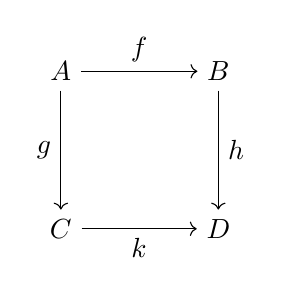
\begin{tikzpicture}
            \node (A) at (0,0) {\(A\)};
            \node (B) at (2,0) {\(B\)};
            \node (C) at (0,-2) {\(C\)};
            \node (D) at (2,-2) {\(D\)};
            \draw[->] (A) -- node[above] {\(f\)} (B);
            \draw[->] (A) -- node[left] {\(g\)} (C);
            \draw[->] (B) -- node[right] {\(h\)} (D);
            \draw[->] (C) -- node[below] {\(k\)} (D);
        \end{tikzpicture}
    \end{center}
    图表交换意味着两点间任意态射合成均相等, 比如 \(h \circ f = k \circ g\).
\end{definition}

\begin{example}
    定义 \(\mathbf{Set}\) 为集合范畴, 其中对象为集合, 对象间态射为映射.
\end{example}

\begin{example}
    定义 \(\mathbf{0}\) 为空范畴, 也即 \(\mathrm{Ob} (\mathbf{0}) = \emptyset\).
\end{example}

\begin{example}
    对偏序集 \(P\), 定义其对应的范畴 \(\mathrm{Cat} (P)\) 如下:

    \begin{enumerate}
        \item 对象是 \(P\) 中的元素.
        \item \(x \leq y\) 时有唯一态射 \(x \to y\).
        \item \(x \nleq y\) 时没有态射.
    \end{enumerate}
\end{example}

\begin{definition}
    对集合 \(S\) 定义离散范畴 \(\mathrm{Disc} (S)\) 如下:

    \begin{enumerate}
        \item 对象是 \(S\) 中的元素.
        \item 仅有单位态射.
    \end{enumerate}
\end{definition}

\begin{definition}
    若有一组映射 \(f : X \to Y\), \(g : Y \to X\) 使得 \(g \circ f = \mathrm{id}_X\), \(f \circ g = \mathrm{id}_Y\), 则称 \(f\) 为 \(g\) 的逆, \(f\) 是同构,
    记作 \(f^{-1} = g\).

    \(X\) 与 \(Y\) 同构记作 \(X \cong Y\), 命全体 \(X\) 与 \(Y\) 间的同构为 \(\mathrm{Isom}_{\mathcal{C}} (X,Y)\).
\end{definition}

\begin{definition}
    定义自同态集 \(\mathrm{End}_{\mathcal{C}} (X) := \mathrm{Hom}_{\mathcal{C}} (X,X)\) 与自同构集
    \(\mathrm{Aut}_{\mathcal{C}} (X) := \mathrm{Isom}_{\mathcal{C}} (X,X)\), 其上有自然的复合运算.
\end{definition}

\begin{definition}
    态射 \(f : X \to Y\) 称为单态射 (monomorphism), 如果对于任意 \(g,h : Z \to X\), 有 \(f \circ g = f \circ h \implies g = h\).

    态射 \(f : X \to Y\) 称为满态射 (epimorphism), 如果对于任意 \(g,h : Y \to Z\), 有 \(g \circ f = h \circ f \implies g = h\).
\end{definition}

\begin{definition}[反范畴]
    定义范畴 \(\mathcal{C}^{\mathrm{op}}\) 如下:

    \begin{enumerate}
        \item \(\mathrm{Ob} (\mathcal{C}^{\mathrm{op}}) = \mathrm{Ob} (\mathcal{C})\).
        \item \(\mathrm{Hom}_{\mathcal{C}^{\mathrm{op}}} (X,Y) = \mathrm{Hom}_{\mathcal{C}} (Y,X)\).
        \item 对于态射 \(f : X \to Y, g : Y \to Z\), 定义 \(g \circ_{\mathrm{op}} f := f \circ g\).
    \end{enumerate}
\end{definition}

\begin{definition}[函子]
    \label {definition:functor}
    一个函子 \(F : \mathcal{C} \to \mathcal{D}\) 包含以下资料:

    \begin{enumerate}
        \item 对象映射 \(F : \mathrm{Ob} (\mathcal{C}) \to \mathrm{Ob} (\mathcal{D})\).
        \item 对于任意对象 \(X,Y \in \mathcal{C}\), 有映射 \(F : \mathrm{Hom}_{\mathcal{C}} (X,Y) \to \mathrm{Hom}_{\mathcal{D}} (F(X),F(Y))\).
        \item 对于任意对象 \(X \in \mathcal{C}\), 映单位态射为单位态射 \(F(\mathrm{id}_X) = \mathrm{id}_{F(X)}\).
        \item 对于任意对象 \(X,Y,Z \in \mathcal{C}\) 保持态射的复合 \(F(g \circ f) = F(g) \circ F(f)\).
    \end{enumerate}
\end{definition}

\begin{definition}[反变函子]
    定义 \(\mathcal{C}\) 出发反变函子为从其反范畴出发的函子.
\end{definition}

\begin{definition}
    一个函子称为忠实 (faithful), 如果对于任意对象 \(X,Y \in \mathcal{C}\), 映射 \(F : \mathrm{Hom}_{\mathcal{C}} (X,Y) \to \mathrm{Hom}_{\mathcal{D}} (F(X),F(Y))\) 是单射.

    一个函子称为全 (full), 如果对于任意对象 \(X,Y \in \mathcal{C}\), 映射 \(F : \mathrm{Hom}_{\mathcal{C}} (X,Y) \to \mathrm{Hom}_{\mathcal{D}} (F(X),F(Y))\) 是满射.

    一个函子称本质满 (essentially surjective), 如果对于任意对象 \(Y \in \mathcal{D}\), 存在对象 \(X \in \mathcal{C}\) 使得 \(F(X) \cong Y\).
\end{definition}

\begin{definition}
    对于函子 \(F : \mathcal{C} \to \mathcal{D}\), \(G : \mathcal{D} \to \mathcal{E}\), 定义函子间的复合 \((G \circ F) (X) := G(F(X))\), \((G \circ F) (f) := G(F(f))\).

    \begin{proof}
        只需注意到 \(G(F(f)) \circ G(F(g)) = G(F(f) \circ F(g)) = G(F(f \circ g))\).
    \end{proof}
\end{definition}

\begin{definition}
    显见函子复合满足结合律, 定义范畴 \(\mathbf{Cat}\) 如下:

    \begin{enumerate}
        \item 对象是 \(\mathrm{Ob} (\mathcal{C}), \mathrm{Mor} (\mathcal{C})\) 是集合的范畴 \(\mathcal{C}\).
        \item \(\mathrm{Hom}_{\mathbf{Cat}} (\mathcal{C},\mathcal{D})\) 是所有函子 \(\mathcal{C} \to \mathcal{D}\).
    \end{enumerate}
\end{definition}

\begin{definition}[自然变换]
    两个函子 \(F,G : \mathcal{C} \to \mathcal{D}\) 之间的自然变换 (natural transformation) \(\eta : F \to G\) 为对所有 \(X \in \mathrm{Ob} (C)\) 择定的态射 \(\eta_X : F(X) \to G(X)\),
    满足对于任意对象 \(X,Y \in \mathcal{C}\) 与 \(f \in \mathrm{Hom}_{\mathcal{C}} (X,Y)\), 有交换图表:
        
    \begin{center}
        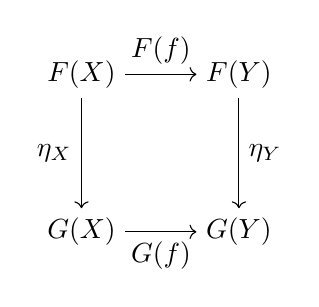
\begin{tikzpicture}
            \node (FX) at (0,0) {\(F(X)\)};
            \node (FY) at (2,0) {\(F(Y)\)};
            \node (GX) at (0,-2) {\(G(X)\)};
            \node (GY) at (2,-2) {\(G(Y)\)};
            \draw[->] (FX) -- node[above] {\(F(f)\)} (FY);
            \draw[->] (FX) -- node[left] {\(\eta_X\)} (GX);
            \draw[->] (FY) -- node[right] {\(\eta_Y\)} (GY);
            \draw[->] (GX) -- node[below] {\(G(f)\)} (GY);
        \end{tikzpicture}
    \end{center}

    记作 \(\eta : F \to G\), 可以画作图表:

    \begin{center}
        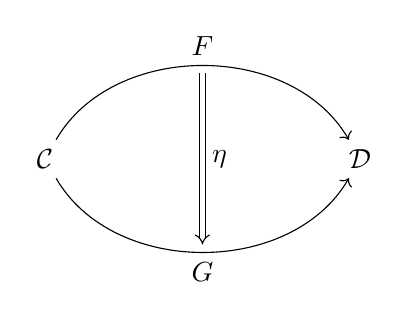
\begin{tikzpicture}
            \node (C) at (-2,0) {\(\mathcal{C}\)};
            \node (D) at (2,0) {\(\mathcal{D}\)};
            \draw[->] (C) to[bend left=60] node[above] (F) {\(F\)} (D);
            \draw[->] (C) to[bend right=60] node[below] (G) {\(G\)} (D);
            \draw[double,-{Implies},double distance = 0.15em] ($(F.south) + (0,- 0.1)$) to node[right] {\(\eta\)} ($(G.north) + (0,0.1)$);
        \end{tikzpicture}
    \end{center}
\end{definition}

\begin{definition}[纵合成]
    给出 \(\eta : F \to G\), \(\theta : G \to H\), 定义纵合成 \(\theta \circ \eta : F \to H\) 为 \({(\theta \circ \eta)}_X := \theta_X \circ \eta_X\), 解作图表:
    
    \[
        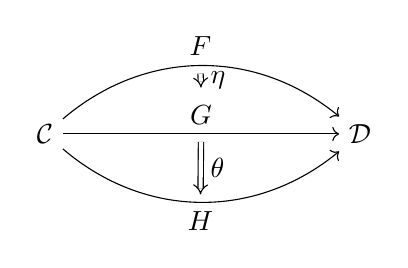
\begin{tikzpicture}
            \node (C) at (-2,0) {\(\mathcal{C}\)};
            \node (D) at (2,0) {\(\mathcal{D}\)};
            \draw[->] (C) to[bend left=40] node[above] (F) {\(F\)} (D);
            \draw[->] (C) to node[above] (G) {\(G\)} (D);
            \draw[->] (C) to[bend right=40] node[below] (H) {\(H\)} (D);
            \draw[double,-{Implies},double distance = 0.15em] ($(F.south) + (0,- 0.1)$) to node[right] {\(\eta\)} ($(G.north) + (0,0.1)$);
            \draw[double,-{Implies},double distance = 0.15em] ($(G.south) + (0,- 0.1)$) to node[right] {\(\theta\)} ($(H.north) + (0,0.1)$);
        \end{tikzpicture} = 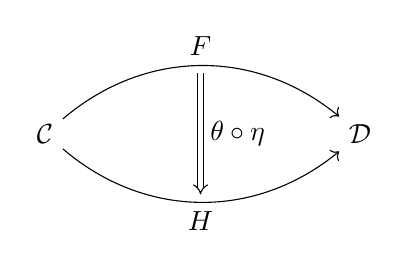
\begin{tikzpicture}
            \node (C) at (-2,0) {\(\mathcal{C}\)};
            \node (D) at (2,0) {\(\mathcal{D}\)};
            \draw[->] (C) to[bend left=40] node[above] (F) {\(F\)} (D);
            \draw[->] (C) to[bend right=40] node[below] (H) {\(H\)} (D);
            \draw[double,-{Implies},double distance = 0.15em] ($(F.south) + (0,- 0.1)$) to node[right] {\(\theta \circ \eta\)} ($(H.north) + (0,0.1)$);
        \end{tikzpicture}
    \]

    \begin{proof}
        只需注意到以下交换图表 (两小方块交换故外框交换):

        \begin{center}
            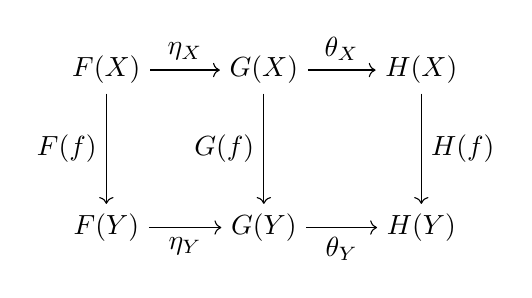
\begin{tikzpicture}
                \node (FX) at (-2,1) {\(F(X)\)};
                \node (FY) at (-2,-1) {\(F(Y)\)};
                \node (GX) at (0,1) {\(G(X)\)};
                \node (GY) at (0,-1) {\(G(Y)\)};
                \node (HX) at (2,1) {\(H(X)\)};
                \node (HY) at (2,-1) {\(H(Y)\)};
                \draw[->] (FX) -- node[left] {\(F(f)\)} (FY);
                \draw[->] (FX) -- node[above] {\(\eta_X\)} (GX);
                \draw[->] (FY) -- node[below] {\(\eta_Y\)} (GY);
                \draw[->] (GX) -- node[left] {\(G(f)\)} (GY);
                \draw[->] (GX) -- node[above] {\(\theta_X\)} (HX);
                \draw[->] (GY) -- node[below] {\(\theta_Y\)} (HY);
                \draw[->] (HX) -- node[right] {\(H(f)\)} (HY);
            \end{tikzpicture}
        \end{center}
    \end{proof}
\end{definition}

\begin{definition}[横合成]
    给出三个范畴 \(\mathcal{C},\mathcal{D},\mathcal{E}\) 以及四个函子 \(F_1,F_2 : \mathcal{C} \to \mathcal{D}\), \(G_1,G_2 : \mathcal{D} \to \mathcal{E}\), 
    给出自然变换 \(\eta : F_1 \to F_2\), \(\theta : G_1 \to G_2\), 定义横合成 \(\theta \ast \eta : G_1 \circ F_1 \to G_2 \circ F_2\) 为 \({(\theta \ast \eta)}_X := \theta_{F_2 (X)} \circ G_1 (\eta_X)\), 解作图表:

    \[
        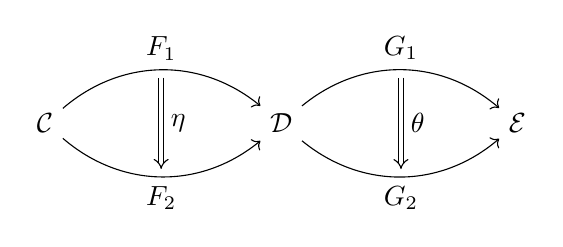
\begin{tikzpicture}
            \node (C) at (-3,0) {\(\mathcal{C}\)};
            \node (D) at (0,0) {\(\mathcal{D}\)};
            \node (E) at (3,0) {\(\mathcal{E}\)};
            \draw[->] (C) to[bend left=40] node[above] (F1) {\(F_1\)} (D);
            \draw[->] (C) to[bend right=40] node[below] (F2) {\(F_2\)} (D);
            \draw[->] (D) to[bend left=40] node[above] (G1) {\(G_1\)} (E);
            \draw[->] (D) to[bend right=40] node[below] (G2) {\(G_2\)} (E);
            \draw[double,-{Implies},double distance = 0.15em] ($(F1.south) + (0,- 0.1)$) to node[right] {\(\eta\)} ($(F2.north) + (0,0.1)$);
            \draw[double,-{Implies},double distance = 0.15em] ($(G1.south) + (0,- 0.1)$) to node[right] {\(\theta\)} ($(G2.north) + (0,0.1)$);
        \end{tikzpicture} = 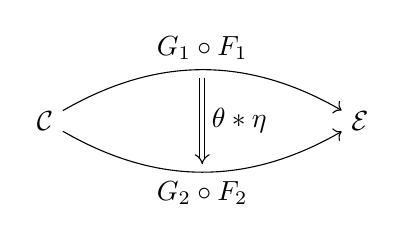
\begin{tikzpicture}
            \node (C) at (-2,0) {\(\mathcal{C}\)};
            \node (E) at (2,0) {\(\mathcal{E}\)};
            \draw[->] (C) to[bend left=30] node[above] (G1F1) {\(G_1 \circ F_1\)} (E);
            \draw[->] (C) to[bend right=30] node[below] (G2F2) {\(G_2 \circ F_2\)} (E);
            \draw[double,-{Implies},double distance = 0.15em] ($(G1F1.south) + (0,- 0.1)$) to node[right] {\(\theta \ast \eta\)} ($(G2F2.north) + (0,0.1)$);
        \end{tikzpicture}
    \]

    \begin{proof}
        需注意到以下交换图表:

        \begin{center}
            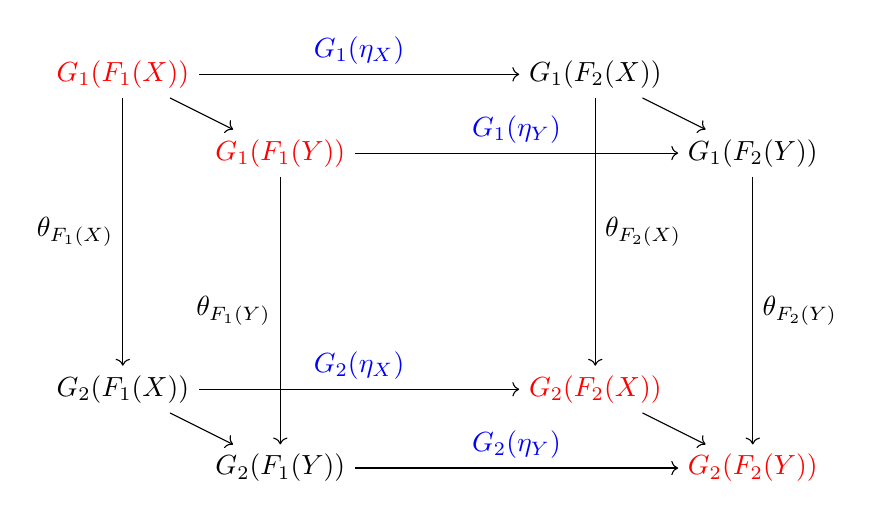
\begin{tikzpicture}
                \node (G1F1X) at (-4,4) {\textcolor{red}{\(G_1 (F_1 (X))\)}};
                \node (G1F1Y) at (-2,3) {\textcolor{red}{\(G_1 (F_1 (Y))\)}};
                \node (G1F2X) at (2,4) {\(G_1 (F_2 (X))\)};
                \node (G1F2Y) at (4,3) {\(G_1 (F_2 (Y))\)};
                \node (G2F1X) at (-4,0) {\(G_2 (F_1 (X))\)};
                \node (G2F1Y) at (-2,-1) {\(G_2 (F_1 (Y))\)};
                \node (G2F2X) at (2,0) {\textcolor{red}{\(G_2 (F_2 (X))\)}};
                \node (G2F2Y) at (4,-1) {\textcolor{red}{\(G_2 (F_2 (Y))\)}};
                \draw[->] (G1F1X) -- (G1F1Y);
                \draw[->] (G1F2X) -- (G1F2Y);
                \draw[->] (G2F1X) -- (G2F1Y);
                \draw[->] (G2F2X) -- (G2F2Y);
                \draw[->] (G1F1X) -- node[above] {\textcolor{blue}{\(G_1 (\eta_X)\)}} (G1F2X);
                \draw[->] (G1F1Y) -- node[above] {\textcolor{blue}{\(G_1 (\eta_Y)\)}} (G1F2Y);
                \draw[->] (G2F1X) -- node[above] {\textcolor{blue}{\(G_2 (\eta_X)\)}} (G2F2X);
                \draw[->] (G2F1Y) -- node[above] {\textcolor{blue}{\(G_2 (\eta_Y)\)}} (G2F2Y);
                \draw[->] (G1F1X) -- node[left] {{\(\theta_{F_1 (X)}\)}} (G2F1X);
                \draw[->] (G1F1Y) -- node[left] {\(\theta_{F_1 (Y)}\)} (G2F1Y);
                \draw[->] (G1F2X) -- node[right] {\(\theta_{F_2 (X)}\)} (G2F2X);
                \draw[->] (G1F2Y) -- node[right] {\(\theta_{F_2 (Y)}\)} (G2F2Y);
            \end{tikzpicture}
        \end{center}

        前后左右四面交换源自 \(\theta\) 为自然变换, 上下两面交换源自 \(\eta\) 为自然变换, 于是\textcolor{red}{红色}标记出的子图亦交换.
    \end{proof}
\end{definition}

特别的, 在标记自然变换时, 我们可以将单独的函子 \(F\) 拉开成为 \(\mathrm{id}_F : F \to F\), 在每个 \(X\) 上为 \(\mathrm{id}_{F(X)}\).

\begin{definition}
    对于范畴 \(\mathcal{C}, \mathcal{D}\), 定义函子范畴 \(\mathbf{Fun} (\mathcal{C},\mathcal{D})\) 如下:

    \begin{enumerate}
        \item 对象是函子 \(\mathcal{C} \to \mathcal{D}\).
        \item 对于函子 \(F,G : \mathcal{C} \to \mathcal{D}\), 定义态射集 \(\mathrm{Hom}_{\mathbf{Fun} (\mathcal{C},\mathcal{D})} (F,G)\) 为所有 \(F \to G\) 的自然变换.
        \item 态射的合成是自然变换的纵合成.
    \end{enumerate}

    \begin{proof}
        只需证明纵合成之结合律, 只需注意到态射结合律:

        \[
            (\theta_X \circ \eta_X) \circ \phi_X = \theta_X \circ (\eta_X \circ \phi_X)
        \]
    \end{proof}
\end{definition}

\begin{lemma}
    函子的纵合成满足结合律.

    \begin{proof}
        给出自然变换 \(\theta, \psi, \phi\) 如下:

        \begin{center}
            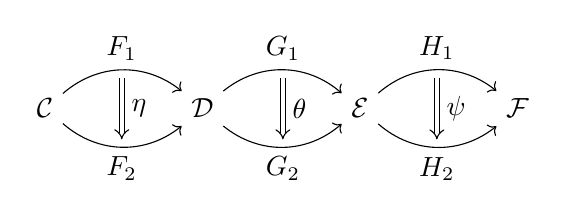
\begin{tikzpicture}
                \node (C) at (-3,0) {\(\mathcal{C}\)};
                \node (D) at (-1,0) {\(\mathcal{D}\)};
                \node (E) at (1,0) {\(\mathcal{E}\)};
                \node (F) at (3,0) {\(\mathcal{F}\)};
                \draw[->] (C) to[bend left=40] node[above] (F1) {\(F_1\)} (D);
                \draw[->] (C) to[bend right=40] node[below] (F2) {\(F_2\)} (D);
                \draw[->] (D) to[bend left=40] node[above] (G1) {\(G_1\)} (E);
                \draw[->] (D) to[bend right=40] node[below] (G2) {\(G_2\)} (E);
                \draw[->] (E) to[bend left=40] node[above] (H1) {\(H_1\)} (F);
                \draw[->] (E) to[bend right=40] node[below] (H2) {\(H_2\)} (F);
                \draw[double,-{Implies},double distance = 0.15em] ($(F1.south) + (0,- 0.1)$) to node[right] {\(\eta\)} ($(F2.north) + (0,0.1)$);
                \draw[double,-{Implies},double distance = 0.15em] ($(G1.south) + (0,- 0.1)$) to node[right] {\(\theta\)} ($(G2.north) + (0,0.1)$);
                \draw[double,-{Implies},double distance = 0.15em] ($(H1.south) + (0,- 0.1)$) to node[right] {\(\psi\)} ($(H2.north) + (0,0.1)$);
            \end{tikzpicture}
        \end{center}

        有交换图表 (交换性源自于施 \(\psi\) 自然性于 \(G_2 \eta_X\)):

        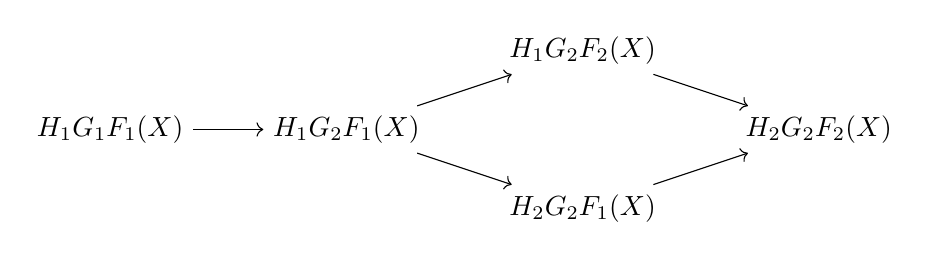
\begin{tikzpicture}
            \node (H1G1F1) at (-4.5,0) {\(H_1 G_1 F_1 (X)\)};
            \node (H1G2F1) at (-1.5,0) {\(H_1 G_2 F_1 (X)\)};
            \node (H1G2F2) at (1.5,1) {\(H_1 G_2 F_2 (X)\)};
            \node (H2G2F2) at (4.5,0) {\(H_2 G_2 F_2 (X)\)};
            \node (H2G2F1) at (1.5,-1) {\(H_2 G_2 F_1 (X)\)};
            \draw[->] (H1G1F1) -- (H1G2F1);
            \draw[->] (H1G2F1) -- (H1G2F2);
            \draw[->] (H1G2F2) -- (H2G2F2);
            \draw[->] (H1G2F1) -- (H2G2F1);
            \draw[->] (H2G2F1) -- (H2G2F2);
        \end{tikzpicture}
    \end{proof}
\end{lemma}

\begin{lemma}
    函子的横纵合成交换, 即亦给出自然变换如下:

    \begin{center}
        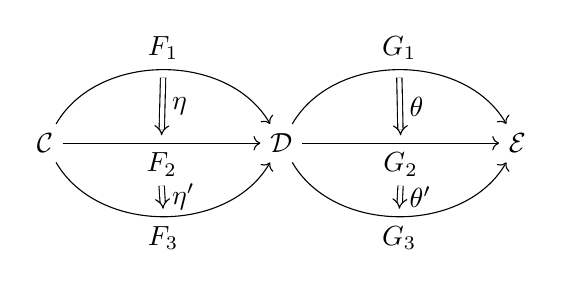
\begin{tikzpicture}
            \node (C) at (-3,0) {\(\mathcal{C}\)};
            \node (D) at (0,0) {\(\mathcal{D}\)};
            \node (E) at (3,0) {\(\mathcal{E}\)};
            \draw[->] (C) to[bend left=60] node[above] (F1) {\(F_1\)} (D);
            \draw[->] (C) to node[below] (F2) {\(F_2\)} (D);
            \draw[->] (C) to[bend right=60] node[below] (F3) {\(F_3\)} (D);
            \draw[->] (D) to[bend left=60] node[above] (G1) {\(G_1\)} (E);
            \draw[->] (D) to node[below] (G2) {\(G_2\)} (E);
            \draw[->] (D) to[bend right=60] node[below] (G3) {\(G_3\)} (E);
            \draw[double,-{Implies},double distance = 0.15em] ($(F1.south) + (0,- 0.1)$) to node[right] {\(\eta\)} ($(F2.north) + (0,0.1)$);
            \draw[double,-{Implies},double distance = 0.15em] ($(F2.south)$) to node[right] {\(\eta^\prime\)} ($(F3.north) + (0,0.1)$);
            \draw[double,-{Implies},double distance = 0.15em] ($(G1.south) + (0,- 0.1)$) to node[right] {\(\theta\)} ($(G2.north) + (0,0.1)$);
            \draw[double,-{Implies},double distance = 0.15em] ($(G2.south)$) to node[right] {\(\theta^\prime\)} ($(G3.north) + (0,0.1)$);
        \end{tikzpicture}
    \end{center}

    则有等式 \((\theta^\prime \ast \eta^\prime) \circ (\theta \ast \eta) = (\theta^\prime \circ \theta) \ast (\eta^\prime \circ \eta)\).

    \begin{proof}
        只需注意到以下交换图表:

        \begin{center}
            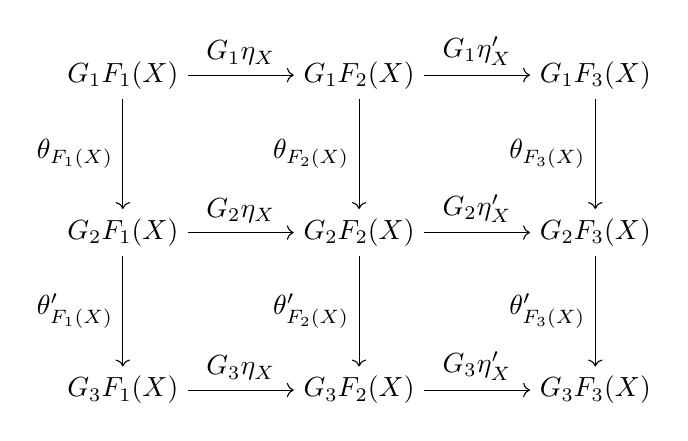
\begin{tikzpicture}
                \node (G1F1X) at (-3,2) {\(G_1 F_1 (X)\)};
                \node (G1F2X) at (0,2) {\(G_1 F_2 (X)\)};
                \node (G1F3X) at (3,2) {\(G_1 F_3 (X)\)};
                \node (G2F1X) at (-3,0) {\(G_2 F_1 (X)\)};
                \node (G2F2X) at (0,0) {\(G_2 F_2 (X)\)};
                \node (G2F3X) at (3,0) {\(G_2 F_3 (X)\)};
                \node (G3F1X) at (-3,-2) {\(G_3 F_1 (X)\)};
                \node (G3F2X) at (0,-2) {\(G_3 F_2 (X)\)};
                \node (G3F3X) at (3,-2) {\(G_3 F_3 (X)\)};
                \draw[->] (G1F1X) to node[above] {\(G_1 \eta_X\)} (G1F2X);
                \draw[->] (G1F2X) to node[above] {\(G_1 \eta^\prime_X\)} (G1F3X);
                \draw[->] (G2F1X) to node[above] {\(G_2 \eta_X\)} (G2F2X);
                \draw[->] (G2F2X) to node[above] {\(G_2 \eta^\prime_X\)} (G2F3X);
                \draw[->] (G3F1X) to node[above] {\(G_3 \eta_X\)} (G3F2X);
                \draw[->] (G3F2X) to node[above] {\(G_3 \eta^\prime_X\)} (G3F3X);
                \draw[->] (G1F1X) to node[left] {\(\theta_{F_1 (X)}\)} (G2F1X);
                \draw[->] (G1F2X) to node[left] {\(\theta_{F_2 (X)}\)} (G2F2X);
                \draw[->] (G1F3X) to node[left] {\(\theta_{F_3 (X)}\)} (G2F3X);
                \draw[->] (G2F1X) to node[left] {\(\theta^\prime_{F_1 (X)}\)} (G3F1X);
                \draw[->] (G2F2X) to node[left] {\(\theta^\prime_{F_2 (X)}\)} (G3F2X);
                \draw[->] (G2F3X) to node[left] {\(\theta^\prime_{F_3 (X)}\)} (G3F3X);
            \end{tikzpicture}
        \end{center}

        每个小正方形交换源于 \(\theta, \theta^\prime\) 为自然变换, 故外框交换.
    \end{proof}
\end{lemma}

\begin{lemma}
    \label {lemma:natural transformation is isomorphism iff each component is isomorphism}
    自然变换 \(\eta : F \to G\) 是同构当且仅当对于任意 \(X \in \mathcal{C}\), \(\eta_X\) 是同构,
    其逆为 \(\eta^{-1} : G \to F\), \(\eta^{-1}_X := {\eta_X}^{-1}\).

    \begin{proof}
        给出其逆业已给出每个 \(\eta_X\) 之逆, 而 \(\eta^{-1}\) 是自然性对应了
        \(\eta\) 自然性的交换图表, 换言之, 以下图表每一小块交换故外框交换.

        \begin{center}
            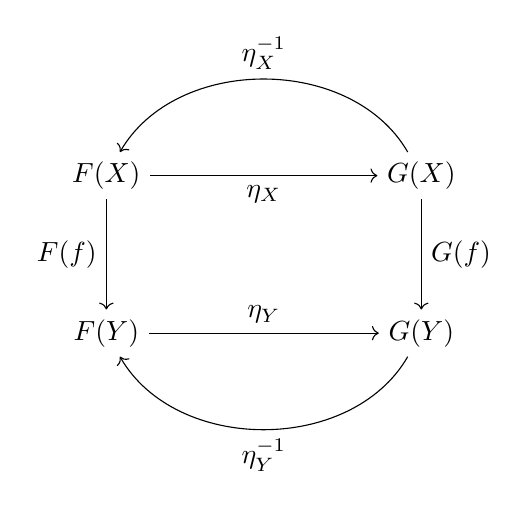
\begin{tikzpicture}
                \node (FX) at (-2,1) {\(F(X)\)};
                \node (FY) at (-2,-1) {\(F(Y)\)};
                \node (GX) at (2,1) {\(G(X)\)};
                \node (GY) at (2,-1) {\(G(Y)\)};
                \draw[->] (FX) to node[left] {\(F(f)\)} (FY);
                \draw[->] (FX) to node[below] {\(\eta_X\)} (GX);
                \draw[->] (FY) to node[above] {\(\eta_Y\)} (GY);
                \draw[->] (GX) to node[right] {\(G(f)\)} (GY);
                \draw[->] (GX) to [bend right=60] node[above] {\(\eta^{-1}_X\)} (FX);
                \draw[->] (GY) to [bend left=60] node[below] {\(\eta^{-1}_Y\)} (FY);
            \end{tikzpicture}
        \end{center}
    \end{proof}
\end{lemma}

\begin{definition}[范畴等价]
    若存在函子 \(F : \mathcal{C} \to \mathcal{D}\), \(G : \mathcal{D} \to \mathcal{C}\) 使得 \(G \circ F \cong \mathrm{id}_{\mathcal{C}}\), \(F \circ G \cong \mathrm{id}_{\mathcal{D}}\), 则称 \(\mathcal{C}\) 与 \(\mathcal{D}\) 等价.

    假定上述定义中 \(\cong\) 为 \(=\), 则称 \(\mathcal{C}\) 与 \(\mathcal{D}\) 同构.
\end{definition}

\begin{definition}[子范畴]
    给定范畴 \(\mathcal{C}^\prime, \mathcal{C}\), 若 \(\mathrm{Ob} (\mathcal{C}^\prime) \subseteq \mathrm{Ob} (\mathcal{C})\), 
    \(\mathrm{Hom}_{\mathcal{C}^\prime} (X,Y) \subseteq \mathrm{Hom}_{\mathcal{C}} (X,Y)\), 且保持复合运算,
    则称 \(\mathcal{C}^\prime\) 是 \(\mathcal{C}\) 的子范畴 (subcategory), 子范畴对应一个自然的嵌入 \(\iota : \mathcal{C}^\prime \to \mathcal{C}\),
    总是忠实, 子范畴亦有全和本质满的性质.
\end{definition}

\begin{definition}[骨架]
    如果范畴 \(\mathcal{C}^\prime\) 是 \(\mathcal{C}\) 的全子范畴, 且对于任意 \(X \in \mathrm{Ob} (\mathcal{C})\),
    都存在唯一 \(X^\prime \in \mathrm{Ob} (\mathcal{C}^\prime)\) 使得 \(X \cong X^\prime\), 则称 \(\mathcal{C}^\prime\) 是 \(\mathcal{C}\) 的骨架 (skeleton).

    自身是骨架的范畴称为骨架范畴 (skeletal category).
\end{definition}

\begin{definition}[小范畴]
    为了避免一些集合论的困难, 我们定义小范畴 (small category) 为态射类是集合的范畴.

    给出一个 Grothendieck 宇宙 \(\mathcal{U}\), 定义 \(\mathcal{U}\)-小范畴为对象类是 \(\mathcal{U}\) 中的集合的范畴.
\end{definition}

\begin{lemma}
    任何小范畴 \(\mathcal{C}\) 有骨架, 且骨架范畴与 \(\mathcal{C}\) 等价.

    \begin{proof}
        注意到 \(\cong\) 显见的是 \(\mathrm{Ob} (\mathcal{C})\) 上的等价关系, 在每个等价类
        上使用 \ref{axiom:NBG Axiom of Choice} 选取代表元 \(X^\prime\), 与等价类中任意一 \(X\) 与 \(X^\prime\) 间同构 \(f_X : X \to X^\prime\),
        选取子范畴 \(\mathcal{C}^\prime\) 如下:

        \begin{enumerate}
            \item 对象集为全体代表元 \(X^\prime\).
            \item 对于任意 \(X^\prime,Y^\prime \in \mathrm{Ob} (\mathcal{C}^\prime)\), \(\mathrm{Hom}_{\mathcal{C}^\prime} (X^\prime,Y^\prime) = \mathrm{Hom}_{\mathcal{C}} (X^\prime,Y^\prime) \).
        \end{enumerate}

        定义 \(\iota^{-1}\) 映 \(X\) 为其代表元 \(X^\prime\), 映 \(f \in \mathrm{Hom}_{\mathcal{C}} (X,Y)\) 为 
        \(f_Y \circ f \circ {f_X}^{-1}\).

        \(\iota^{-1}\) 函子性, \(\iota \circ \iota^{-1} = \mathrm{id}_{\mathcal{C}}\) 是显然的, 而构造 \(\iota^{-1} \circ \iota \cong \mathrm{id}_{\mathcal{C}^\prime}\) 的自然变换为 \(f\) 即可.
    \end{proof}
\end{lemma}

\begin{lemma}
    范畴等价具有传递性.

    \begin{proof}
        给出范畴 \(\mathcal{C},\mathcal{D},\mathcal{E}\), 函子 \(F : \mathcal{C} \to \mathcal{D}\), \(G : \mathcal{D} \to \mathcal{E}\), 
        以及其逆, 给出可逆的自然变换 \(\eta : F \circ F^{-1} \to \mathrm{id}_{\mathcal{D}}\), \(\theta : F^{-1} \circ F \to \mathrm{id}_{\mathcal{C}}\),
        \(\eta^\prime : G \circ G^{-1} \to \mathrm{id}_{\mathcal{E}}\), \(\theta^\prime : G^{-1} \circ G \to \mathrm{id}_{\mathcal{D}}\), 构造自然变换
        \(\eta^\prime \circ (\mathrm{id}_G \ast \eta \ast \mathrm{id}_{G^{-1}}) : G \circ F \circ F^{-1} \circ G^{-1} \to \mathrm{id}_{\mathcal{E}}\) 有逆
        \((\mathrm{id}_G \ast \eta^{-1} \ast \mathrm{id}_{G^{-1}}) \circ {\eta^{\prime}}^{-1}\),  \(\theta\) 侧可同理构造.
    \end{proof}
\end{lemma}

\begin{lemma}
    骨架范畴间的全忠实本质满函子都是同构.

    \begin{proof}
        本质满则在对象集上是双射, 全忠实亦给出每个态射集上的双射.
    \end{proof}
\end{lemma}

\begin{lemma}
    小范畴间函子 \(F\) 是等价当且仅当 \(F\) 全忠实本质满.

    \begin{proof}
        易得骨架范畴间的同构, 考虑等价的传递性即可.
    \end{proof}
\end{lemma}

\subsection{Hom 函子与泛性质}

\begin{definition}
    对于集合 \(I\) 与小范畴 \({(\mathcal{C}_i)}_{i \in I}\), 定义积范畴 \(\prod_{i \in I} \mathcal{C}_i\) 如下:

    \begin{enumerate}
        \item 对象是积 \(\prod_{i \in I} \mathrm{Ob} (\mathcal{C}_i)\) 的元素.
        \item 对于对象 \((X_i)_{i \in I}\), \((Y_i)_{i \in I}\), 定义态射集 \(\mathrm{Hom}_{\prod_{i \in I} \mathcal{C}_i} ((X_i)_{i \in I},(Y_i)_{i \in I})\) 为态射集之积
                \(\prod_{i \in I} \mathrm{Hom}_{\mathcal{C}_i} (X_i,Y_i)\).
        \item 态射的合成是逐点的, 也即 \({(f_i)}_{i \in I} \circ {(g_i)}_{i \in I} = {(f_i \circ g_i)}_{i \in I}\).
    \end{enumerate}

    定义余积范畴 \(\coprod_{i \in I} \mathcal{C}_i\) 如下:

    \begin{enumerate}
        \item 对象是无交并 \(\coprod_{i \in I} \mathrm{Ob} (\mathcal{C}_i)\) 的元素.
        \item 对象 \(X,Y\) 间有态射当且仅当其对应同一个 \(\mathcal{C}_i\), 态射集继承自 \(\mathcal{C}_i\).
    \end{enumerate}

    定义自明的投影函子 \(\mathbf{Pr}_j : \prod_{i \in I} \mathcal{C}_i \to \mathcal{C}_j\) 与包含函子 \(\mathbf{In}_j : \mathcal{C}_j \to \coprod_{i \in I} \mathcal{C}_i\).
\end{definition}

\begin{definition}
    多元函子即为从积范畴出发的函子.
\end{definition}

\begin{definition}[Hom 函子]
    对于任意范畴 \(\mathcal{C}\), 有函子 \(\mathrm{Hom}_{\mathcal{C}} (-,-) : \mathcal{C}^{\mathrm{op}} \times \mathcal{C} \to \mathbf{Set}\), 映 \((X,Y)\) 为态射集 \(\mathrm{Hom}_{\mathcal{C}} (X,Y)\), 
    映 \(\mathcal{C}^{\mathrm{op}} \times \mathcal{C}\) 中态射 \((f,g)\) 为映射 \(\phi \mapsto g \circ \phi \circ f\).

    称 \(\phi\) 对 \(f\) 做拉回 (pullback), 对 \(g\) 做推出 (pushforward).
\end{definition}

\begin{lemma}
    存在自然同构 \({(\mathbf{Fun} (\mathcal{C}_1 ,\mathcal{C}_2))}^\mathrm{op} \cong \mathbf{Fun} ({\mathcal{C}_1}^\mathrm{op}, {\mathcal{C}_2}^\mathrm{op})\).
\end{lemma}

\begin{lemma}
    有恒等式 \(\mathbf{Fun} (\mathrm{Disc} (I), \mathcal{C}) \cong \prod_{i \in I} \mathcal{C}\).
\end{lemma}

\begin{definition}[中心]
    一个范畴的中心定义为 \(\mathrm{Z} (\mathcal{C}) := \mathrm{End} (\mathrm{id}_{\mathcal{C}})\).

    对范畴等价 \(F : \mathcal{C} \to \mathcal{D}\), 诱导出中心的同构 \(\mathrm{Z} (\mathcal{C}) \cong \mathrm{Z} (\mathcal{D})\).
\end{definition}

\begin{definition}
    假设范畴 \(\mathcal{C}\) 中对象 \(X\) 满足任意 \(Y \in \mathrm{Ob} (\mathcal{C})\), \(\mathrm{Hom}_{\mathcal{C}} (X,Y)\) 是单点集, 则称 \(X\) 是始对象 (initial object).
    对称的 \(\mathrm{Hom}_{\mathcal{C}} (Y,X)\) 是单点集的对象称为终对象 (terminal object).既是始对象又是终对象的对象称为零对象 (zero object).
\end{definition}

\begin{example}
    在 \(\mathbf{Set}\) 中, 空集是始对象, 任意单点集是终对象.
\end{example}

\begin{definition}
    始对象间有唯一的同构, 终对象亦然.

    \begin{proof}
        给出始对象 \(X,Y\), 存在唯一的 \(f : X \to Y\), \(g : Y \to X\),
        同样存在唯一的 \(\mathrm{id}_X : X \to X\), \(\mathrm{id}_Y : Y \to Y\), 于是 \(f \circ g = \mathrm{id}_Y\), \(g \circ f = \mathrm{id}_X\).

        终对象只需注意到任意 \(\mathcal{C}\) 的终对象都是 \(\mathcal{C}^{\mathrm{op}}\) 的始对象.
    \end{proof}
\end{definition}

\begin{definition}
    泛性质 (universal property) 是一种在某个范畴下是始对象或终对象的性质, 其有自然的唯一性.
\end{definition}

\begin{definition}[图范畴]
    给出一个图表样式, 定义该图的范畴如下:

    \begin{enumerate}
        \item 对象是所有使得图表交换的一种填涂方式.
        \item 态射是相同位置的对象逐点的态射, 满足生成的柱状图表交换.
    \end{enumerate}
\end{definition}

\begin{example}[态射范畴]
    称下图的图范畴为 \(\mathcal{C}\) 的态射范畴:

    \begin{center}
        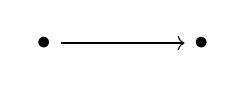
\begin{tikzpicture}
            \node (P1) at (-1,0) {\(\bullet\)};
            \node (P2) at (1,0) {\(\bullet\)};
            \draw[->] (P1) to (P2);
        \end{tikzpicture}
    \end{center}

    即对象是 \(\mathcal{C}\) 中两个对象 \(A,B\) 和一个态射 \(f : A \to B\), 由于确定 \(f\) 亦确定了 \(A,B\),
    也可将对象解作 \(\mathcal{C}\) 中的映射, \(f_1,f_2\) 间的态射是满足以下图表交换的 \((\phi_A, \phi_B)\):

    \begin{center}
        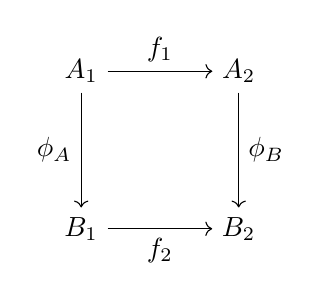
\begin{tikzpicture}
            \node (A1) at (-1,1) {\(A_1\)};
            \node (A2) at (1,1) {\(A_2\)};
            \node (B1) at (-1,-1) {\(B_1\)};
            \node (B2) at (1,-1) {\(B_2\)};
            \draw[->] (A1) to node[above] {\(f_1\)} (A2);
            \draw[->] (B1) to node[below] {\(f_2\)} (B2);
            \draw[->] (A1) to node[left] {\(\phi_A\)} (B1);
            \draw[->] (A2) to node[right] {\(\phi_B\)} (B2);
        \end{tikzpicture}
    \end{center}
\end{example}

\begin{example}[逗号范畴]
    给出函子 \(S : \mathcal{A} \to \mathcal{C}\), \(T : \mathcal{B} \to \mathcal{C}\), 定义逗号范畴 \((S / T)\) 为下图的图范畴:

    \begin{center}
        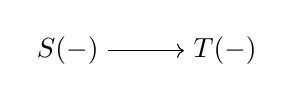
\begin{tikzpicture}
            \node (S) at (-1,0) {\(S (-)\)};
            \node (T) at (1,0) {\(T (-)\)};
            \draw[->] (S) to (T);
        \end{tikzpicture}
    \end{center}

    解作对象是 \(\mathcal{A}\) 中的对象 \(A\), \(\mathcal{B}\) 中的对象 \(B\), 以及 \(\mathcal{C}\) 中的态射 \(f : S(A) \to T(B)\) 组成的 \((A,B,f)\),
    一个 \((A,B,f)\) 到 \((A^\prime,B^\prime,f^\prime)\) 的态射是一对态射 \(g : A \to A^\prime\) 与 \(h : B \to B^\prime\) 使得下图交换:

    \begin{center}
        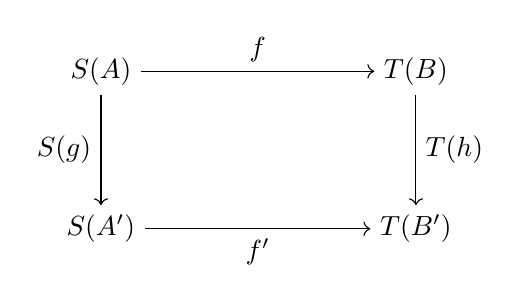
\begin{tikzpicture}
            \node (SA) at (-2,1) {\(S(A)\)};
            \node (TB) at (2,1) {\(T(B)\)};
            \node (SAP) at (-2,-1) {\(S(A^\prime)\)};
            \node (TBP) at (2,-1) {\(T(B^\prime)\)};
            \draw[->] (SA) to node[above] {\(f\)} (TB);
            \draw[->] (SAP) to node[below] {\(f^\prime\)} (TBP);
            \draw[->] (SA) to node[left] {\(S(g)\)} (SAP);
            \draw[->] (TB) to node[right] {\(T(h)\)} (TBP);
        \end{tikzpicture}
    \end{center}
\end{example}

\begin{definition}[子对象, 商对象]
    对 \(X \in \mathrm{Ob} (\mathcal{C})\), 定义 \(X\) 的子对象为单态射 \(i : Y \to X\),
    定义商对象为满态射 \(p : X \to Z\), 在子对象和商对象上定义序:

    定义子对象与商对象的范畴:

    \begin{enumerate}
        \item 对象是 \(X\) 的子对象.
        \item \(i_1 : Y_1 \to X\) 与 \(i_2 : Y_2 \to X\) 的态射是 \(f : Y_1 \to Y_2\) 使得 \(i_1 = i_2 \circ f\).
    \end{enumerate}

    \begin{enumerate}
        \item 对象是 \(X\) 的商对象.
        \item \(p_1 : X \to Z_1\) 与 \(p_2 : X \to Z_2\) 的态射是 \(f : Z_1 \to Z_2\) 使得 \(p_1 = f \circ p_2\).
    \end{enumerate}

    定义子对象与商对象的偏序: \(i_1 \le i_2\) 当且仅当有子对象范畴中的态射 \(f : Y_1 \to Y_2\),
    \(p_1 \le p_2\) 当且仅当有商对象范畴中的态射 \(f : Z_1 \to Z_2\).
\end{definition}

\begin{lemma}
    如果子对象 \(i_1 \le i_2\) 且 \(i_2 \le i_1\), 则子对象 \(i_1\) 与 \(i_2\) 同构, 商对象亦然.

    \begin{proof}
        注意到两个子对象间存在态射则唯一, 于是两个方向均合成为恒等态射.

        商对象无非是 \(\mathcal{C}^{\mathrm{op}}\) 中的子对象.
    \end{proof}
\end{lemma}

\subsection{米田引理}

\begin{definition}[预层]
    给出小范畴 \(\mathcal{C}\), 定义范畴 \(\mathcal{C}^{\vee} : \mathbf{Fun} (\mathcal{C}^{\mathrm{op}}, \mathbf{Set}^{\mathrm{op}})\) 与
    \(\mathcal{C}^{\wedge} : \mathbf{Fun} (\mathcal{C}^{\mathrm{op}}, \mathbf{Set})\), 称 \(\mathcal{C}^{\wedge}\) 为预层 (presheaf) 范畴.
\end{definition}

\begin{definition}
    我们可以自然的将 \(\mathcal{C}\) 嵌入 \(\mathcal{C}^{\wedge}\) 如下:
    \[
        h_{\mathcal{C}} : S \mapsto \mathrm{Hom}_{\mathcal{C}} (-,S)
    \]
    定义自然的求值函子 \(\mathrm{ev}^{\wedge} : \mathcal{C}^{\mathrm{op}} \times \mathcal{C}^{\wedge} \to \mathbf{Set}\) 如下:
    \[
        \mathrm{ev}^{\wedge} (X,S) := S(X)
    \]
    对偶的, 定义 \(k_\mathcal{C} : \mathcal{C} \to \mathcal{C}^{\vee}, \mathrm{ev}^{\vee} : {(\mathcal{C}^{\vee})}^{\mathrm{op}} \times \mathcal{C} \to \mathbf{Set}\) 如下:
    \[
        k_\mathcal{C} (S) := \mathrm{Hom}_{\mathcal{C}} (S,-), \mathrm{ev}^{\vee} (S,X) := S(X)
    \]
\end{definition}

下述引理称米田引理 (Yoneda lemma), 是范畴论中非常重要的引理.

\begin{lemma}[Yoneda]
    \setlabel {米田引理}
    \label {lemma:Yoneda lemma}
    对于任意 \(\mathcal{C}\) 上的预层 \(A \in \mathrm{Ob} (\mathcal{C}^{\wedge})\), 与对象 \(S \in \mathcal{C}\), 
    存在 \(\mathrm{Hom}_{\mathcal{C}^{\wedge}} (h_{\mathcal{C}} (S), A) \cong A(S)\) 的自然双射:
    \[
        (\phi : h_{\mathcal{C}} (S) \to A) \mapsto \phi_S (\mathrm{id}_S)
    \]
    此双射给出 \(\mathrm{Hom}_{\mathcal{C}^{\wedge}} (h_{\mathcal{C}} (-), -)\) 与 \(\mathrm{ev}^{\wedge}\) 的同构.

    \begin{proof}
        证明的技巧在于向层的嵌入将映射转为拉回和推出, 所以对于所有 \(a \in A(S)\), 可以限制出 \(\phi_a : h_{\mathcal{C}} (S) \to A\) 为 \(f \in \mathrm{Hom}_{\mathcal{C}} (X,S)\) 有:
        \[
            \phi_a (f) = \phi_a (\mathrm{id}_S \circ f) = \phi_a (((h_{\mathcal{C}} (S)) (f)) (\mathrm{id}_S)) = A(f) \phi_a (\mathrm{id}_S) = A(f) (a)
        \]
        \begin{center}
            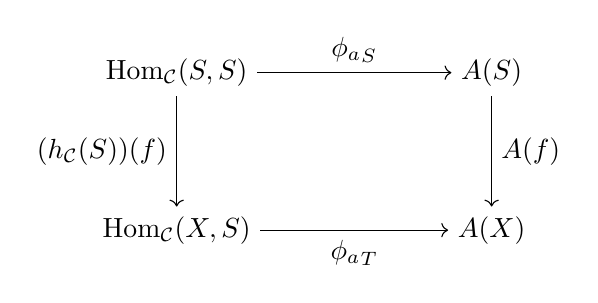
\begin{tikzpicture}
                \node (HSS) at (-2,1) {\(\mathrm{Hom}_{\mathcal{C}} (S,S)\)};
                \node (HXS) at (-2,-1) {\(\mathrm{Hom}_{\mathcal{C}} (X,S)\)};
                \node (AS) at (2,1) {\(A(S)\)};
                \node (AX) at (2,-1) {\(A(X)\)};
                \draw[->] (HSS) to node[left] {\((h_{\mathcal{C}} (S)) (f)\)} (HXS);
                \draw[->] (AS) to node[right] {\(A(f)\)} (AX);
                \draw[->] (HSS) to node[above] {\({\phi_a}_S\)} (AS);
                \draw[->] (HXS) to node[below] {\({\phi_a}_T\)} (AX);
            \end{tikzpicture}
        \end{center}

        自然性展开符号即可, 同构基于 \ref{lemma:natural transformation is isomorphism iff each component is isomorphism}.
    \end{proof}
\end{lemma}

\begin{lemma}
    上述 \(h_\mathcal{C}\) 是全忠实函子, 给出了自然的嵌入 \(\mathcal{C} \to \mathcal{C}^{\wedge}\).

    \begin{proof}
        全忠实性考虑取 \(A\) 为 \(h_\mathcal{C}(T)\), \ref{lemma:Yoneda lemma} 即给出 \(\mathrm{Hom}_{\mathcal{C}^{\wedge}} (h_{\mathcal{C}} (S), h_{\mathcal{C}} (T))\), \(\mathrm{Hom}_{\mathcal{C}} (S,T)\)
        间双射.
    \end{proof}
\end{lemma}

\begin{corollary}
    对称的, \(k_\mathcal{C}\) 全忠实, 且有自然的函子同构 \(\mathrm{Hom}_{\mathcal{C}^{\vee}} (k_{\mathcal{C}} (-), -) \to \mathrm{ev}^{\vee}\).

    \begin{proof}
        只需注意到恒等式 \({(\mathcal{C}^{\vee})}^\mathrm{op} = {(\mathcal{C}^{\mathrm{op}})}^{\wedge}\).
    \end{proof}
\end{corollary}

\begin{definition}[可表]
    称预层 \(A\) 可表 (representable) 当且仅当存在对象 \(S \in \mathcal{C}\) 并给出 \(A \cong h_{\mathcal{C}} (S)\) 的同构 \(\phi : h_{\mathcal{C}} (S) \to A\),
    并称 \((S,\phi)\) 是 \(A\) 的代表元, 对 \(B \in \mathbf{Fun} (\mathcal{C},\mathbf{Set})\) 亦然.
\end{definition}

\begin{lemma}
    代表元若存在则在同构意义下唯一.

    \begin{proof}
        利用米田嵌入的全忠实性.
    \end{proof}
\end{lemma}

\subsection{伴随对}

\begin{definition}[伴随]
    给出函子 \(F : \mathcal{C} \to \mathcal{D}\), \(G : \mathcal{D} \to \mathcal{C}\), 
    与自然变换 \(\eta : \mathrm{id}_{\mathcal{C}} \to G \circ F\), \(\varepsilon : F \circ G \to \mathrm{id}_{\mathcal{D}}\),
    使得以下两图表合成为恒等自然变换:

    \begin{center}
        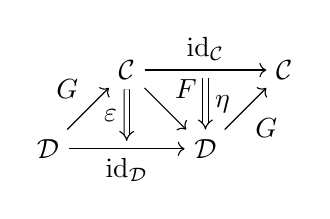
\begin{tikzpicture}
            \node (C1) at (-0.5,0.5) {\(\mathcal{C}\)};
            \node (C2) at (1.5,0.5) {\(\mathcal{C}\)};
            \node (D1) at (-1.5,-0.5) {\(\mathcal{D}\)};
            \node (D2) at (0.5,-0.5) {\(\mathcal{D}\)};
            \draw[->] (C1) to node[above] (idc) {\(\mathrm{id}_{\mathcal{C}}\)} (C2);
            \draw[->] (D1) to node[below] (idd) {\(\mathrm{id}_{\mathcal{D}}\)} (D2);
            \draw[->] (D1) to node[above left] {\(G\)} (C1);
            \draw[->] (D2) to node[below right] {\(G\)} (C2);
            \draw[->] (C1) to node[above right] {\(F\)} (D2);
            \draw[-{Implies},double,double distance = 0.15em] (C1) to node[left] {\(\varepsilon\)} ($(idd.north) + (0,0.1)$);
            \draw[-{Implies},double,double distance = 0.15em] ($(idc.south) + (0,-0.1)$) to node[right] {\(\eta\)} (D2);
        \end{tikzpicture} 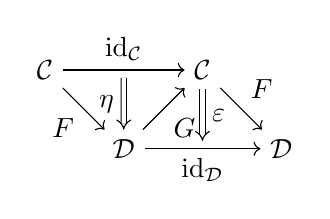
\begin{tikzpicture}
            \node (C1) at (-1.5,0.5) {\(\mathcal{C}\)};
            \node (C2) at (0.5,0.5) {\(\mathcal{C}\)};
            \node (D1) at (-0.5,-0.5) {\(\mathcal{D}\)};
            \node (D2) at (1.5,-0.5) {\(\mathcal{D}\)};
            \draw[->] (C1) to node[above] (idc) {\(\mathrm{id}_{\mathcal{C}}\)} (C2);
            \draw[->] (D1) to node[below] (idd) {\(\mathrm{id}_{\mathcal{D}}\)} (D2);
            \draw[->] (C1) to node[below left] {\(F\)} (D1);
            \draw[->] (C2) to node[above right] {\(F\)} (D2);
            \draw[->] (D1) to node[below right] {\(G\)} (C2);
            \draw[-{Implies},double,double distance = 0.15em] (C2) to node[right] {\(\varepsilon\)} ($(idd.north) + (0,0.1)$);
            \draw[-{Implies},double,double distance = 0.15em] ($(idc.south) + (0,-0.1)$) to node[left] {\(\eta\)} (D1);
        \end{tikzpicture}
    \end{center}

    写成合成为:

    \[
        (\mathrm{id}_{G} \ast \varepsilon) \circ (\eta \ast \mathrm{id}_{G}) = \mathrm{id}_{G}, (\varepsilon \ast \mathrm{id}_{F}) \circ (\mathrm{id}_{F} \ast \eta) = \mathrm{id}_{F}
    \]

    称 \(F\) 为 \(G\) 的左伴随 (left adjoint), \(G\) 为 \(F\) 的右伴随 (right adjoint), 记为 \(F \dashv G\).
\end{definition}

\begin{lemma}
    \(F\) 是 \(G\) 左伴随当且仅当有 \(\mathcal{C}^{\mathrm{op}} \times \mathcal{D} \to \mathbf{Set}\) 中函子
    \(\mathrm{Hom}_{\mathcal{D}} (F (-), -)\) 与 \(\mathrm{Hom}_{\mathcal{C}} (-, G (-))\) 同构.

    \begin{proof}
        我们的任务是找到这样一个一一对应, 这里的技术在于把映射变成拉回推出.

        假定我们给出伴随函子 \(F,G\) 和 \(f \in \mathrm{Hom}_{\mathcal{D}} (F (X), Y)\), 构造
        \(\varphi(f) : X \to G (Y)\) 为 \(G (f) \circ \eta_X\); 对 \(g \in \mathrm{Hom}_{\mathcal{C}} (X, G(Y))\) 构造
        \(\varphi^{-1} (g) : F(X) \to Y\) 为 \(\varepsilon_Y \circ F (g)\).

        而 \(\varphi^{-1} \varphi (f) = \varepsilon_{Y} \circ F (G (f) \circ \eta_X) = (\varepsilon_Y \circ FG f) \circ \eta_X = f \circ \varepsilon_{F(X)} \circ F (\eta_X) = f\),
        \(\varphi \varphi^{-1} (g) = G(\varepsilon_Y \circ F(g)) \circ \eta_X = G (\varepsilon_Y) \circ (GF (g) \circ \eta_{X}) = G (\varepsilon_Y) \circ \eta_{G(Y)} \circ g = g\).

        接下来验证 \(\varphi\) 自然性, \(\varphi(a \circ f \circ F(b)) = G(a) \circ G(f) \circ GF (b) \circ \eta_{X^\prime} = G(a) \circ G(f) \circ \eta_X \circ b\),
        \(\varphi^{-1} (G(a) \circ g \circ b) = \varepsilon_{Y^\prime} \circ FG(a) \circ F(g) \circ F(b) = a \circ \varepsilon_Y \circ F(g) \circ F(b)\).

        反之, 给出 \(\varphi\) 与 \(\varphi^{-1}\), 定义 \(\eta_X := \varphi (\mathrm{id}_{F(X)})\), \(\varepsilon_Y := \varphi^{-1} (\mathrm{id}_{G(Y)})\),
        自然性继承自 \(\varphi\) 与 \(\varphi^{-1}\) 的自然性.

        需验证上述自然变换合成等式 \(G \varepsilon_Y \circ \eta_{G(Y)} = \varphi \varphi^{-1} (\mathrm{id}_{G(Y)} \circ \mathrm{id}_{FGY}) = \mathrm{id}_{G(Y)}\),
        \(\varepsilon_{F(X)} \circ F \eta_X = \varphi^{-1} \varphi (\mathrm{id}_{F(X)} \circ \mathrm{id}_{F \eta_X}) = \mathrm{id}_{F(X)}\).
    \end{proof}
\end{lemma}

上述引理给出了伴随对在 \(\mathrm{Hom}\) 集上的体现, 于是我们可以考虑伴随与可表的关系.

\begin{lemma}
    函子 \(F : \mathcal{C} \to \mathcal{D}\) 有右伴随当且仅当 \(\mathrm{Hom}_{\mathcal{D}} (F (-), Y)\) 对每个 \(Y\) 皆可表.

    \begin{proof}
        我们利用可表函子显式的逐点表示出 \(G\).

        对任意 \(Y\), 假定上述函子被 \((S_Y, \phi_Y)\) 表, 则构造出函子 \(G\) 使得 \(G(Y) = S_Y\),
        对于映射 \(f : Y \to Y^\prime\), 令 \(G(f) : S_Y \to S_{Y^\prime}\) 为与 \({\phi_{Y^\prime}}^{-1} \circ h_{\mathcal{C}} (f) \circ \phi_Y \in \mathrm{Mor} (\mathcal{C}^{\wedge})\)
        对应的唯一映射, 则函子性自然归结于 \(h_\mathcal{C}\) 的函子性.

        注意到 \({(\phi_Y)}_X\) 自然给出了 \(\mathrm{Hom}_{\mathcal{D}} (F (X), Y) \to \mathrm{Hom}_{\mathcal{C}} (X, G(Y))\),
        而用 \(\phi\) 在 \(X\) 处自然性源于 \(\phi_Y\) 的自然性, 在 \(Y\) 处自然性源于 \(G(f)\) 定义确保了在 \(\mathcal{C}^{\wedge}\) 中的自然性, 亦 \(\mathcal{C}\) 中的自然性.
    \end{proof}
\end{lemma}

\begin{corollary}
    同理, \(G\) 有左伴随当且仅当 \(\mathrm{Hom}_{\mathcal{C}} (X, G (-))\) 对每个 \(X\) 皆可表.
\end{corollary}

\begin{lemma}
    一个函子的左伴随若存在则在同构意义下唯一, 右伴随亦然.

    \begin{proof}
        运用上题的想法, 既已给出了 \(\mathcal{C}^{\wedge}\) 中的同构, 则亦是 \(\mathcal{C}\) 中的同构,
        该同构自然性亦通过 \(\mathcal{C}^{\wedge}\) 中保存.
    \end{proof}
\end{lemma}

\begin{lemma}
    给出范畴 \(\mathcal{C}_1, \mathcal{C}_2, \mathcal{C}_3\), 与函子 \(F : \mathcal{C}_1 \to \mathcal{C}_2\), \(G : \mathcal{C}_2 \to \mathcal{C}_1\),
    \(F^\prime : \mathcal{C}_2 \to \mathcal{C}_3\), \(G^\prime : \mathcal{C}_3 \to \mathcal{C}_2\), 使得 \(F \dashv G\), \(F^\prime \dashv G^\prime\),
    则 \(F^\prime \circ F \dashv G \circ G^\prime\).

    \begin{center}
        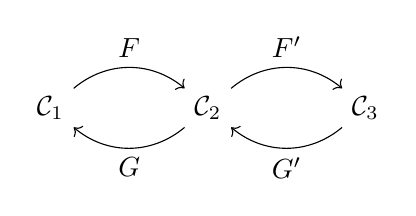
\begin{tikzpicture}
            \node (C1) at (-2,0) {\(\mathcal{C}_1\)};
            \node (C2) at (0,0) {\(\mathcal{C}_2\)};
            \node (C3) at (2,0) {\(\mathcal{C}_3\)};
            \draw[->] (C1) to [bend left = 40] node[above] {\(F\)} (C2);
            \draw[->] (C2) to [bend left = 40] node[above] {\(F^\prime\)} (C3);
            \draw[->] (C2) to [bend left = 40] node[below] {\(G\)} (C1);
            \draw[->] (C3) to [bend left = 40] node[below] {\(G^\prime\)} (C2);
        \end{tikzpicture}
    \end{center}

    \begin{proof}
        给出伴随对应的自然变换 \(\eta, \eta^\prime, \varepsilon, \varepsilon^\prime\),
        定义 \(\xi := (\mathrm{id}_G \ast \eta^\prime \mathrm{id}_{F}) \circ \eta\),
        \(\zeta := \varepsilon^\prime \ast (\varepsilon \ast \mathrm{id}_{G^\prime}) \circ \mathrm{id}_F\),

        \(\xi, \zeta\) 给出 \(F^\prime \circ F \dashv G \circ G^\prime\), 观察以下图表:

        \begin{center}
            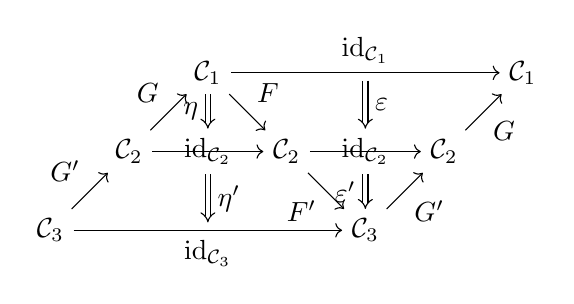
\begin{tikzpicture}
                \node (C11) at (-1,1) {\(\mathcal{C}_1\)};
                \node (C12) at (3,1) {\(\mathcal{C}_1\)};
                \node (C21) at (-2,0) {\(\mathcal{C}_2\)};
                \node (C22) at (0,0) {\(\mathcal{C}_2\)};
                \node (C23) at (2,0) {\(\mathcal{C}_2\)};
                \node (C31) at (-3,-1) {\(\mathcal{C}_3\)};
                \node (C32) at (1,-1) {\(\mathcal{C}_3\)};
                \draw[->] (C11) to node[above] (idc1) {\(\mathrm{id}_{\mathcal{C}_1}\)} (C12);
                \draw[->] (C21) to node (idc21) {\(\mathrm{id}_{\mathcal{C}_2}\)} (C22);
                \draw[->] (C22) to node (idc22) {\(\mathrm{id}_{\mathcal{C}_2}\)} (C23);
                \draw[->] (C31) to node[below] (idc3) {\(\mathrm{id}_{\mathcal{C}_3}\)} (C32);
                \draw[->] (C31) to node[above left] {\(G^\prime\)} (C21);
                \draw[->] (C21) to node[above left] {\(G\)} (C11);
                \draw[->] (C11) to node[above right] {\(F\)} (C22);
                \draw[->] (C22) to node[below left] {\(F^\prime\)} (C32);
                \draw[->] (C32) to node[below right] {\(G^\prime\)} (C23);
                \draw[->] (C23) to node[below right] {\(G\)} (C12);
                \draw[-{Implies},double,double distance = 0.15em] (C11) to node[left] {\(\eta\)} (idc21);
                \draw[-{Implies},double,double distance = 0.15em] (idc21) to node[right] {\(\eta^\prime\)} ($(idc3.north) + (0,0.1)$);
                \draw[-{Implies},double,double distance = 0.15em] (idc22) to node[left] {\(\varepsilon^\prime\)} (C32);
                \draw[-{Implies},double,double distance = 0.15em] ($(idc1.south) + (0,-0.1)$) to node[right] {\(\varepsilon\)} (idc22);
            \end{tikzpicture}
        \end{center}

        此图表合成 \(\mathrm{id}_{G \circ G^\prime}\) 只需注意到上下两个平行四边形均合成单位自然变换, 而左右两个大三角形分别代表 \(\xi, \zeta\),
        另一个图表同理合成 \(\mathrm{id}_{F^\prime \circ F}\).
    \end{proof}
\end{lemma}

\begin{definition}
    我们定义 \(2\) - 范畴为满足如下条件的范畴:

    \begin{enumerate}
        \item 一个范畴 \(\mathcal{C}\).
        \item 任取 \(X,Y \in \mathrm{Ob} (\mathcal{C})\), 有范畴 \(\mathcal{D}\) 使得 \(\mathrm{Mor} (\mathcal{D}) = \mathrm{Hom}_\mathcal{C} (X,Y)\).
        \item 有横合成, 给出 \(f, f^\prime \in \mathrm{Hom}_\mathcal{C} (X,Y)\), \(g, g^\prime \in \mathrm{Hom}_\mathcal{C} (Y,Z)\), 与
                \(2\) - 态射 \(\phi : f \to f^\prime\), \(\psi : g \to g^\prime\), 存在态射 \(\phi \ast \psi : g \circ f \to g^\prime \circ f^\prime\).
        \item 横合成结合, 且与纵合成交换.
        \item 两个单位横合成仍是单位.
    \end{enumerate}
\end{definition}

记原范畴的元素为 \(\mathrm{Mor}_0\), 原范畴的态射为 \(\mathrm{Mor}_1\), 称 \(1\) - 态射, \(2\) - 态射记为 \(\mathrm{Mor}_2\).

\begin{example}
    \(\mathbf{Cat}\) 是 \(2\) - 范畴, 对象是全体范畴, 态射是范畴间的函子, \(2\) - 态射是自然变换.
\end{example}

我们可以绘制 \(2\) - 范畴对应的图表, 用 \(\Rightarrow\) 表示 \(2\) - 态射, 依旧用 \(\mathrm{Hom}\) 表示两点间态射对应的范畴.

\begin{definition}[Kan 延拓]
    在 \(2\) - 范畴 \(\Theta\) 中给出对象 \(\mathcal{C},\mathcal{D},\mathcal{E} \in \mathrm{Mor}_0 (\Theta)\),
    给出 \(1\) - 态射 \(F : \mathcal{C} \to \mathcal{E}, K : \mathcal{C} \to \mathcal{D}\).

    定义左 Kan 延拓 \(\mathrm{Lan}_K F : \mathcal{D} \to \mathcal{E}\) 与其对应的 \(2\) - 态射 \(\eta : F \to \mathrm{Lan}_K F \circ K\),
    满足任给 \(G : \mathcal{D} \to \mathcal{E}\) 与 \(2\) - 态射 \(\phi : F \to G \circ K\), 存在唯一的 \(2\) - 态射 \(\phi^\prime : \mathrm{Lan}_K F \to G\), 满足以下等式:

    \[
        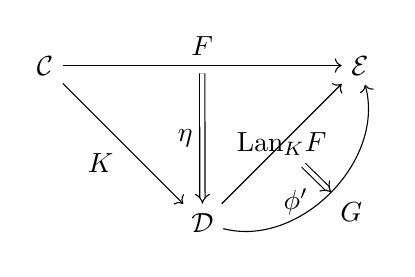
\begin{tikzpicture}
            \node (C) at (-2,2) {\(\mathcal{C}\)};
            \node (D) at (0,0) {\(\mathcal{D}\)};
            \node (E) at (2,2) {\(\mathcal{E}\)};
            \draw[->] (C) to node[above] (F) {\(F\)} (E);
            \draw[->] (C) to node[below left] {\(K\)} (D);
            \draw[->] (D) to [bend right = 60] node[below right] (G) {\(G\)} (E);
            \draw[->] (D) to node (Lan) {\(\mathrm{Lan}_K F\)} (E);
            \draw[-{Implies},double,double distance = 0.15em] ($(F.south) + (0 , - 0.1)$) to node[left] {\(\eta\)} (D);
            \draw[-{Implies},double,double distance = 0.15em] (Lan) to node[below left] {\(\phi^\prime\)} (G);
        \end{tikzpicture} = 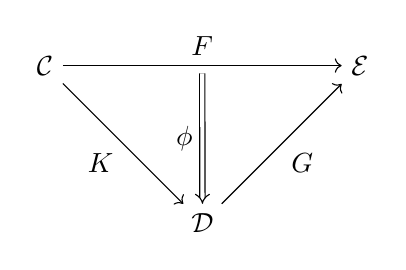
\begin{tikzpicture}
            \node (C) at (-2,2) {\(\mathcal{C}\)};
            \node (D) at (0,0) {\(\mathcal{D}\)};
            \node (E) at (2,2) {\(\mathcal{E}\)};
            \draw[->] (C) to node[above] (F) {\(F\)} (E);
            \draw[->] (C) to node[below left] {\(K\)} (D);
            \draw[->] (D) to node[below right] (G) {\(G\)} (E);
            \draw[-{Implies},double,double distance = 0.15em] ($(F.south) + (0 , - 0.1)$) to node[left] {\(\phi\)} (D);
        \end{tikzpicture}
    \]

    对偶的, 定义右 Kan 延拓 \(\mathrm{Ran}_K F : \mathcal{D} \to \mathcal{E}\) 与其对应的 \(2\) - 态射 \(\varepsilon : \mathrm{Ran}_K F \circ K \to F\),
    满足任给 \(G : \mathcal{D} \to \mathcal{E}\) 与 \(2\) - 态射 \(\phi : G \circ K \to F\), 存在唯一的 \(2\) - 态射 \(\phi^\prime : G \to \mathrm{Ran}_K F\), 满足以下等式:

    \[
        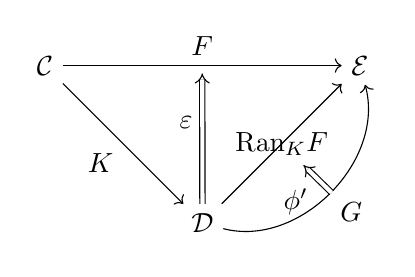
\begin{tikzpicture}
            \node (C) at (-2,2) {\(\mathcal{C}\)};
            \node (D) at (0,0) {\(\mathcal{D}\)};
            \node (E) at (2,2) {\(\mathcal{E}\)};
            \draw[->] (C) to node[above] (F) {\(F\)} (E);
            \draw[->] (C) to node[below left] {\(K\)} (D);
            \draw[->] (D) to [bend right = 60] node[below right] (G) {\(G\)} (E);
            \draw[->] (D) to node (Ran) {\(\mathrm{Ran}_K F\)} (E);
            \draw[-{Implies},double,double distance = 0.15em] (D) to node[above left] {\(\varepsilon\)} ($(F.south) + (0 , - 0.1)$);
            \draw[-{Implies},double,double distance = 0.15em] (G) to node[below left] {\(\phi^\prime\)} (Ran);
        \end{tikzpicture} = 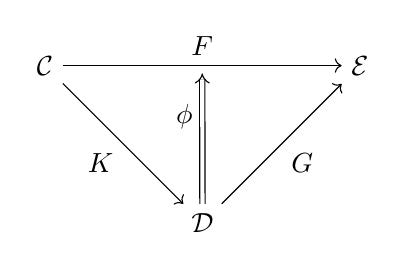
\begin{tikzpicture}
            \node (C) at (-2,2) {\(\mathcal{C}\)};
            \node (D) at (0,0) {\(\mathcal{D}\)};
            \node (E) at (2,2) {\(\mathcal{E}\)};
            \draw[->] (C) to node[above] (F) {\(F\)} (E);
            \draw[->] (C) to node[below left] {\(K\)} (D);
            \draw[->] (D) to node[below right] (G) {\(G\)} (E);
            \draw[-{Implies},double,double distance = 0.15em] (D) to node[above left] {\(\phi\)} ($(F.south) + (0 , - 0.1)$);
        \end{tikzpicture}
    \]
\end{definition}

\begin{lemma}
    Kan 延拓存在则在同构意义下唯一.

    \begin{proof}
        利用泛性质唯一性.
    \end{proof}
\end{lemma}

\begin{lemma}
    如若所有 \(F : \mathcal{C} \to \mathcal{E}\) 的右 Kan 延拓存在, 则 \(\mathrm{Ran}_K\) 给出
    从 \(\mathrm{Hom} (\mathcal{C}, \mathcal{E})\) 到 \(\mathrm{Hom} (\mathcal{D}, \mathcal{E})\) 的函子.

    \begin{proof}
        需给出 \(\mathrm{Ran}_K\) 对态射的作用, 给出 \(F \to G\) 的态射 \(\phi : F \to G\), 定义 \(\mathrm{Ran}_K \phi\) 为使得以下等式成立的唯一态射:

        \[
            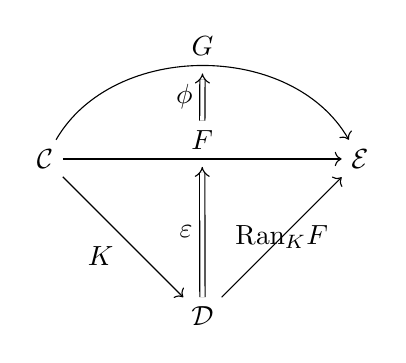
\begin{tikzpicture}
                \node (C) at (-2,2) {\(\mathcal{C}\)};
                \node (D) at (0,0) {\(\mathcal{D}\)};
                \node (E) at (2,2) {\(\mathcal{E}\)};
                \draw[->] (C) to node[above] (F) {\(F\)} (E);
                \draw[->] (C) to [bend left = 60] node[above] (G) {\(G\)} (E);
                \draw[->] (C) to node[below left] {\(K\)} (D);
                \draw[->] (D) to node (Ran) {\(\mathrm{Ran}_K F\)} (E);
                \draw[-{Implies},double,double distance = 0.15em] (D) to node[left] {\(\varepsilon\)} ($(F.south) + (0 , - 0.1)$);
                \draw[-{Implies},double,double distance = 0.15em] (F) to node[left] {\(\phi\)} ($(G.south) + (0 , - 0.1)$);
            \end{tikzpicture} = 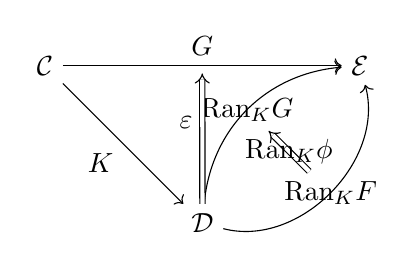
\begin{tikzpicture}
                \node (C) at (-2,2) {\(\mathcal{C}\)};
                \node (D) at (0,0) {\(\mathcal{D}\)};
                \node (E) at (2,2) {\(\mathcal{E}\)};
                \draw[->] (C) to node[above] (G) {\(G\)} (E);
                \draw[->] (C) to node[below left] {\(K\)} (D);
                \draw[->] (D) to [bend left = 40] node (RanG) {\(\mathrm{Ran}_K G\)} (E);
                \draw[->] (D) to [bend right = 60] node (RanF) {\(\mathrm{Ran}_K F\)} (E);
                \draw[-{Implies},double,double distance = 0.15em] (RanF) to node {\(\mathrm{Ran}_K \phi\)} (RanG);
                \draw[-{Implies},double,double distance = 0.15em] (D) to node[above left] {\(\varepsilon\)} ($(G.south) + (0 , - 0.1)$);
            \end{tikzpicture}
        \]

        函子性由唯一性保证.
    \end{proof}
\end{lemma}

\begin{corollary}
    同理, 假定对于所有 \(F : \mathcal{C} \to \mathcal{E}\) 的左 Kan 延拓存在, 则 \(\mathrm{Lan}_K\) 也给出
    从 \(\mathrm{Hom} (\mathcal{C}, \mathcal{E})\) 到 \(\mathrm{Hom} (\mathcal{D}, \mathcal{E})\) 的函子.
\end{corollary}

\begin{lemma}
    有伴随对 \(\mathrm{Lan}_K \dashv (- \circ K) \dashv \mathrm{Ran}_K\), 其中 \((- \circ K)\) 
    定义为将 \(1\) - 态射合成 \(K\), 而将 \(2\) - 态射横合成 \(\mathrm{id}_K\).

    \begin{proof}
        态射集 \(\mathrm{Hom}_{\mathrm{Hom} (\mathcal{D}, \mathcal{E})} (\mathrm{Lan}_K (F),G) \to \mathrm{Hom}_{\mathrm{Hom} (\mathcal{C}, \mathcal{E})} (F,G \circ K)\)
        无非是定义的复写. 在 \(F\) 处自然性是按 \(\mathrm{Lan}_K\) 对态射变换的定义, 在  \(G\) 处的自然性依赖唯一性.
    \end{proof}
\end{lemma}

\begin{lemma}
    在 \(\mathbf{Cat}\) 中考虑, 伴随对 \(F \dashv G\) 给出 Kan 延拓 \(G = \mathrm{Lan}_F (\mathrm{id}_\mathcal{C})\), \(F = \mathrm{Ran}_G (\mathrm{id}_\mathcal{C})\).

    \begin{proof}
        观察下图的合成

        \begin{center}
            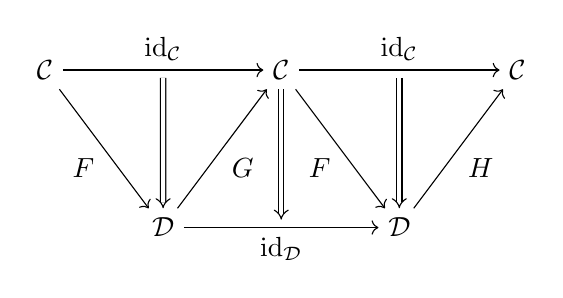
\begin{tikzpicture}
                \node (C1) at (-3,1) {\(\mathcal{C}\)};
                \node (C2) at (0,1) {\(\mathcal{C}\)};
                \node (C3) at (3,1) {\(\mathcal{C}\)};
                \node (D1) at (-1.5,-1) {\(\mathcal{D}\)};
                \node (D2) at (1.5,-1) {\(\mathcal{D}\)};
                \draw[->] (C1) to node[above] (idc1) {\(\mathrm{id}_{\mathcal{C}}\)} (C2);
                \draw[->] (C2) to node[above] (idc2) {\(\mathrm{id}_{\mathcal{C}}\)} (C3);
                \draw[->] (D1) to node[below] (idd) {\(\mathrm{id}_{\mathcal{D}}\)} (D2);
                \draw[->] (C1) to node[below left] {\(F\)} (D1);
                \draw[->] (C2) to node[below left] {\(F\)} (D2);
                \draw[->] (D1) to node[below right] {\(G\)} (C2);
                \draw[->] (D2) to node[below right] {\(H\)} (C3);
                \draw[-{Implies},double,double distance = 0.15em] ($(idc1.south) + (0,-0.1)$) to (D1);
                \draw[-{Implies},double,double distance = 0.15em] (C2) to ($(idd.north) + (0,0.1)$);
                \draw[-{Implies},double,double distance = 0.15em] ($(idc2.south) + (0,-0.1)$) to (D2);
            \end{tikzpicture}
        \end{center}

        所需 \(2\) 态射为右侧平行四边形, 另一个方向亦然.
    \end{proof}
\end{lemma}

\subsection{极限}

定义 \(\mathbf{1}\) 为最简单的范畴, 仅有一个对象与一个态射, 记为 \(\bullet\), 任何
范畴都有唯一的函子 \(\mathbf{1} \to \mathcal{C}\).

\begin{definition}[极限]
    在范畴 \(\mathbf{Cat}\) 中考虑.
    
    给出小范畴 \(I\) 与函子 \(F : I \to \mathcal{C}\), \(K : I \to \mathbf{1}\), 
    若 \(\mathrm{Ran}_K F\) 存在, 则称 \(\mathrm{Ran}_K F\) 为 \(F\) 的极限 (limit), 记为 \(\varprojlim F\),
    对称的 \(\mathrm{Lan}_K F\) 称为 \(F\) 的余极限 (colimit), 记为 \(\varinjlim F\), 称 \(I^\mathrm{op}\) 为极限对应的指标, \(I\) 为余极限对应的指标.
\end{definition}

解释一下上述对于极限的定义, 给出一个 \(\mathbf{1}\) 出发的函子, 即选中了 \(\mathcal{C}\) 中的一个对象 (此对象沿用上述符号记作 \(\varprojlim F\) 或 \(\varinjlim F\)),
极限构造中上述 Kan 延拓给出的自然变换标记了从该对象出发的函子到 \(F I\) 中一对象的态射, 满足对于任意 \(f \in \mathrm{Mor}(I)\), 下图交换:

\begin{center}
    \begin{tikzpicture}
        \node (FX) at (-2,2) {\(F X\)};
        \node (FY) at (2,2) {\(F Y\)};
        \node (lim) at (0,0) {\(\varprojlim F\)};
        \draw[->] (FX) to node[above] (Ff) {\(F f\)} (FY);
        \draw[->] (lim) to (FX);
        \draw[->] (lim) to (FY);
    \end{tikzpicture}
\end{center}

Kan 延拓的性质也就被解为, 对于任意给出的 \(L \in \mathcal{C}\), 一族态射 \(\phi_X : L \to F X\), 使得对于任意 \(f \in \mathrm{Mor}(I)\), 下图交换:

\begin{center}
    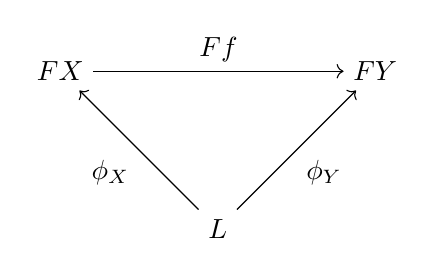
\begin{tikzpicture}
        \node (FX) at (-2,2) {\(F X\)};
        \node (FY) at (2,2) {\(F Y\)};
        \node (L) at (0,0) {\(L\)};
        \draw[->] (FX) to node[above] (Ff) {\(F f\)} (FY);
        \draw[->] (L) to node[below left] (phiX) {\(\phi_X\)} (FX);
        \draw[->] (L) to node[below right] (phiY) {\(\phi_Y\)} (FY);
    \end{tikzpicture}
\end{center}

都有唯一的态射 \(\phi_f : L \to \varprojlim F\), 使得对于任意 \(X \in \mathrm{Ob} (I)\) 下图交换:

\begin{center}
    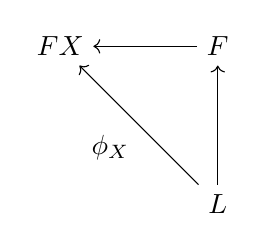
\begin{tikzpicture}
        \node (FX) at (-2,2) {\(F X\)};
        \node (L) at (0,0) {\(L\)};
        \node (lim) at (0,2) {\(\varprojlim F\)};
        \draw[->] (lim) to (FX);
        \draw[->] (L) to node[below left] (phiX) {\(\phi_X\)} (FX);
        \draw[->] (L) to (lim);
    \end{tikzpicture}
\end{center}

余极限将上述所有箭头反向即可得到.

\begin{definition}
    直积 (product) 与余积 (coproduct) 是极限与余极限的特例, 分别对应于 \(I\) 为离散范畴的极限与余极限.
\end{definition}

\begin{example}
    \(\mathbf{Set}\) 中直积为笛卡尔积, 余积为不交并.
\end{example}

\begin{definition}
    等化子 (equalizer) 与余等化子 (coequalizer) 是极限与余极限的特例, 分别对应于 \(I\) 为下图所示的范畴的极限与余极限 (\(\mathrm{id}\) 未画出).

    \begin{center}
        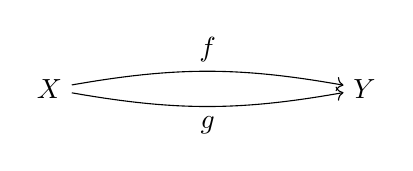
\begin{tikzpicture}
            \node (X) at (-2,0) {\(X\)};
            \node (Y) at (2,0) {\(Y\)};
            \draw[->] (X) to [bend left = 10] node[above] (f) {\(f\)} (Y);
            \draw[->] (X) to [bend right = 10] node[below] (g) {\(g\)} (Y);
        \end{tikzpicture}
    \end{center}
\end{definition}

\begin{lemma}
    \label {lemma:existence of limitation of homeomorphism}
    给出自然变换 \(\psi : \alpha \to \alpha^\prime\), 假使极限存在则存在唯一 \(\psi\) 使对任意 \(i\) 以下图表交换:

    \begin{center}
        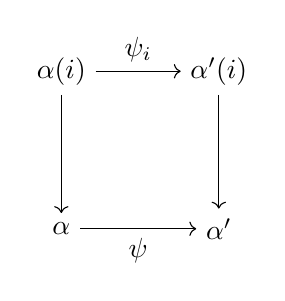
\begin{tikzpicture}
            \node (ai) at (-1,1) {\(\alpha (i)\)};
            \node (api) at (1,1) {\(\alpha^\prime (i)\)};
            \node (lima) at (-1,-1) {\(\varinjlim \alpha\)};
            \node (limap) at (1,-1) {\(\varinjlim \alpha^\prime\)};
            \draw[->] (ai) to node[above] (aii) {\(\psi_i\)} (api);
            \draw[->] (ai) to (lima);
            \draw[->] (api) to (limap);
            \draw[->] (lima) to node[below] (limf) {\(\varinjlim \psi\)} (limap);
        \end{tikzpicture}
    \end{center}

    \begin{proof}
        态射合成给出了 \(\alpha(i) \to \varinjlim \alpha^\prime\), 其与 \(\mathrm{Mor}(I)\) 相容, 由极限的定义唯一性给出了 \(\varinjlim \alpha \to \varinjlim \alpha^\prime\).
    \end{proof}
\end{lemma}

\begin{corollary}
    给出自然变换 \(\psi : \alpha \to \alpha^\prime\), 假使极限存在则存在唯一 \(\psi\) 使对任意 \(i\) 以下图表交换:

    \begin{center}
        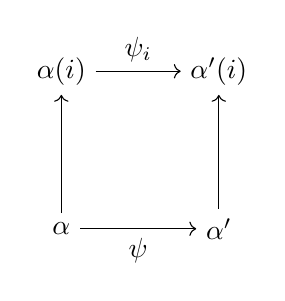
\begin{tikzpicture}
            \node (ai) at (-1,1) {\(\alpha (i)\)};
            \node (api) at (1,1) {\(\alpha^\prime (i)\)};
            \node (lima) at (-1,-1) {\(\varprojlim \alpha\)};
            \node (limap) at (1,-1) {\(\varprojlim \alpha^\prime\)};
            \draw[->] (ai) to node[above] (aii) {\(\psi_i\)} (api);
            \draw[->] (lima) to (ai);
            \draw[->] (limap) to (api);
            \draw[->] (lima) to node[below] (limf) {\(\varprojlim \psi\)} (limap);
        \end{tikzpicture}
    \end{center}
\end{corollary}

\begin{lemma}
    给出自然变换 \(\psi : \alpha_1 \to \alpha_2\),  \(\phi : \alpha_2 \to \alpha_3\), 假使极限存在则有等式 \(\varinjlim (\phi \psi) = \varinjlim \phi \varinjlim \psi\).

    \begin{proof}
            无非是交换图表:

            \begin{center}
                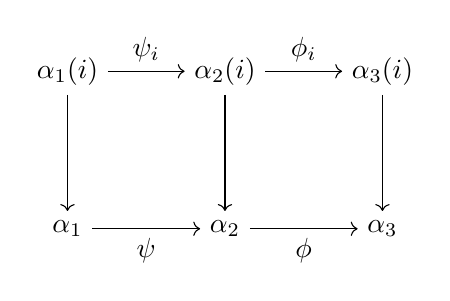
\begin{tikzpicture}
                    \node (a1i) at (-2,1) {\(\alpha_1 (i)\)};
                    \node (a2i) at (0,1) {\(\alpha_2 (i)\)};
                    \node (a3i) at (2,1) {\(\alpha_3 (i)\)};
                    \node (lima1) at (-2,-1) {\(\varinjlim \alpha_1\)};
                    \node (lima2) at (0,-1) {\(\varinjlim \alpha_2\)};
                    \node (lima3) at (2,-1) {\(\varinjlim \alpha_3\)};
                    \draw[->] (a1i) to node[above] (psi) {\(\psi_i\)} (a2i);
                    \draw[->] (a2i) to node[above] (phi) {\(\phi_i\)} (a3i);
                    \draw[->] (a1i) to (lima1);
                    \draw[->] (a2i) to (lima2);
                    \draw[->] (a3i) to (lima3);
                    \draw[->] (lima1) to node[below] (limpsi) {\(\varinjlim \psi\)} (lima2);
                    \draw[->] (lima2) to node[below] (limphi) {\(\varinjlim \phi\)} (lima3);
                \end{tikzpicture}
            \end{center}
    \end{proof}
\end{lemma}

\begin{corollary}
    同理有等式 \(\varprojlim (\phi \psi) = \varprojlim \phi \varprojlim \psi\).
\end{corollary}

\begin{lemma}
    直积的直积 (余积的余积) 为直积 (余积).

    \begin{proof}
        给出对象 \(X_{i,j}\) 的直积 \(X_{i} := \prod_j X_{i,j}\) 与直积 \(X := \prod_i X_i\),
        无非是说对于任意对象 \(Y\), \(\prod_{i,j} \mathrm{Hom} (Y,X_{i,j})\) 与 \(\prod_i \mathrm{Hom} (Y,X_i)\), \(\mathrm{Hom} (Y,X)\) 一一对应,
        老直积态射的合成给出新直积所需的态射.
    \end{proof}
\end{lemma}

\begin{definition}
    考察以下范畴 \(I\):

    \begin{center}
        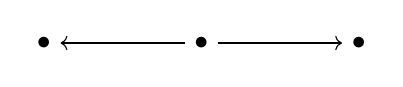
\begin{tikzpicture}
            \node (B1) at (-2,0) {\(\bullet\)};
            \node (B2) at (0,0) {\(\bullet\)};
            \node (B3) at (2,0) {\(\bullet\)};
            \draw[->] (B2) to (B1);
            \draw[->] (B2) to (B3);
        \end{tikzpicture}
    \end{center}

    以 \(I\) 为指标的极限称纤维积 (fibre product) 或拉回 (pullback), \(I\) 的余极限称纤维余积或推出 (pushout), 记作 Cartesius 图表:

    \begin{center}
        \begin{tikzpicture}
            \node (prod) at (-1,1) {\(X \times_Z Y\)};
            \node (X) at (1,1) {\(X\)};
            \node (Y) at (-1,-1) {\(Y\)};
            \node (Z) at (1,-1) {\(Z\)};
            \draw[->] (X) to (Z);
            \draw[->] (Y) to (Z);
            \draw[->] (prod) to (X);
            \draw[->] (prod) to (Y);
            \node at (0,0) {\(\Box\)};
        \end{tikzpicture} \begin{tikzpicture}
            \node (coprod) at (-1,1) {\(X \sqcup_Z Y\)};
            \node (X) at (1,1) {\(X\)};
            \node (Y) at (-1,-1) {\(Y\)};
            \node (Z) at (1,-1) {\(Z\)};
            \draw[->] (Z) to (X);
            \draw[->] (Z) to (Y);
            \draw[->] (X) to (coprod);
            \draw[->] (Y) to (coprod);
            \node at (0,0) {\(\boxplus\)};
        \end{tikzpicture}
    \end{center}
\end{definition}

\begin{definition}
    若范畴 \(\mathcal{C}\) 满足所有以某个小范畴为指标的 \(\varprojlim\) 存在
    则 \(\mathcal{C}\) 是完备的, 对称的 \(\varinjlim\) 存在则 \(\mathcal{C}\) 是余完备的.
\end{definition}

\begin{definition}
    定义拟序集 \(P\) 的范畴, 其对象为 \(P\) 中的元素, 在 \(X \leq Y\) 时 \(\abs{\mathrm{Hom} (X,Y)} = 1\) 的范畴.
\end{definition}

\begin{lemma}[Freyd]
    小范畴 \(\mathcal{C}\) 完备当且仅当 \(\mathcal{C}\) 从某个拟序集 \(P\) 构造出来, 且 \(P\) 中每个子集都有下确界.

    \begin{proof}
        假定有 \(f,g : X \to Y\), 则 \(\abs{\mathrm{Hom} (X,Y^{\abs{\mathrm{Mor} (\mathcal{C})}})} > \mathrm{Mor} (\mathcal{C})\)
        矛盾, 此时极限就是下确界.
    \end{proof}
\end{lemma}

\begin{theorem}
    假使范畴 \(\mathcal{C}\) 含所有直积与等化子, 则 \(\mathcal{C}\) 是完备的.

    \begin{proof}
        给出小范畴 \(I\) 与函子 \(F : I \to \mathcal{C}\), 令 \(X := \prod_{i \in \mathrm{Ob} (I)} F i\),
        \(Y := \prod_{\sigma \in \mathrm{Mor} (\mathcal{C})} F (t (\sigma))\), \(Z := \prod_{\sigma \in \mathrm{Mor} (\mathcal{C})} F (s (\sigma))\),
        考察 \(X \to Y\) 的两个态射, 一个逐点, 一个逐点透过 \(Z\), 然后透过 \(\sigma\), 其等化子自然与 \(\sigma\) 相容, 即为极限.
    \end{proof}
\end{theorem}

\begin{corollary}
    假使范畴 \(\mathcal{C}\) 含所有余积与余等化子, 则 \(\mathcal{C}\) 是余完备的.
\end{corollary}

\begin{lemma}
    \(\mathbf{Set}\) 是完备的.

    \begin{proof}
        显然 \(\mathbf{Set}\) 含所有直积, 余积, 等化子, 余等化子.
    \end{proof}
\end{lemma}

\begin{definition}[滤过]
    给出小范畴 \(I\), 若任取 \(i,j \in \mathrm{Ob} (I)\), 存在 \(k \in \mathrm{Ob} (I)\), 使得 \(i,j\) 到 \(k\) 有态射,
    且对于任意 \(f,g : i \to j\), 存在 \(h : j \to k\), 使得 \(h f = h g\), 则称 \(I\) 滤过 (filtered).
\end{definition}

滤过的好处在于允许我们显式地在某些特定的范畴 (如 \(\mathbf(Set)\)) 中构造余极限, 因为此处等化子是可以直接写出来的等价关系.

\begin{lemma}
    \(\mathcal{C}^{\wedge}\) 与 \(\mathcal{C}^{\vee}\) 是完备且余完备的.

    \begin{proof}
        只需给 \(\mathcal{C}\) 中每一个点赋予极限与余极限, 利用 \ref {lemma:existence of limitation of homeomorphism} 即可.
    \end{proof}
\end{lemma}

这里要注意到嵌入的过程, 假若嵌入 \(\mathbf{Set}^\mathrm{op}\), 而在 \(\mathbf{Set}\) 中考虑对应极限, 需转换 \(\lim\) 方向.

\begin{lemma}
    函子 \(\alpha : I \to \mathcal{C}\) 余极限存在当且仅当米田嵌入之后的余极限可表, 极限亦然.

    \begin{proof}
        米田嵌入给出的 \(\mathrm{Hom}\) 集的对应无非就是极限的定义.
    \end{proof}
\end{lemma}

\begin{definition}
    极限存在时, 称函子 \(F\) 保 \(\varprojlim \alpha\), 如果 \(F \varprojlim \alpha \simeq \varprojlim F \alpha\), 亦定义保 \(\varinjlim \alpha\).
\end{definition}

\begin{corollary}
    取 \(X \in \mathcal{C}\), 则函子 \(\mathrm{Hom} (X,-)\) 保 \(\varprojlim\), \(\mathrm{Hom} (-,X)\) 保 \(\varinjlim\).
\end{corollary}

\begin{theorem}
    若 \(F \dashv G\), 则 \(F\) 保 \(\varinjlim\), \(G\) 保 \(\varprojlim\).

    \begin{proof}
        考察 \(\mathcal{C}^{\vee}\) 中的等式:

        \[
            \begin{aligned}
                \mathrm{Hom}_{\mathcal{D}} (F \varinjlim \alpha, -) & \simeq \mathrm{Hom}_\mathcal{C} (\varinjlim \alpha, G (-)) \\
                & \simeq \varinjlim \mathrm{Hom}_\mathcal{C} (\alpha (i), G (-)) \\
                & \simeq \varinjlim \mathrm{Hom}_\mathcal{D} (F \alpha (i), -) \\
                & \simeq \mathrm{Hom}_\mathcal{D} (\varinjlim F \alpha, -)
            \end{aligned}
        \]

        依米田嵌入全忠实性, 此给出二者之同构.
    \end{proof}
\end{theorem}

    \input{Foundations/monoidalcategory.tex}
    \section{点集拓扑}

\subsection{基础定义}

拓扑是用来度量连续性的.

\begin{definition}[拓扑空间]
    拓扑空间 (topological space) 指资料 \((X,\mathcal{T})\) 使得 \(X\) 是集合且 \(\mathcal{T} \subseteq \mathcal{P}(X)\), 并满足:
    \begin{enumerate}
        \item \(\varnothing, X \in \mathcal{T}\)
        \item 有限交 (finite intersection) \(\forall A_1, \dots, A_n \in \mathcal{T} (\bigcap_{i=1}^n A_i \in \mathcal{T})\)
        \item 任意并 (arbitrary union) \(\forall \mathcal{A} \subseteq \mathcal{T} (\bigcup_{A \in \mathcal{A}} A \in \mathcal{T})\)
    \end{enumerate}
    称 \(\mathcal{T}\) 中的元素为开集, 闭集定义为开集 \(U\) 的补集 \(X \setminus U\), 有时亦只用 \(X\) 代拓扑空间.
\end{definition}

\begin{definition}
    对于任何集合 \(X\), 分别取 \(\mathcal{T} = \mathcal{P} (X)\) 与 \(\mathcal{T} = \{\varnothing,X\}\) 可得到两个拓扑
    分别称离散拓扑 (discrete topology) 与凝聚拓扑 (indiscrete topology).
\end{definition}

\begin{example}[Sierpinski 二点集]
    \setlabel {Sierpinski 二点集}
    \label {example:sierpinski two point set}
    取 \(\mathcal{T} = \{\varnothing, \{x\}, \{x,y\}\}\) 可得到 Sierpinski 二点集.
\end{example}

\begin{example}
    在任何集合上可以定义余有限拓扑 (cofinite topology), 即取 \(\mathcal{T} = \{S \subseteq X : \abs{X \setminus S} < \aleph_0\}\).
\end{example}

\begin{definition}
    假定 \(X\) 上有两个拓扑 \(\mathcal{T}\) 与 \(\mathcal{T}^\prime\), 如果 \(\mathcal{T} \subseteq \mathcal{T}^\prime\), 则称 \(\mathcal{T}^\prime\) 比 \(\mathcal{T}\) 细 (finer),
    反之如果 \(\mathcal{T}^\prime \subseteq \mathcal{T}\), 则称 \(\mathcal{T}^\prime\) 比 \(\mathcal{T}\) 粗 (coarser).
\end{definition}

\begin{lemma}
    对 \(X\) 上拓扑 \({(\mathcal{T}_i)}_{i \in I}\) 的交 \(\bigcap_{i \in I} \mathcal{T}_i\) 是拓扑.
\end{lemma}

\begin{definition}[拓扑基]
    给定 \(X\) 与 \(\mathcal{B} \subseteq \mathcal{P}(X)\), 如果 \(\mathcal{B}\) 满足:
    \begin{enumerate}
        \item \(\forall x \in X \exists B \in \mathcal{B} (x \in B)\)
        \item 对任意 \(x,A,B\) 假使 \(x \in A \cap B\) 且 \(A,B \in \mathcal{B}\), 则存在 \(C \in \mathcal{B}\) 使得 \(x \in C \subseteq A \cap B\)
    \end{enumerate}
    则称 \(\mathcal{B}\) 为 \(X\) 上的拓扑基 (topological base).
\end{definition}

\begin{definition}
    如果 \(\mathcal{T}\) 是包含 \(\mathcal{B}\) 的最粗拓扑, 则称 \(\mathcal{B}\) 为 \(\mathcal{T}\) 的拓扑基, 称 \(\mathcal{T}\) 由 \(\mathcal{B}\) 生成.
\end{definition}

\begin{lemma}
    \label {lemma:topology generated by base}
    一个集合 \(U \subseteq X\) 在 \(\mathcal{B}\) 生成的拓扑中开当且仅当 \(\forall x \in U : \exists B_x \in \mathcal{B} (x \in B_x \subseteq U)\).

    \begin{proof}
        这些集合 \(U\) 总是开, 因为 \(U = \bigcup_{x \in U} B_x\).

        这些集合构成拓扑, 只需逐条验证:
        \begin{enumerate}
            \item \(\neg (\exists x \in \varnothing)\) 且 \(\forall x \exists B \in \mathcal{B} (x \in B)\), 故 \(\varnothing, X\) 开.
            \item 任意给出集合 \(U,V\) 开, 则只需注意到 \(x \in B_x \subseteq B_x^U \cap B_x^V \subseteq U \cap V\), 故 \(U \cap V\) 仍开, 有限交无非是二元情况下的延伸.
            \item 任意给出 \({(U_i)}_{i \in I}\), 只需取 \(B_x\) 为某个 \(U_i\) 中 \(x\) 对应的 \(B_x\) 即可.
        \end{enumerate}
    \end{proof}
\end{lemma}

\begin{definition}[邻域]
    对 \(x \in X\), \(x\) 的邻域是指集合 \(S \subseteq X\), 使得有开集 \(U\), \(x \in U \subseteq S\),
    全体 \(x\) 的邻域构成的集合记为 \(\mathcal{T}_x\).
\end{definition}

\begin{definition}[闭包]
    对 \(A \subseteq X\), \(A\) 的闭包 (closure) 是指 \(\bigcap_{\substack{A \subseteq U \\ U \in \mathcal{T}}} U\), 记作 \(\overline{A}\).
\end{definition}

闭包是包含 \(A\) 的最小闭集.

\begin{definition}[内部]
    对 \(A \subseteq X\), \(A\) 的内部 (interior) 是指 \(\bigcup_{\substack{U \subseteq A \\ U \in \mathcal{T}}} U\), 记作 \(A^\circ\).
\end{definition}

内部是被 \(A\) 包含的最大开集.

\begin{definition}[边界]
    对 \(A \subseteq X\), \(A\) 的边界 (boundary) 是指 \(\overline{A} \setminus A^\circ\), 记作 \(\partial A\).
\end{definition}

\begin{definition}
    \label {definition:topological space's category}
    对于拓扑空间 \((X,\mathcal{T})\), 定义其对应的范畴 \(\mathrm{Cat} (\mathcal{T})\) 如下:

    \begin{enumerate}
        \item 对象是 \(\mathcal{T}\) 中的元素.
        \item \(X \subseteq Y\) 时有唯一态射 \(X \to Y\).
        \item \(X \nsubseteq Y\) 时没有态射.
    \end{enumerate}
\end{definition}

\begin{lemma}
    拓扑空间对应的范畴有有限积与任意余积.
\end{lemma}

\begin{definition}
    对于拓扑空间 \((X,\mathcal{T}_x), (Y,\mathcal{T}_y)\) 与映射 \(f : X \to Y\),
    如果 \(\forall U \in \mathcal{T}_Y (f^{-1} (U) \in \mathcal{T}_X)\), 则称 \(f\) 连续 (continuous).
\end{definition}

\begin{lemma}
    连续映射的复合仍然连续.

    \begin{proof}
        对于连续映射 \(f : X \to Y, g : Y \to Z\), 有 \(\forall U \in \mathcal{T}_Z (g^{-1} (U) \in \mathcal{T}_Y)\) 且 \(\forall V \in \mathcal{T}_Y (f^{-1} (V) \in \mathcal{T}_X)\),
    \end{proof}
\end{lemma}

\begin{corollary}
    连续映射 \(f : X \to Y\) 诱导出函子 \(\mathrm{Cat} (\mathcal{T}_y) \to \mathrm{Cat} (\mathcal{T}_x)\).
\end{corollary}

\begin{definition}
    定义拓扑空间范畴 \(\mathbf{Top}\) 如下:
    \begin{enumerate}
        \item 对象是拓扑空间.
        \item \(\mathrm{Hom}_{\mathbf{Top}} (X,Y)\) 是所有连续映射 \(f : X \to Y\).
    \end{enumerate}
\end{definition}

\begin{corollary}
    上述定义的 \(\mathbf{Top}\) 有显见的初对象 \(({\bullet},\{\varnothing, \{\bullet\}\})\) 与终对象
    \((\varnothing,\{\varnothing\})\).
\end{corollary}

\begin{corollary}
    上述定义的 \(\mathrm{Cat}\) 给出 \(\mathbf{Top} \to \mathbf{Cat}\) 的一个反变函子.
\end{corollary}

\begin{definition}
    对拓扑空间范畴 \(\mathbf{Top}\) 定义遗忘函子 \(U : \mathbf{Top} \to \mathbf{Set}\) 如下:

    \begin{enumerate}
        \item 映拓扑空间 \((X,\mathcal{T})\) 到集合 \(X\).
        \item 映连续映射 \(f : (X,\mathcal{T}_x) \to (Y,\mathcal{T}_y)\) 到 \(f : X \to Y\).
    \end{enumerate}
\end{definition}

\begin{lemma}
    遗忘函子有自然的左伴随函子 \(\mathbf{Set} \to \mathbf{Top}\), 赋予每个集合离散拓扑.

    同理, 遗忘函子有自然的右伴随函子 \(\mathbf{Set} \to \mathbf{Top}\), 赋予每个集合凝聚拓扑.
\end{lemma}

\begin{definition}[子空间拓扑]
    给出单射 \(f : Y \to U X\), \(Y\) 上可以赋予最粗的拓扑使得 \(f\) 连续, 即 \(\mathcal{T}_Y = \{f^{-1} (U) : U \in \mathcal{T}_X\}\).

    当 \(Y \subseteq X\) 时, 可以取 \(f : Y \to U X\) 为包含映射, 上述拓扑称为子空间拓扑.
\end{definition}

\begin{definition}[商拓扑]
    给出满射 \(g : U X \to Y\), \(Y\) 上可以赋予最细的拓扑使得 \(g\) 连续, 即 \(\mathcal{T}_Y = \{U \subseteq Y : g^{-1} (U) \in \mathcal{T}_X\}\).

    当给出 \(X\) 上等价关系 \(R\), \(Y = X/R\) 时, 上述拓扑称商拓扑.
\end{definition}

\begin{lemma}
    上述所论两个拓扑满足如下性质 (仍取 \(f,g\)):

    对于任何 \(\phi : Z \to Y\), \(\phi\) 连续当且仅当 \(f \circ \phi\) 连续.
    对于任何 \(\phi : Y \to Z\), \(\phi\) 连续当且仅当 \(\phi \circ g\) 连续.
\end{lemma}

\begin{definition}[同胚]
    \(\mathbf{Top}\) 中的同构称为同胚 (homeomorphism).
\end{definition}

\begin{corollary}
    同胚给出拓扑空间的双向连续双射.
\end{corollary}

\begin{definition}[积拓扑]
    在 \(\mathbf{Top}\) 中, 一族拓扑空间的直积上的拓扑称积拓扑.

    \begin{proof}
        需证明这样的拓扑空间与拓扑存在.

        对于一族拓扑空间 \({(X_i, \mathcal{T}_i)}_{i \in I}\), 可以给出笛卡尔积 \(X = \prod_{i \in I} X_i\) 与投影映射
        \(\pi_j : X \to X_j\), 令 \(\mathcal{T}\) 为包含所有 \(\pi_j^{-1} (U)\) 的最粗拓扑, 则 \((X,\mathcal{T})\) 给出 \(\mathbf{Top}\) 中直积.
    \end{proof}
\end{definition}

\begin{corollary}
    积拓扑有拓扑基 \(\{\bigcap_{i = 1}^n \pi_i^{-1} (U_i)\}\).
\end{corollary}

\begin{definition}[余积拓扑]
    同理, 定义 \(\mathbf{Top}\) 中, 余积拓扑为一族拓扑空间的余积上的拓扑.

    \begin{proof}
        给 \(\mathbf{Top}\) 中一族拓扑空间 \({(X_i, \mathcal{T}_i)}_{i \in I}\), 可以给出不交并 \(X = \coprod_{i \in I} X_i\) 与包含映射
        \(\iota_j : X_j \to X\), 令 \(\mathcal{T}\) 为包含所有 \(\iota_j^{-1} (U)\) 的最细拓扑, 则 \((X,\mathcal{T})\) 给出 \(\mathbf{Top}\) 中余积.
    \end{proof}
\end{definition}

\begin{corollary}
    一个 \(U = \coprod_{i \in I} U_i\) 在余积拓扑中开当且仅当 \(\forall i \in I (U_i \in \mathcal{T}_i)\).
\end{corollary}

\begin{definition}[连通]
    对于拓扑空间 \((X,\mathcal{T})\), 如果其不能被表示为两个非空拓扑空间的不交并, 则称其连通 (connected).
\end{definition}

\begin{lemma}
    拓扑空间连通当且仅当没有既开又闭的非平凡子集.
\end{lemma}

\begin{lemma}
    \(\mathbf{Top}\) 中有任意极限与余极限, 因为其有积与余积, 核与余核.
\end{lemma}

\begin{definition}
    一个度量空间 (metric space) 是包含资料 \((X,d)\) 使得 \(X\) 是集合且 \(d : X \times X \to \mathbb{R}\) 满足:
    \begin{enumerate}
        \item \(d(x,y) \ge 0\)
        \item \(d(x,y) = 0 \iff x = y\)
        \item \(d(x,y) = d(y,x)\)
        \item 三角不等式 \(d(x,z) \le d(x,y) + d(y,z)\)
    \end{enumerate}
\end{definition}

\begin{example}
    取 \(\mathbb{R}\) 上 \(d(x,y) = \abs{x - y}\) 可得到度量空间.
\end{example}

\begin{example}
    取 \(\mathbb{R}^n\) 上 \(d(x,y) = \max \{\abs{x_i - y_i}\}\) 可得到度量空间.
\end{example}

\begin{example}
    度量空间的子空间仍是度量空间
\end{example}

\begin{definition}[开球]
    给出度量空间 \((X,d)\) 中一点 \(x \in X\) 与实数 \(r > 0\), 定义开球 \(B_r (x) := \{y \in X : d(x,y) < r\}\).
\end{definition}

\begin{definition}
    给出度量空间 \((X,d)\), 其上有自然的拓扑 \(\mathcal{T} = \{S \subseteq X : \forall x \in S \exists r > 0 (B_r(x) \subseteq S)\}\).

    \begin{proof}
        首先 \(\varnothing, X \in \mathcal{T}\) 是显然的.

        其次, 给出有限个 \(S_i \in \mathcal{T}\), 任取 \(x \in \bigcap_{i=1}^n S_i\), 则 \(\forall i \exists r_i > 0 (B_{r_i} (x) \subseteq S_i)\),
        取对应的 \(r\) 为 \(r = \mathrm{min}_{i=1}^n r_i\), 则有 \(B_r (x) \subseteq \bigcap_{i=1}^n S_i\).

        最后, 给出任意多个 \(S_i \in \mathcal{T}\), 任取 \(x \in \bigcup_{i \in I} S_i\), 则 \(\exists i \in I (x \in S_i)\),
        于是 \(\exists r > 0 (B_r (x) \subseteq S_i \subseteq \bigcup_{i \in I} S_i)\).
    \end{proof}
\end{definition}

\begin{corollary}
    子度量空间的拓扑与子空间拓扑相同.
\end{corollary}

\begin{lemma}
    度量空间上的拓扑由拓扑基 \(\mathcal{B} = \{B_r (x) : x \in X, r > 0\}\) 生成.

    \begin{proof}
        仅仅是 \ref{lemma:topology generated by base} 的复写.
    \end{proof}
\end{lemma}

\begin{definition}[平常拓扑]
    在一般的分析理论中, 我们在 \(\mathbb{R}^n\) 上取度量空间诱导出的拓扑, 称为平常拓扑 (usual topology), 子集亦取同一度量与子空间拓扑.
\end{definition}

\begin{corollary}
    验证知 \(+ : \mathbb{R}^{2n} \to \mathbb{R}^n\) 连续, \(- : \mathbb{R}^n \to \mathbb{R}^n\) 连续, \(\cdot : \mathbb{R} \times \mathbb{R}^n \to \mathbb{R}^n\) 连续.
    \(\div : \mathbb{R} \times \mathbb{R} \setminus \{0\} \to \mathbb{R}\) 连续.
\end{corollary}

\begin{definition}[有界]
    给出 \(Y\) 向度量空间 \((X,d)\) 的映射 \(f : Y \to X\), 如果存在 \(x \in X,r > 0\) 使得 \(f(Y) \subseteq B_r (x)\), 则称 \(f\) 有界 (bounded).
\end{definition}

\begin{definition}
    对于度量空间 \((X,d)\), 全体有界映射 \(Y \to X\) 上可以定义度量 \(d^\prime\) 使得 \(d^\prime (f,g) = \sup_{x \in Y} d(f(x),g(x))\),
    在此度量下, 收敛称为一致收敛 (uniformly convergent).
\end{definition}

滤子是用来定义极限的.

\begin{definition}[滤子]
    集合 \(X\) 上的一个滤子 (filter) 是一个满足:

    \begin{enumerate}
        \item \(\varnothing \notin \mathcal{F}\)
        \item \(\forall A,B \in \mathcal{F} (A \cap B \in \mathcal{F})\)
        \item \(\forall A \in \mathcal{F} \forall B \subseteq X (A \subseteq B \implies B \in \mathcal{F})\)
    \end{enumerate}

    的 \(\mathcal{F} \subseteq \mathcal{P} (X)\).
\end{definition}

\begin{definition}[滤子基]
    集合 \(X\) 上的一个滤子基 (filter base) 是一个满足:

    \begin{enumerate}
        \item \(\varnothing \notin \mathcal{B}\)
        \item \(\forall A,B \in \mathcal{B} \exists C \in \mathcal{B} (C \subseteq A \cap B)\)
    \end{enumerate}

    的 \(\mathcal{B} \subseteq \mathcal{P} (X)\).

    称 \(\mathcal{B}\) 生成的滤子包含 \(\mathcal{B}\) 的最小的滤子, 也即 \(\mathcal{F} = \{A \subseteq X : \exists B \in \mathcal{B} (B \subseteq A)\}\).
\end{definition}

\begin{definition}[加细]
    假定 \(X\) 上有滤子 \(\mathcal{F},\mathcal{F}^\prime\) 满足 \(\mathcal{F} \subseteq \mathcal{F}^\prime\), 则称 \(\mathcal{F}^\prime\) 是 \(\mathcal{F}\) 的加细. 
\end{definition}

\begin{definition}[超滤]
    不能真加细的滤子称为超滤 (ultrafilter).
\end{definition}

\begin{lemma}
    如果有一族滤子 \(\mathcal{F}_i\), 可以找到包含 \(\mathcal{F}_i\) 的最小滤子 \(\mathcal{F}\)
    为集合 \(\{\bigcap_{k=1}^n A_k : A_k \in \mathcal{F}_{i_k}\}\), 这样的滤子存在当且仅当其中不含 \(\varnothing\).
\end{lemma}

\begin{lemma}
    所有滤子都可以加细为超滤.

    \begin{proof}
        利用 \ref{theorem:zorn's lemma}, 线序滤子的并仍是滤子.
    \end{proof}
\end{lemma}

\begin{example}
    全体 \(x\) 的邻域构成一滤子.
\end{example}

\begin{definition}[邻域基]
    对于拓扑空间 \((X,\mathcal{T})\) 中一点 \(x \in X\), 
    其邻域基 (neighborhood base) 是一个集族 \(\mathcal{B}_x \subseteq \mathcal{T}_x\), 
    使得 \(\forall U \in \mathcal{T}_x \exists B \in \mathcal{B}_x (B \subseteq U)\).
\end{definition}

\begin{example}
    度量空间 \(x\) 处有邻域基 \(\{B_r (x) : r > 0\}\).
\end{example}

\begin{corollary}
    邻域基给出了 \(\mathcal{T}_x\) 的滤子基.
\end{corollary}

\begin{definition}
    \(X\) 上滤子基 \(\mathcal{F}\) 收敛于 \(x \in X\) 如若每个 \(x\) 邻域都包含某个 \(F \in \mathcal{F}\),
    记作 \(\mathcal{F} \to x\), 当 \(\mathcal{F}\) 是滤子时, 等价于 \(\mathcal{F}\) 是 \(\mathcal{T}_x\) 的加细.
\end{definition}

\begin{lemma}
    给出 \(f : X \to Y\), 则对于任意 \(x\), 滤子 \(\mathcal{F} \to x\) 蕴含 \(f (\mathcal{F}) \to f(x)\) 当且仅当 \(f\) 连续.

    其中 \(f (\mathcal{F}) = \{F \subseteq Y : \exists E \in \mathcal{F} (f(E) \subseteq F)\}\).

    \begin{proof}
        \((\impliedby)\): 假使 \(f\) 连续, 则 \(f (x)\) 邻域原像是 \(x\) 邻域, 故 \(f (\mathcal{F}) \to f(x)\).

        \((\implies)\): 总是有 \(\mathcal{T}_x \to x\), 故 \(f (\mathcal{T}_x) \to f(x)\), 给出 \(Y\) 开集 \(U\),
        若 \(f (x) \in U\), 则有含 \(f(x)\) 开集 \(f(x) \in V \subseteq U\), 于是 \(f^{-1} (V)\) 含有 \(x\) 的邻域, 
        即原像可以写成这些邻域的并, 从而原像开.
    \end{proof}
\end{lemma}

\begin{definition}
    对一个映射 \(\mathbb{N} \to X\), 定义对应的滤子为 \(\mathcal{F} = \{A \subseteq X : \exists n \in \mathbb{N} (A \supseteq \{x_i : i \ge n\})\}\).
\end{definition}

\begin{definition}
    \(\mathbb{N} \to X\) 收敛于某个点是指其对应的滤子收敛于某个点, 列 \(x_n\) 收敛于 \(x\) 记作 \(\lim x_n \to x\).
\end{definition}

\begin{corollary}
    拓扑空间中的列 \(x_n\) 收敛于 \(x\) 当且仅当对于任意邻域 \(U\) 存在 \(N\) 使得 \(n \ge N\) 时有 \(x_n \in U\).
\end{corollary}

\begin{corollary}
    度量空间中的列 \(x_n\) 收敛于 \(x\) 当且仅当对于任意 \(\varepsilon > 0\), 存在 \(N\) 使得 \(n \ge N\) 时有 \(d(x_n,x) < \varepsilon\).
\end{corollary}

\begin{lemma}
    度量空间的极限若存在则唯一.

    \begin{proof}
        假使存在两个极限 \(x,y\), 令 \(\varepsilon = d(x,y)/2\), 则有充分大 \(N\) 使得 \(n>N\) 时总有 \(d(x_n,x) < \varepsilon\) 与 \(d(x_n,y) < \varepsilon\), 矛盾.
    \end{proof}
\end{lemma}

\begin{theorem}[Weierstrass 一致收敛定理]
    \setlabel {Weierstrass 一致收敛定理}
    \label {theorem:weierstrass uniform convergence}
    给出拓扑空间 \(X\), 度量空间 \(Y\), 一组连续有界函数 \(f_n : X \to Y\) 一致收敛于 \(f\), 则 \(f\) 仍连续.

    \begin{proof}
        我们证明对于任意 \(\mathcal{F} \to x\), 有 \(f (\mathcal{F}) \to f(x)\).
        任取 \(x\), 对于任意 \(\varepsilon\), 寻求充分大 \(N\) 使得任意 \(n>N\) 有 \(d (f_n,f) \le \varepsilon/3\),
        \(f_n\) 连续意味着存在 \(B_{\varepsilon/3} (f(x))\) 原像开, 注意到 \(\varepsilon/3+\varepsilon/3+\varepsilon/3 \le \varepsilon\), 则对于任意 \(B_{\varepsilon} (f(x))\),
        均有开集 \({f_n}^{-1} (B_{\varepsilon/3} (f(x))) \subseteq f^{-1} (B_{\varepsilon} (f(x)))\), 
        从而 \(f (\mathcal{F}) \to f(x)\).
    \end{proof}
\end{theorem}

\begin{axiom}[Kuratowski 闭包公理]
    \setlabel {Kuratowski 闭包公理}
    \label {axiom:kuratowski closure}
    闭包运算满足以下性质, 且任意给出闭包映射 \(\mathcal{P} (A) \to \mathcal{P} (A)\) 满足以下性质, 亦给出 \(X\) 上的唯一拓扑:

    \begin{enumerate}
        \item \(\overline{\varnothing} = \varnothing\)
        \item \(A \subseteq \overline{A}\)
        \item \(\overline{\overline{A}} = \overline{A}\)
        \item \(\overline{A \cup B} = \overline{A} \cup \overline{B}\)
    \end{enumerate}

    \begin{proof}
        定义 \(\overline{C} = C\) 时 \(C\) 闭, 乃需验证闭集的公理

        \begin{enumerate}
            \item \(\overline{\varnothing} = \varnothing\), \(\overline{X} \subseteq X\) 从而 \(\overline{X} = X\).
            \item 有限并对 \(A,B\) 闭, \(\overline{A \cup B} = \overline{A} \cup \overline{B} = A \cup B\).
            \item 任意交对 \(A_i\) 闭, 给出 \({(A_i)}_{i \in I}\) 闭, \(\overline{\bigcap_{i \in I} A_i} \cup \overline{A_i} = \overline{\bigcap_{i \in I} A_i \cup A_i} = A_i\),
                    从而有 \(\overline{\bigcap_{i \in I} A_i} \subseteq \bigcap_{i \in I} A_i \subseteq \overline{\bigcap_{i \in I} A_i}\), 于是任意交闭.
        \end{enumerate}

        唯一性源自于给出拓扑结构, 此时 \(\overline{C} = C\) 当且仅当 \(C\) 闭.
    \end{proof}
\end{axiom}

\subsection{完备性, 可数性, 分离性}

\begin{definition}[Cauchy 列]
    对一个度量空间 \((X,d)\), 称一列 \(x_n\) 是 Cauchy 列当且仅当对于任意 \(\varepsilon > 0\), 存在 \(N\) 使得 \(n,m \ge N\) 时有 \(d(x_n,x_m) < \varepsilon\).
\end{definition}

\begin{definition}[完备]
    \setlabel {完备}
    \label {definition:complete metric space}
    一个度量空间完备 (complete) 当且仅当其上的 Cauchy 列均收敛.
\end{definition}

\begin{corollary}
    \(X\) 是拓扑空间, \(Y\) 是 \ref{definition:complete metric space} 度量空间, 记 \(C_Y (X)\) 为 \(X\) 到 \(Y\) 上的连续有界函数, 则 \(C_Y (X)\) 是 \ref{definition:complete metric space} 度量空间.

    \begin{proof}
        逐点给出极限, 并利用 \ref{theorem:weierstrass uniform convergence}.
    \end{proof}
\end{corollary}

\begin{lemma}
    \(\mathbb{R}\) 是 \ref{definition:complete metric space} 的.

    \begin{proof}
        构造区间套, 取充分大 \(N\) 使得 \(n,m \ge N\) 时 \(\abs{x_n - x_m} < \varepsilon\),
        从此开始构造区间套, \(a_n = \inf \{x_k : k \ge N\}\), \(b_n = \sup \{x_k : k \ge N\}\),
        存在性有有界和 \ref {theorem:real numbers supremum} 保证, 有 \(x\) 在其交中, 需证明 \(x\) 确为极限.

        任取 \(\varepsilon > 0\), 取充分大 \(N\) 使得 \(n \ge N\) 时有 \(b_n - a_n < \varepsilon\) (Cauchy 列),
        而 \(x_n, x\) 均在 \([a_n,b_n]\) 中, 故有 \(d(x_n,x) < \varepsilon\).
    \end{proof}
\end{lemma}

\begin{definition}
    全体度量空间构成一个范畴 \(\mathbf{Met}\), 全体完备度量空间构成一个范畴, 记为 \(\mathbf{CMet}\), 其中态射是保持距离的映射.
\end{definition}

\begin{definition}[完备化]
    \setlabel {完备化}
    \label {definition:completion of metric space}
    \(\mathbf{CMet}\) 可以嵌入 \(\mathbf{Met}\) 为全忠实子范畴, 且有左伴随函子 \(\mathbf{Met} \to \mathbf{CMet}\), 称为完备化.

    \begin{proof}
        对于度量空间 \((X,d)\), 定义度量空间 \((\overline{X},d^\prime)\), 其元素为 \(X\) 中的全体 Cauchy 列关于等价关系 \(\{x_n\} \sim \{y_n\} \iff \lim d(x_n,y_n) = 0\) 的等价类,
        此关系构成等价关系可由三角不等式说明. 定义 \(d^\prime (\{x_n\},\{y_n\}) = \lim d(x_n,y_n)\), 要证明其是完备度量空间.

        首先由三角不等式可知 \(d^\prime\) 是良定的, 其次 \(d^\prime (\{x_n\},\{y_n\}) = 0\) 定义蕴含 \(\lim d(x_n,y_n) = 0\), 从而 \(\{x_n\} \sim \{y_n\}\),
        如若存在 \(d^\prime (\{x_n\},\{y_n\}) + d^\prime (\{y_n\},\{z_n\}) - d^\prime (\{x_n\},\{z_n\}) = -\varepsilon < 0\), 取充分大 \(N\) 使得 \(d(x_N,y_N) < d^\prime (\{x_n\},\{y_n\}) + \varepsilon/3\), 
        \(d(y_N,z_N) < d^\prime (\{y_n\},\{z_n\}) + \varepsilon/3\) 且 \(d(x_N,z_N) < d^\prime (\{x_n\},\{z_n\}) + \varepsilon/3\), 则有 \(d(x_N,z_N) > d(x_N,y_N) + d(y_N,z_N)\), 矛盾, 最后任意给出 Cauchy 列 \(\{\{x_{m,n}\}_m\}\),
        取对角线元素 \(\{x_{n,n}\}\) 极限即知其完备.

        其伴随性质源于取 \(X\) 向完备度量空间 \(Y\) 的态射 \(f\), 只需取 \(f(\{x_n\}) = \lim f(x_n)\) 即可, 完备化亦给出对保距映射的完备化,
        最后自然性的验证是显见的.
    \end{proof}
\end{definition}

\begin{corollary}
    有自然的嵌入 \(X \to \overline{X}\).
\end{corollary}

\begin{theorem}[压缩映射原理]
    \setlabel {压缩映射原理}
    \label {theorem:contraction mapping principle}
    对于 \ref{definition:complete metric space} 度量空间 \(X\), 任意映射 \(f : X \to X\) 若满足如下条件:
    \[
        \exists \alpha < 1 \forall x,y \in X (d(f(x),f(y)) \le \alpha d(x,y))
    \]
    则称 \(f\) 是压缩映射, 且存在唯一的 \(x \in X\) 使得 \(f(x) = x\).

    \begin{proof}
        任取一点 \(x_0 \in X\), 定义 \(x_n = f^n (x)\), 有 \(d(x_{n+1},x_n) \le \alpha^n d(x_1,x_0)\), 从而 \(x_n\) 是 Cauchy 列, 由完备性知其收敛于某点 \(x\),
        由于 \(f\) 连续, 有 \(f(x) = f(\lim x_n) = \lim f(x_n) = x\), 唯一性源于任取不同于 \(x\) 的点 \(y\), 有 \(d(f(x),f(y)) < d(x,y)\).
    \end{proof}
\end{theorem}

\begin{definition}[极限点]
    对于一个拓扑空间 \(X\) 中的集合 \(A\), \(x \in X\) 是 \(A\) 的极限点 (limit point) 当且仅当任意 \(x\) 的邻域都包含不为 \(x\) 的 \(A\) 中的点.
\end{definition}

\begin{lemma}
    \(\overline{A}\) 是 \(A\) 中所有极限点的集合与 \(A\) 的并.

    \begin{proof}
        对于极限点 \(x\), 任意含 \(x\) 的邻域都包含 \(A\) 中的点, 则任意不含 \(x\) 的开集不含 \(A\), 故 \(x \in \overline{A}\).

        对于 \(x \in \overline{A}, x \notin A\), 任意 \(x\) 的邻域都包含 \(A\) 中的点, 故 \(x\) 是极限点.
    \end{proof}
\end{lemma}

\begin{corollary}
    映射 \(f : X \to Y\) 连续当且仅当 \(f\) 保所有序列极限.

    \begin{proof}
        假设开集原像非开, 则其包含其补的极限点, 矛盾.
    \end{proof}
\end{corollary}

\begin{definition}[稠密]
    \setlabel {稠密}
    \label {definition:dense in topological space}
    对于度量空间 \((X,d)\), \(A \subseteq X\) 稠密 (dense) 当且仅当 \(\overline{A} = X\).
\end{definition}

\begin{example}
    如果 \(\overline{X}\) 是 \(X\) 的 \ref{definition:completion of metric space}, 则 \(X\) 稠密于 \(\overline{X}\).

    \begin{proof}
        所有点都是极限点或 \(X\) 中的点.
    \end{proof}
\end{example}

\begin{definition}[开覆盖]
    对于拓扑空间 \((X,\mathcal{T})\), 其上的集族 \(\mathcal{U} \subseteq \mathcal{T}\) 称为 \(X\) 的开覆盖 (open cover) 当且仅当 \(\bigcup \mathcal{U} = X\),
    其子覆盖 (subcover) 是指 \(\mathcal{V} \subseteq \mathcal{U}\) 且 \(\bigcup \mathcal{V} = X\).
\end{definition}

\begin{definition}[可数性]
    \setlabel {第一可数}
    \label {definition:first countable topological space}
    对于拓扑空间 \((X,\mathcal{T})\), 如果每个点 \(x \in X\) 都有可数邻域基, 则称 \((X,\mathcal{T})\) 是第一可数的 (first countable).

    \setlabel {第二可数}
    \label {definition:second countable topological space}
    如果存在可数拓扑基, 则称 \((X,\mathcal{T})\) 是第二可数的 (second countable).
    
    \setlabel {Lindelöf}
    \label {definition:lindelof topological space}
    如果每个开覆盖都有可数子覆盖, 则称 \((X,\mathcal{T})\) 是 Lindelöf 的.

    \setlabel {可分}
    \label {definition:separable topological space}
    如果存在可数稠密子集, 则称 \((X,\mathcal{T})\) 是可分的 (separable).
\end{definition}

\begin{corollary}
    \ref{definition:second countable topological space} 蕴含 \ref{definition:first countable topological space}.
\end{corollary}

\begin{lemma}
    所有度量空间都是 \ref{definition:first countable topological space} 的.

    \begin{proof}
        有邻域基 \(\{B_{1/n} (x) : n \in \mathbb{Z}_{> 0}\}\).
    \end{proof}
\end{lemma}

\begin{lemma}
    \ref{definition:second countable topological space} 蕴含 \ref{definition:lindelof topological space} 与 \ref{definition:separable topological space}.

    \begin{proof}
        给出可数拓扑基 \(\mathcal{B}\), 对于任意开覆盖 \(\mathcal{U}\), 知每个 \(S \in \mathcal{U}\)
        都可以写成一族 \(B_i \in \mathcal{B}\) 之并, 取可数集 \(\mathfrak{B} := \{B \in \mathcal{B} : \exists S \in \mathcal{U} \land B \subseteq S\}\),
        且每个 \(B\) 均被某个 \(S\) 包含, \(B\) 覆盖 \(X\). 对每个 \(B_i \in \mathfrak{B}\) 寻求对不同 \(i\) 可重复的 \(S_i \in \mathcal{U}\) 使得 \(B_i \subseteq S_i\),
        给出的全体 \(S_i\) 即为可数子覆盖.

        \ref{definition:separable topological space} 只需在 \(\mathcal{B}\) 中的每个 \(B\) 中取一个点即可, 因为不交 \(B\) 的开集均空.
    \end{proof}
\end{lemma}

\begin{lemma}
    度量空间中, \ref{definition:separable topological space}, \ref{definition:lindelof topological space}, \ref{definition:second countable topological space} 等价.

    \begin{proof}
        取 \ref{definition:separable topological space} 度量空间的可数稠密子集 \(S\), 给出 \(\{B_{1/n} (x) : n \in \mathbb{Z}_{> 0}\land x \in S\}\). 需证此集合为可数拓扑基,
        任意给出开球 \(B_r (x)\), 不妨设 \(1/n < r/2\), 则 \(B_{1/n} (x)\) 中有 \(s \in S\), 于是 \(x \in B_{1/n} (s)\),
        对所有开集 \(U\) 中的 \(x\) 均可做此操作, 于是给出了 \(U\) 为上述集合中某些开球的并.

        给出 \ref{definition:lindelof topological space} 度量空间, 给出覆盖 \(\mathcal{U}_n = \{B_{1/n} (x) : x \in X\}\), 有可数子覆盖 \(\mathcal{V}_n = \{B_{1/n} (x) : x \in \mathfrak{V}_n\}\),
        每个 \(\mathfrak{V}_n\) 均可数, 取 \(\mathfrak{V} = \bigcup_{n \in \mathbb{Z}_{> 0}} \mathfrak{V}_n\), 需证 \(\mathfrak{V}\) 为可数稠密子集.
        假若有非空开集交 \(\mathfrak{V}\) 为空, 其中有点 \(x\), 则有邻域 \(B_{1/n} (x) \subseteq U\), 而 \(x \in B_{1/n} (y) \in \mathcal{V}_n\),
        于是 \(y \in U\), 矛盾. 于是 Lindelöf 度量空间 \ref{definition:separable topological space}.
    \end{proof}
\end{lemma}

\begin{lemma}
    \ref{definition:separable topological space} 度量空间的子空间仍然 \ref{definition:separable topological space}.

    \begin{proof}
        \ref{definition:second countable topological space} 性可以直接继承.
    \end{proof}
\end{lemma}

\begin{definition}[分离性]
    \setlabel {\(T_0\)}
    \label {definition:T0 topological space}
    一个空间称 \(T_0\) 或 Kolmogorov 当且仅当对于任意两点 \(x,y\) 存在开集 \(U\) 使得 \(x \in U, y \notin U\) 或 \(y \in U, x \notin U\).

    \setlabel {\(T_1\)}
    \label {definition:T1 topological space}
    一个空间称 \(T_1\) 或 Fréchet 当且仅当对于任意两点 \(x,y\) 存在开集 \(U,V\) 使得 \(x \in U, y \notin U\) 且 \(y \in V, x \notin V\).

    \setlabel {\(T_2\)}
    \label {definition:T2 topological space}
    一个空间称 \(T_2\) 或 Hausdorff 当且仅当对于任意两点 \(x,y\) 存在不交开集 \(U,V\) 使得 \(x \in U, y \in V\).

    \setlabel {\(T_{2\frac{1}{2}}\)}
    \label {definition:T5/2 topological space}
    一个空间称 \(T_{2 \frac{1}{2}}\) 或 Urysohn 当且仅当对于任意两点 \(x,y\) 存在闭集 \(A,B\) 使得 \(x \in A^\circ, y \in B^\circ\) 且 \(A \cap B = \varnothing\).

    \setlabel {\(T_3\)}
    \label {definition:T3 topological space}
    一个空间称 \(T_3\) 或正则 (regular) 当且仅当它 \(T_1\) 且对于任意点 \(x\) 与闭集 \(A\) 使得 \(x \notin A\) 存在开集 \(U,V\) 使得 \(x \in U, A \subseteq V\) 且 \(U \cap V = \varnothing\).

    \setlabel {\(T_{3\frac{1}{2}}\)}
    \label {definition:T7/2 topological space}
    一个空间称 \(T_{3 \frac{1}{2}}\) 或 Tychonoff 当且仅当它 \(T_1\) 且对于任意点 \(x\) 与闭集 \(A\) 使得 \(x \notin A\) 存在连续函数 \(f : X \to [0,1]\) 使得 \(f(x) = 0, f (\{A\}) = \{1\}\).

    \setlabel {\(T_4\)}
    \label {definition:T4 topological space}
    一个空间称 \(T_4\) 或正规 (normal) 当且仅当它 \(T_1\) 且对于任意两个不交闭集 \(A,B\) 存在开集 \(U,V\) 使得 \(A \subseteq U, B \subseteq V\) 且 \(U \cap V = \varnothing\).

    \setlabel {\(T_5\)}
    \label {definition:T5 topological space}
    一个空间称 \(T_5\) 或完全正规 (completely normal) 当且仅当它任意子集 \(T_4\).

    \setlabel {\(T_6\)}
    \label {definition:T6 topological space}
    一个空间称 \(T_6\) 或完美正规 (perfectly normal) 当且仅当它任意两个不交子集 \(A,B\) 存在连续函数 \(f : X \to [0,1]\) 使得 \(f^{-1} (\{0\}) = A, f^{-1} (\{1\}) = B\).
\end{definition}

\begin{corollary}
    \(X\) 是 \ref{definition:T1 topological space} 空间当且仅当每个 \(\{x\}\) 为闭集.

    \begin{proof}
        对于任意 \(y\), 取开集 \(V_y\) 使得 \(x \notin V_y, y \in V_y\), 则 \(X \setminus V_y\) 为闭集, 于是 \(\bigcap_{y \neq x} (X \setminus V_y) = \{x\}\) 为闭集. 

        反之, 取 \(V = X \setminus \{x\}\) 与 \(U = X \setminus \{y\}\) 即可.
    \end{proof}
\end{corollary}

\begin{lemma}
    \(X\) 是 \ref{definition:T2 topological space} 空间当且仅当每个滤子至多收敛到一个点.

    \begin{proof}
        假设 \(X\) 是 \ref{definition:T2 topological space} 空间, 给出滤子 \(\mathcal{F}\) 收敛到 \(x\) 与 \(y\), 取不交开集 \(U,V\) 使得 \(x \in U, y \in V\),
        于是 \(U,V \in \mathcal{F}\), 与 \(U \cap V = \varnothing \notin \mathcal{F}\) 矛盾.

        假使 \(x\), \(y\) 不可被不交开集分离, 构造滤子 \(\mathcal{F} = \{A \cap B : A \in \mathcal{T}_x \land B \in \mathcal{T}_Y\}\),
        \(\mathcal{F}\) 滤子性源于假定给出 \(A \cap B, A^\prime \cap B^\prime \in \mathcal{F}\), 有 \((A \cap B) \cap (A^\prime \cap B^\prime) = (A \cap A^\prime) \cap (B \cap B^\prime) \in \mathcal{F}\),
        空集不在 \(\mathcal{F}\) 源于不\ref{definition:separable topological space}离的假设, 向上封闭性显然, 而上述滤子同时收敛于 \(x\) 与 \(y\).
    \end{proof}
\end{lemma}

\begin{lemma}
    度量空间皆 \ref{definition:T4 topological space}.

    \begin{proof}
        我们可以定义点到集合的距离 \(d(x,A) = \inf \{d(x,a) : a \in A\}\), 
        于是 \(d(x,A) = 0\) 当且仅当 \(x \in \overline{A}\).

        需证明 \(d(x,A)\) 连续, 考虑到其有三角等式, 即 \(d(x,A) \le d(y,A) + d(x,y)\), 
        于是 \(d(x,A)\) 保序列极限, 即连续.

        给出不交闭集 \(C,D\), 定义如下的连续函数 \(f : X \to [-1,1]\),

        \[
            f(x) = \frac{d(x,C) - d(x,D)}{d(x,C) + d(x,D)}
        \]

        取 \(A = f^{-1} ([-1,0))\), \(B = f^{-1} ((0,1])\), 则 \(A,B\) 不交的分离了 \(C,D\).
    \end{proof}
\end{lemma}

\begin{theorem}[Urysohn 引理]
    \setlabel {Urysohn 引理}
    \label {theorem:urysohn's lemma}
    给出 \ref{definition:T4 topological space} 空间 \(X\), 不交闭集 \(C,D\), 存在连续函数 \(f : X \to [0,1]\) 
    使得 \(f(C) = \{0\}\), \(f(D) = \{1\}\).

    \begin{proof}
        我们以 \([0,1]\) 为例, 简述我们的想法再予以证明.

        在 \([0,1]\) 上, \(\{0\},\{1\}\) 可以由 \([0,\frac{1}{3}), (\frac{2}{3},1]\) 分离, 取 \([\frac{1}{3},\frac{2}{3}]\) 的值为 \(\frac{1}{2}\),
        继续对 \([0,\frac{1}{3})\) 操作, \(\{0\}, [\frac{1}{3}, 1]\) 可以由 \([0,\frac{1}{9}), (\frac{2}{9},1]\) 分离,
        取 \([\frac{1}{9},\frac{2}{9}]\) 的值为 \(\frac{1}{4}\), 以此类推, 我们可以定义一个连续函数, 定义为将其写成三进制小数, 假若出现 \(1\), 则去除其后的数位,
        最后将 \(2\) 改为 \(1\) 并以二进制读取.

        我们对拓扑空间 \(X\) 中的不交闭集 \(C,D\) 做此操作, 定义一族闭集 \(A_\alpha\), 开集 \(B_\alpha\) 使得 \(A_0 = C, B_1 = X \setminus D\),
        其中指标取以二的幂为分母的有理数. 归纳的定义 \(X \setminus B_{(2m + 1)/(2^{n+1})}, A_{(2m + 1)/(2^{n+1})}\), 将 \(A_{m/(2^n)}, X \setminus B_{(m+1)/(2^n)}\) 分离,
        即 \(A_{m/(2^n)} \subseteq X \setminus B_{(m+1)/(2^n)}\) 且 \(X \setminus B_{(m+1)/(2^n)} \subseteq X \setminus A_{m/(2^n)}\).
        依赖 \ref{axiom:NBG Axiom of Global Choice} 此构造可以拓展到 \(n \in \mathbb{N}\) 上, 定义函数 \(f(x) := \sup \{\alpha : x \in A_\alpha\}\).

        下面证明 \(f\) 连续, 给出一收敛至 \(x\) 的列 \(x_n\), 任取指标 \(\alpha\) 则 \(x \in A_\alpha\) 给出 \(x\) 邻域,
        于是存在充分大的 \(N\) 使得 \(n \ge N\) 时有 \(x_n \in A_\alpha\), 于是 \(f(x_n) \le \alpha\). 同理, 任取指标 \(\alpha\)
        使得 \(x \notin A_\alpha\), 则 \(X \setminus B_\alpha\) 给出 \(x\) 邻域, 于是存在充分大的 \(N\) 使得 \(n \ge N\) 时有 \(x_n \in X \setminus B_\alpha\),
        任取小于 \(\alpha\) 的指标 \(\beta\) 均有 \(f(x_n) > \beta\). 由于 \(B_{1/2^n} (a)\) 给出 \(\mathbb{R}\) 上 \(a\) 处一邻域基, 故 \(f(x_n)\) 收敛于 \(f(x)\).
    \end{proof}
\end{theorem}

\begin{theorem}[Tietze 延拓]
    \setlabel {Tietze 延拓}
    \label {theorem:tietze's extension}
    给出 \ref{definition:T4 topological space} 空间 \(X\), 闭集 \(E\) 上的连续函数 \(f : A \to [0,1]\) 可以延拓为 \(X\) 上的连续函数.

    \begin{proof}
        我们给出一列函数 \(X \to [0,1]\), 使其极限为所求函数.

        定义 \(f_0 (x) = 0\), 归纳的定义 \(f_n \in C_\mathbb{R} (X)\) 使得在 \(C_\mathbb{R} (E)\) 中 \(d (f_n, f) \le (2/3)^n\), 且 \(\forall x \in E (f_n (x) \le f(x))\).
        给出闭集 \(A = {(f - f_n)}^{-1} ([0,(1/3) \times {(2/3)}^n])\) 与 \(B = {(f - f_n)}^{-1} ([(2/3) \times {(2/3)}^n,{(2/3)}^n])\) 并用 \ref{theorem:urysohn's lemma} 给出在
        \(X\) 上的连续函数 \(g_n\) 使得 \(g_n (A) = \{0\}\), \(g_n (B) = \{1\}\), 取 \(f_{n+1} = f_n + (1/3) \times (2/3)^n g_n\), 显见 \(d (f_{n+1}, f) \le (2/3)^{n+1}\), \(f_{n+1} \le f\).

        考虑到 \(C_\mathbb{R} (X)\) 是完备的, 于是 \(f_n\) 收敛于一个 \(f\) 在 \(E\) 上限制为给出的 \(f\).
    \end{proof}
\end{theorem}

\begin{lemma}
    有 \(T_6 \implies T_5 \implies T_4 \implies T_{3 \frac{1}{2}} \implies T_3 \implies T_{2 \frac{1}{2}} \implies T_2 \implies T_1 \implies T_0\).

    \begin{proof}
        显然 \(T_4\) 当且仅当有 \ref{theorem:urysohn's lemma}.

        \(T_3 \implies T_{2 \frac{1}{2}}\): 给出 \(x,y\), 有 \(x \in U\), \(y \in V\) 且 \(U \cap V = \varnothing\).
        分离 \(x\) 与 \(X \setminus U\), 得到 \(x \in S\), \(X \setminus U \subseteq T\). 其中 \(U,V,S,T\) 开, 故被 \({(X \setminus T)}^\circ,{(X \setminus U)}^\circ\) 分离.
    \end{proof}
\end{lemma}

\begin{definition}
    \(G_\delta\) 集是指可数个开集的交, \(F_\sigma\) 集是指可数个闭集的并.
\end{definition}

\begin{lemma}
    \ref{definition:lindelof topological space}, \ref{definition:T3 topological space} 空间的闭集都是 \(G_\delta\).

    \begin{proof}
        任取一 \(x \notin A\), 有 \(U_x,V_x\) 分离 \(x\) 与 \(A\), 给出开覆盖 \(A \cup \bigcup_{x \in X \setminus A} V_x\)
        依 Lindelöf 性质有可数子覆盖, 记作 \(A \cup \bigcup_{n \in \mathbb{N}} V_n\), 于是 \(A = \bigcap_{n \in \mathbb{N}} U_n\).
    \end{proof}
\end{lemma}

\begin{lemma}
    度量空间闭集均为 \(G_\delta\).

    \begin{proof}
        取 \(U_n := \bigcup_{x \in A} B_{1/n} (x)\), 有 \(A = \bigcap_{n \in \mathbb{N}} U_n\).
    \end{proof}
\end{lemma}

\begin{lemma}
    \(G_\delta\) 对于连续函数的原像是 \(G_\delta\).
\end{lemma}

\begin{corollary}
    连续函数 \(f : X \to [0,1]\) 则 \(f^{-1} (\{0\})\) 是 \(G_\delta\).
\end{corollary}

\begin{theorem}
    \label {theorem:G-deltas in T4 topological space has continuous function to 0}
    \ref{definition:T4 topological space} 空间有闭 \(G_\delta\) 集 \(C\),
    则有连续函数 \(f : X \to [0,1]\) 使得 \(f^{-1} (\{0\}) = C\).

    \begin{proof}
        假定 \(C = \bigcap_{n \in \mathbb{N}} U_n\), 依 \ref{theorem:urysohn's lemma} 有 \(f_n : X \to [0,1]\) 使得 \(X \setminus U_n \subseteq f_n^{-1} (\{1\})\),
        取 \(f = \frac{1}{2} \sum_{n \in \mathbb{N}} 2^{-n} f_n\), 有 \(f^{-1} (\{0\}) = C\).
    \end{proof}
\end{theorem}

\begin{corollary}
    \ref{definition:T4 topological space} 的两个不交闭 \(G_\delta\) 可以用一个连续函数分离.

    \begin{proof}
        构造 \(f / (f + g)\) 即可.
    \end{proof}
\end{corollary}

\begin{definition}[Hilbert 方块]
    \setlabel {Hilbert 方块}
    \label {definition:hilbert cube}
    Hilbert 方块是空间 \([0,1]^\mathbb{N}\) 与度量 \(d (x_n, y_n) = \max_{n \in \mathbb{N}} 2^{-n} \abs{x_n - y_n}\).
\end{definition}

\begin{theorem}[Urysohn 度量定理]
    所有 \ref{definition:second countable topological space} 且 \ref{definition:T4 topological space} 的拓扑空间都可以视作 \ref{definition:hilbert cube} 的子空间,
    故可以赋予度量.

    \begin{proof}
        给出一可数拓扑基 \(\mathcal{B}\), 对于每个 \(B_n \in \mathcal{B}\) 给出 \(f_{B_n} : X \to [0,1]\) 使得 \({f_{B_n}}^{-1} (\{0\}) = X \setminus B_n\),
        于是给出映射 \(f : X \to [0,1]^\mathbb{N}, f(x) = (f_{B_n} (x))_{n \in \mathbb{N}}\).

        乃需证明此映射单且子空间拓扑诱导出原拓扑, 单性源于此空间 \ref{definition:T1 topological space} 而必然有一拓扑基分离两点,
        \ref{definition:hilbert cube} 有拓扑基为 \(U_n \times {[0,1]}^{\{n+1, n+2, \cdots\}}\), 其中 \(U_n\) 为 \({[0,1]}^n\) 的开集,
        故 \ref{definition:hilbert cube} 拓扑基的原像只需考虑有限个坐标从而开, 而原空间的拓扑基又可由 \({[0,1]}^{n - 1} \times (0,1] \times {[0,1]}^{\{n+1, n+2, \cdots\}}\) 给出,
        故子空间拓扑给出原空间拓扑. 
    \end{proof}
\end{theorem}

\begin{lemma}[Tychonoff]
    \ref{definition:T3 topological space} 且 \ref{definition:lindelof topological space} 的空间 \ref{definition:T4 topological space}.

    \begin{proof}
        对 \(A\) 中点 \(x\) 与 \(B\) 应用 \ref{definition:T3 topological space}, 得到 \(x \in U_x\),
        \(U_x\) 与 \(X \setminus A\) 覆盖 \(X\), 故有可数集 \(U_n\) 覆盖 \(A\), 对称的寻求 \(V_n\) 覆盖 \(B\).
        显见 \(\overline{U_n} \cap B = \varnothing\), \(\overline{V_n} \cap A = \varnothing\).

        构造开集 \(U = \bigcup (U_n \setminus \bigcup_{k \le n} \overline{V_k})\) 与 \(V = \bigcup (V_n \setminus \bigcup_{k \le n} \overline{U_k})\),
        满足 \(U \cap V = \varnothing\), \(A \subseteq U\), \(B \subseteq V\).
    \end{proof}
\end{lemma}

\begin{corollary}[Tychonoff 度量定理]
    \ref{definition:second countable topological space} 与 \ref{definition:T3 topological space} 的空间可被嵌入 \ref{definition:hilbert cube}.
\end{corollary}

\subsection{紧致性}

\subsubsection{紧}

\begin{definition}[紧]
    \setlabel {紧}
    \label {definition:compact topological space}
    一个拓扑空间称紧 (compact) 当且仅当其上任何超滤都有极限.
\end{definition}

\begin{definition}[有限交性]
    \setlabel {有限交性}
    \label {definition:finite intersection property}
    一个拓扑空间有有限交性 (finite intersection property) 当且仅当给出一族闭集 \(C_\alpha\),
    假使对于任意有限的指标集 \(I\) 有 \(\bigcap_{\alpha \in I} C_\alpha \neq \varnothing\), 则有 \(\bigcap_{\alpha \in \mathbb{N}} C_\alpha \neq \varnothing\).
\end{definition}

\begin{corollary}
    一个拓扑空间有 \ref{definition:finite intersection property} 当且仅当其上任何有限开覆盖都有有限子覆盖.
\end{corollary}

\begin{lemma}
    \ref{definition:compact topological space} 当且仅当 \ref{definition:finite intersection property}.

    \begin{proof}
        假使 \(X\) 无 \ref{definition:finite intersection property}, 则给出一族闭集 \(C_\alpha\) 使得有限交空且
        \(\bigcap_{\alpha} C_\alpha = \varnothing\), 于是给出滤子 \(\mathcal{F} = \{S \subseteq X : \exists \abs{I} < \aleph_0 \land S \supseteq \bigcap_{\alpha \in I} C_\alpha\}\),
        使其加细成为超滤, 下证此超滤无极限点. 若某一个滤子既包含 \(x\) 的全体邻域又包含 \(\mathcal{F}\), 由于 \(\bigcap_\alpha C_\alpha = \varnothing\),
        必然有某个 \(\alpha\) 使得 \(x \notin C_\alpha\), 于是 \(X \setminus C_\alpha, C_\alpha\) 均在此滤子中, 违反滤子元素交的性质.

        反之对于有 \ref{definition:finite intersection property} 的空间, 给出无极限的超滤 \(\mathcal{F}\),
        由于 \(x\) 不是极限点, 必然有开邻域 \(U_x \notin \mathcal{F}\), \(\mathcal{F}\) 是超滤, 故不能与滤子 \(\mathcal{N} := \{S \subseteq X : S \supseteq U_x\}\) 合并, 
        于是有 \(A \in \mathcal{F} \land A \cap U_x = \varnothing\), 故 \(X \setminus U_x \in \mathcal{F}\), 于是给出了一个不含 \(x\) 的闭集. 取所有这样的闭集,
        根据 \ref{definition:finite intersection property} 有非空交 \(\bigcap_{k = 1}^n U_{x_k}\), 于是给出了 \(\varnothing = \bigcap_{k = 1}^n U_{x_k} \in \mathcal{F}\),
        矛盾.
    \end{proof}
\end{lemma}

\begin{corollary}
    一个空间 \ref{definition:compact topological space} 且 \ref{definition:T2 topological space} 当且仅当其上任意超滤恰有一个极限点.
\end{corollary}

\begin{lemma}
    \ref{definition:compact topological space} 集的闭子集 \(C\) 仍 \ref{definition:compact topological space}.

    \begin{proof}
        运用 \ref{definition:finite intersection property}, 子空间拓扑闭集在原空间仍闭.
    \end{proof}
\end{lemma}

\begin{lemma}
    \ref{definition:T2 topological space} 且 \ref{definition:compact topological space} 则 \ref{definition:T4 topological space}.

    \begin{proof}
        先证明此空间 \ref{definition:T3 topological space}, 任取 \(x\) 与闭集 \(A\),
        对 \(A\) 中任意点 \(y\) 均有开集 \(x \in U_y\), \(y \in V_y\), \(V_y\) 覆盖 \(A\), 于是有有限子覆盖 \(V_{y_1}, V_{y_2}, \cdots, V_{y_n}\),
        取 \(U = \bigcap_{i = 1}^n U_{y_i}\), \(V = \bigcup_{i = 1}^n V_{y_i}\), 显见 \(U,V\) 分离 \(x\) 与 \(A\).

        同理, 证明此空间 \ref{definition:T4 topological space}, 给出不交闭集 \(A,B\), 对 \(B\) 中任意点 \(y\) 均有开集 \(A \subseteq U_y\), \(y \in V_y\), \(V_y\) 覆盖 \(B\),
        于是有有限子覆盖 \(V_{y_1}, V_{y_2}, \cdots, V_{y_n}\), 取 \(U = \bigcup_{i = 1}^n U_{y_i}\), \(V = \bigcap_{i = 1}^n V_{y_i}\), 显见 \(A \subseteq U\), \(B \subseteq V\).
    \end{proof}
\end{lemma}

\begin{corollary}
    对于 \ref{definition:compact topological space}, \ref{definition:T2 topological space} 空间, 任意两点 \(x,y\) 均有 \(f : X \to [0,1]\) 使得 \(f^{-1} (\{0\}) = \{x\}\), \(f^{-1} (\{1\}) = \{y\}\).

    \begin{proof}
        运用 \ref{theorem:urysohn's lemma}.
    \end{proof}
\end{corollary}

\begin{lemma}
    \label {lemma:T2 compactness implies closedness}
    \ref{definition:T2 topological space} 空间的 \ref{definition:compact topological space} 集均为闭集.

    \begin{proof}
        对于不闭的 \(D\), 给出 \(x \in D \setminus \overline{D}\),
        取滤子为 \(D\) 中的全体 \(x\) 邻域, 其不能加细为有极限超滤因为对于任意点 \(y\) 均有
        \(x,y\) 的不交邻域导致 \(\varnothing\) 在滤子中.
    \end{proof}
\end{lemma}

\begin{definition}[弱序列紧]
    \setlabel {弱序列紧}
    \label {definition:weakly sequentially compact topological space}
    一个拓扑空间称弱序列紧 (sequentially compact) 当且仅当其上任何序列都有极限点.
\end{definition}

\begin{definition}[序列紧]
    \setlabel {序列紧}
    \label {definition:sequentially compact topological space}
    一个拓扑空间称序列紧 (countably compact) 当且仅当其上任何序列都有收敛子列.
\end{definition}

\begin{corollary}
    在 \ref{definition:first countable topological space} 且 \ref{definition:T2 topological space} 空间, 
    \ref{definition:sequentially compact topological space} 与 \ref{definition:weakly sequentially compact topological space} 等价.
\end{corollary}

\begin{definition}[完全有界]
    \setlabel {完全有界}
    \label {definition:totally bounded topological space}
    一个度量空间称完全有界 (totally bounded) 当且仅当对于任意 \(\varepsilon > 0\) 有有限个 \(B_\varepsilon (x)\) 开球覆盖整个空间.
\end{definition}

\begin{lemma}
    \ref{definition:compact topological space} 且 \ref{definition:first countable topological space} 则 \ref{definition:sequentially compact topological space}.

    \begin{proof}
        给出无收敛子列的序列 \(x_n\), 则对任意一点 \(x \in X\), 取 \(x\) 点的可数基 \(V_k\), 有开集套 \(U_k = \bigcap (V_1 \cap V_2 \cap \cdots \cap V_k)\),
        其中必然有一员 \(U_x\) 使得 \(U_x\) 仅仅包含有限个 \(x_n\).
        取所有 \(U_x\), 其中有有限子覆盖 \(U_{1}, U_{2}, \cdots, U_{m}\), 于是原空间中仅仅包含有限个 \(x_n\), 矛盾.
    \end{proof}
\end{lemma}

\begin{lemma}
    \ref{definition:compact topological space} 则 \ref{definition:weakly sequentially compact topological space}

    \begin{proof}
        同理, 给出无极限点的序列 \(x_n\), 对任意一点 \(x \in X\) 有 \(U_x\) 使得 \(U_x\) 仅仅包含 \(\{x\} \cup \{x_n\}\),
        取所有 \(U_x\), 其中有有限子覆盖 \(U_{1}, U_{2}, \cdots, U_{m}\), 于是原空间中仅仅包含有限个 \(x_n\), 矛盾.
    \end{proof}
\end{lemma}

\begin{lemma}
    \ref{definition:totally bounded topological space} 则 \ref{definition:separable topological space}.

    \begin{proof}
        对 \(\varepsilon = 1/n\) 对每个 \(n \in \mathbb{Z}_{> 0}\) 对有限个开球的中心取并, 得到可数集, 显见其稠密.
    \end{proof}
\end{lemma}

\begin{lemma}
    \ref{definition:complete metric space} 且 \ref{definition:totally bounded topological space} 则 \ref{definition:sequentially compact topological space}.

    \begin{proof}
        定义区域 \(X_0 = X\), 对每个 \(n \in \mathbb{Z}_{> 0}\) 递归的定义区域 \(X_n\) 使其中有无数个序列中的点,
        给出 \(X\) 的有限子覆盖 \(B_{1/n} (x_k)\), 亦覆盖 \(X_{n-1}\), 于是存在一个 \(x_{n_k}\) 使得 \(B_{1/n} (x_{n_k}) \cap X_{n-1}\)
        中有无数个序列中的点, 定义 \(X_n = B_{1/n} (x_{n_k}) \cap X_{n-1}\).

        注意到 \(X_n\) 给出区间套且其中任意两点的距离小于 \(2/n\), 取子序列 \(x_{n_k}\) 使得 \(x_{n_k} \in X_k\) 且 \(n_{k} > n_{k-1}\), 此列是 Cauchy 列,
        依完备性收敛于一点 \(x\).
    \end{proof}
\end{lemma}

\begin{lemma}
    \ref{definition:compact topological space} 度量空间都是 \ref{definition:complete metric space} 且 \ref{definition:totally bounded topological space} 的.

    \begin{proof}
        考察该度量空间的 \ref{definition:completion of metric space}, 利用 \ref{lemma:T2 compactness implies closedness} 证明其闭, 于是 \ref{definition:complete metric space}, 完全有界是显然的.
    \end{proof}
\end{lemma}

\begin{definition}[可数紧]
    \setlabel {可数紧}
    \label {definition:countably compact topological space}
    如果对于任意可数开覆盖都有有限子覆盖, 则称此空间可数紧, 由此可定义对某个基数的紧性.
\end{definition}

\begin{lemma}
    \label {lemma:sequentially compactness implies countably compactness}
    \ref{definition:sequentially compact topological space} 则 \ref{definition:countably compact topological space}.

    \begin{proof}
        我们对不 \ref{definition:compact topological space} 的空间给出一可数无有限子覆盖的开覆盖 \(V_m\),
        归纳的取区域与点 \(U_0 = \varnothing\), 每次取极小的 \(k\) 使得 \(V_k \setminus U_{n-1} \neq \varnothing\), 取 \(x_n \in V_k \setminus U_{n-1}\),
        令 \(U_n = U_{n-1} \cup \{x_n\}\), 因为 \(V_m\) 无有限子覆盖, 于是此构造存在无限个 \(x_n\), 于是给出了无收敛子列的序列, 因为任取点 \(y\), 
        有 \(y \in U_n\) 对充分大的 \(n\), 而 \(U_n\) 有有限个 \(x_n\), 于是必不收敛于 \(y\), 矛盾.
    \end{proof}
\end{lemma}

\begin{corollary}
    \ref{definition:sequentially compact topological space} 且 \ref{definition:lindelof topological space} 则 \ref{definition:compact topological space}.

    \begin{proof}
        运用 \ref{lemma:sequentially compactness implies countably compactness}.
    \end{proof}
\end{corollary}

\begin{example}
    去除 \ref{definition:lindelof topological space} 的条件, 则上述引理不成立,
    考察所有可数基数, 赋予 \(\{0\}\) 与开区间作为拓扑基, 于是此空间不 \ref{definition:compact topological space} 且 \ref{definition:sequentially compact topological space}.

    \begin{proof}
        不紧只需给出 \([0,\alpha)\) 作为开覆盖. 序列紧基于考察对可数列 \(x_n\), 取 \(\bigcup x_n\),
        此为上界, 于是存在序数 \(\alpha \le \bigcup x_n\), 使得 \(\alpha\) 是最小的使得 \([0,\alpha)\) 中有无穷个 \(x_n\),
        的序数, 于是给出了收敛列为全体小于 \(\alpha\) 的序数, 收敛于 \(\alpha\).
    \end{proof}
\end{example}

\begin{lemma}
    \ref{definition:sequentially compact topological space} 的度量空间 \ref{definition:totally bounded topological space} 且 \ref{definition:complete metric space}.

    \begin{proof}
        \ref{definition:complete metric space} 是显然的, \ref{definition:totally bounded topological space} 基于给出任意 \(\varepsilon > 0\) 有有限个 \(B_\varepsilon (x)\) 覆盖整个空间,
        若否, 归纳的给出 \(x_n\) 使得 \(x_n \notin \bigcup_{k = 1}^{n-1} B_{\varepsilon} (x_k)\), 此列无收敛子列, 矛盾.
    \end{proof}
\end{lemma}

\begin{lemma}
    \ref{definition:complete metric space} 的 \ref{definition:totally bounded topological space} 的度量空间是 \ref{definition:compact topological space} 的.

    \begin{proof}
        \ref{definition:totally bounded topological space} 必然是 \ref{definition:lindelof topological space}, 于是 \ref{definition:compact topological space},
        又是 \ref{definition:sequentially compact topological space}, 故 \ref{definition:compact topological space}.
    \end{proof}
\end{lemma}

\begin{corollary}
    对于度量空间, 条件 \ref{definition:compact topological space}, \ref{definition:weakly sequentially compact topological space}, \ref{definition:sequentially compact topological space}, 
    \ref{definition:compact topological space} 且 \ref{definition:totally bounded topological space} 等价.
\end{corollary}

\begin{corollary}
    \(\mathbb{R}\) 上有界闭集是 \ref{definition:compact topological space} 的度量空间.

    \begin{proof}
        显然是 \ref{definition:complete metric space} 且 \ref{definition:totally bounded topological space}.
    \end{proof}
\end{corollary}

\begin{theorem}[Tychonoff]
    \setlabel {Tychonoff 定理}
    \label {theorem:tychonoff's theorem}
    \ref{definition:compact topological space} 空间极限仍 \ref{definition:compact topological space}.

    \begin{proof}
        积给出 \(\pi_i : \prod \alpha(i) \to \alpha(i)\), 对 \(\prod \alpha(i)\) 给出超滤 \(\mathcal{F}\),
        显见在 \(\alpha(i)\) 上亦给出了滤子 \(\pi_i \mathcal{F}\), 亦为超滤, 于是有极限 \(x_i\). 下证 \(x = (x_i)\) 为 \(\mathcal{F}\) 极限.

        考察 \(x\) 处的邻域基, 给出 \(\alpha (i_n)\) 中的 \(x\) 邻域 \(U_n\), 考察积拓扑中的开集 \(U = \bigcap \pi_{i_n}^{-1} (U_n)\),
        由于 \(\pi_{i_n} \mathcal{F}\) 有极限点 \(x_{i_n}\), 故必存在 \(V_n \in \mathcal{F}\) 满足 \(\pi_{i_n} (V_n) \subseteq U_n\), 于是 \(V = \bigcap V_n \in \mathcal{F}\)
        且 \(V \subseteq U\), 于是 \(x\) 为 \(\mathcal{F}\) 极限.
    \end{proof}
\end{theorem}

\begin{corollary}
    \ref{definition:compact topological space} \ref{definition:T2 topological space} 空间的极限仍 \ref{definition:compact topological space} \ref{definition:T2 topological space}.

    \begin{proof}
        \ref{definition:T2 topological space} 实属显然, \ref{definition:compact topological space} 上述定理证明过程中的 \(x_i\) 唯一故必然相容.
    \end{proof}
\end{corollary}

\begin{corollary}
    \ref{definition:hilbert cube} 是 \ref{definition:compact topological space} 的拓扑空间.
\end{corollary}

\begin{definition}
    定义 \(\mathbf{Haus}\) 为 \ref{definition:T2 topological space} 的拓扑空间, 态射为连续映射的范畴.

    定义 \(\mathbf{CHaus}\) 为 \ref{definition:compact topological space} \ref{definition:T2 topological space} 的拓扑空间, 态射为连续映射的范畴.
\end{definition}

\subsubsection{局部紧, 紧化}

\begin{definition}[局部]
    \setlabel {局部}
    \label {definition:locally of topological space}
    一个性质称局部的 (locally) 当且仅当其在每一点的都有该点的某个邻域上都有此性质.
\end{definition}

\begin{definition}[局部紧]
    \setlabel {局部紧}
    \label {definition:locally compact topological space}
    一个拓扑空间在 \(x\) 处称局部紧 (locally compact) 当且仅当 \(x\) 处有紧邻域.
    一个拓扑空间称局部紧 (locally compact) 当且仅当其每一点都局部紧.
\end{definition}

\begin{definition}[紧化]
    \setlabel {紧化}
    \label {definition:compactification of topological space}
    \setlabel {单点紧化}
    \label {definition:one-point compactification of topological space}
    给出 \ref{definition:compact topological space} \ref{definition:T2 topological space} 空间 \(Y\), 如果有一真 \ref{definition:dense in topological space} 子空间 \(X \subseteq Y\),
    则称 \(Y\) 是 \(X\) 的紧化 (compactification), 如果 \(Y \setminus X\) 是单元集, 则称 \(Y\) 是 \(X\) 的单点紧化 (one-point compactification).
\end{definition}

\begin{lemma}
    \(X\) 是 \ref{definition:locally compact topological space} \ref{definition:T2 topological space} 空间当且仅当其有 \ref{definition:one-point compactification of topological space}.
    且此 \ref{definition:one-point compactification of topological space} 是唯一的.

    \begin{proof}
        首先我们构造这样一个 \ref{definition:one-point compactification of topological space}, 定义 \(Y = X \cup \{\infty\}\),
        \(\infty\) 为任意与 \(X\) 独立的元素, 需给出 \(\infty\) 处的邻域基, 定义为 \(\mathcal{T}_\infty = \{Y \setminus K : K \text{紧} \land K \subseteq X\}\).

        此确为拓扑基, 因为 \ref{definition:compact topological space} 的有限并仍 \ref{definition:compact topological space}, 需证明 \(Y\) 是 \ref{definition:T2 topological space}, \ref{definition:compact topological space} 空间.
        对于任意一点 \(x \in X\), \(x\) 处有紧邻域 \(K\), 于是 \(Y \setminus K\) 是 \(\infty\) 处的邻域, 故 \ref{definition:T2 topological space}, 而对于任意开覆盖 \(U_\alpha\),
        必然有一项含有 \(\infty\), 而剩余部分是 \ref{definition:compact topological space}, 故有有限子覆盖, 故 \(Y\) 是 \ref{definition:compact topological space} 的.

        另一个方向, 给出 \ref{definition:compact topological space} \ref{definition:T2 topological space} 空间 \(Y\) 与 \(Y \setminus X = \{\infty\}\),
        由于 \ref{definition:T2 topological space} 均可给出一不含 \(\infty\) 闭集, 故 \ref{definition:locally compact topological space}.
    \end{proof}
\end{lemma}

\begin{example}
    对 \(\mathbb{R}^n\) 给出 \(\mathbb{R}^n \cup \{\infty\}\) 为其单点紧化, 其同胚于 \(\mathbb{S}^n := \{(x_i) \in \mathbb{R}^{n+1} : \sum_{i = 1}^{n+1} {x_i}^2 = 1\}\). 
\end{example}

\begin{lemma}
    \ref{definition:locally compact topological space} \ref{definition:T2 topological space} 的开子空间和闭子空间仍 \ref{definition:locally compact topological space}.

    \begin{proof}
        对于闭子空间, 任取 \(x\) 处的 \ref{definition:compact topological space} 邻域 \(K\), 有 \(K \cap A\) 为 \(x\) 处的紧邻域, 故 \(A\) 为局部紧.

        对于开子空间 \(U\), 取一 \(x\) 处 \ref{definition:compact topological space} 邻域 \(K\), 
        考察开覆盖此 \(U\) 与 \(K\) 中 \(y \neq x\) 对应的开集 \(U_y\) 满足 \(y \in U_y\), \(x \in V_y\), \(U_y \cap V_y = \varnothing\),
        有有限子覆盖 \(U_{y_1}, U_{y_2}, \cdots, U_{y_n}, U\), 取 \(V = U \setminus \bigcup_{i = 1}^n U_{y_i}\), 显见 \(V\) 为 \(x\) 处的紧邻域.
    \end{proof}
\end{lemma}

\begin{example}
    考察 \((0,1)\) 可以有 \ref{definition:one-point compactification of topological space} 和 \([0,1]\) 作为 \ref{definition:compactification of topological space},
    考察 \(f : (0,1) \to \mathbb{R}\), 其可以延拓到 \([0,1]\) 上, 但不一定能延拓到 \ref{definition:one-point compactification of topological space} 上.
\end{example}

\begin{theorem}[Stone-Čech]
    \setlabel {Stone-Čech 局部化}
    \label {theorem:stone-cech's compactification}
    对于任意 \ref{definition:T7/2 topological space} \(X\) 有唯一的 \ref{definition:compactification of topological space} \(Y\),
    使得对于任意有界 \(f : X \to \mathbb{R}\) 其可以唯一的延拓到 \(Y\) 上, 且此 \(Y\) 唯一.

    \begin{proof}
        定义 \(S\) 为全体有界函数构成的集合, 给出空间 \([0,1]^S\), 并给出 \(X\) 嵌入 \(\iota\):
        \[
            x \mapsto \{f \mapsto \frac{f(x)}{\sup f - \inf f}\}
        \]
        给出 \(\iota : X \to \overline{\iota (X)}\), 首先这是嵌入且诱导子空间拓扑基于 \ref{definition:T7/2 topological space},
        其中蕴含将两点分离的函数故其单, 其次对于 \([0,1]^S\) 拓扑基中的开集, 择定的是有限个开集之交, 故其确为嵌入.
        其次, 对于任意有界 \(g : X \to \mathbb{R}\) 依定义给出了唯一的延拓 \(g ((x_f)) = x_g\), 唯一性基于其是极限点.

        我们接下来说明 \(Y\) 的唯一性, 假使有另一 \ref{definition:compactification of topological space} 满足上述条件, 按照 \(\iota\) 的定义,
        可以使其嵌入 \([0,1]^S\), 要另 \(Y\) \ref{definition:compact topological space}, 只能是同胚.
    \end{proof}
\end{theorem}

\subsubsection{可度量性, 仿紧}

\begin{definition}[局部有限]
    \setlabel {局部有限}
    \label {definition:locally finite family of topological space}
    一个集合族称局部有限 (locally finite) 当且仅当其每一点都有一个邻域使得其与族中有限个元素相交.
\end{definition}

\begin{definition}[\(\sigma\) - 局部有限]
    \setlabel {\(\sigma\) - 局部有限}
    \label {definition:sigma-locally finite family of topological space}
    一个集合族称 \(\sigma\) - 局部有限 (\(\sigma\) - locally finite) 当且仅当其可以写成可数个局部有限集合族的并.
\end{definition}

\begin{definition}[集族加细]
    \setlabel {加细}
    \label {definition:refinement of sets}
    一个集合族 \(\mathcal{A}\) 称加细 (refinement) 另一个集合族 \(\mathcal{B}\) 当且仅当对于任意 \(A \in \mathcal{A}\) 存在 \(B \in \mathcal{B}\) 使得 \(A \subseteq B\).
\end{definition}

\begin{lemma}
    一个度量空间的任意开覆盖都有 \ref{definition:sigma-locally finite family of topological space} 开覆盖加细.

    \begin{proof}
        给出开覆盖 \(\mathcal{A}\), 依赖 \ref{theorem:well-ordering theorem}, 给出 \(\mathcal{A}\) 上的良序,
        对 \(A \in \mathcal{A}\), 定义 \(S_n (A) := \{x : B_{1/n} (x) \subseteq A\}\), 再定义 \(T_n (A) := S_n (A) \setminus \bigcup_{m < n} S_m (A)\),
        此步给出的 \(T_n (A)\) 两两距离大于 \(1/n\), 再定义 \(E_n (A) := \bigcup_{x \in T_n (A)} B_{1/3n} (x)\), \(E_n(A)\) 开.

        我们证明 \(\bigcup_{n \in \mathbb{Z}_{>0}} E_n (\mathcal{A})\) 给出了 \ref{definition:sigma-locally finite family of topological space} 开覆盖加细,
        首先加细与开显然, \ref{definition:sigma-locally finite family of topological space} 基于 \(A \neq B \implies (E_n (A) \cap E_n (B) = \varnothing)\), 
        覆盖基于对于任意一点 \(x\), 有极小 \(A\) 使得 \(x \in A\), 于是有 \(n\) 使得 \(B_{1/n} (x) \subseteq A\), 于是有 \(x \in T_n (A) \subseteq E_n(A)\).
    \end{proof}
\end{lemma}

\begin{lemma}
    \label {lemma:closure of union of locally finite family of topological space}
    对于 \ref{definition:locally finite family of topological space} 族 \(\mathcal{A}\),
    族 \(\mathcal{B} = \{\overline{A} : A \in \mathcal{A}\}\) 亦为 \ref{definition:locally finite family of topological space},
    有等式 \(\overline{\bigcup \mathcal{A}} = \bigcup \mathcal{B}\).

    \begin{proof}
        任何含 \(x\) 开集只与族中有限个元素相交, 于是同样与闭包中有限个元素相交, 故 \(\mathcal{B}\) 为 \ref{definition:locally finite family of topological space}.

        显见 \(\bigcup \mathcal{B} \subseteq \overline{\bigcup \mathcal{A}}\), 反之, 对于任意点 \(x \in \overline{\bigcup \mathcal{A}}\),
        依局部有限性质知其某邻域与 \(\mathcal{A}\) 中有限个元素相交, 于是其闭包与 \(\mathcal{B}\) 中有限个元素相交, 而闭包保有限并, 故有 \(x \in \bigcup \mathcal{B}\).
    \end{proof}
\end{lemma}

\begin{lemma}
    有 \ref{definition:sigma-locally finite family of topological space} 基的 \ref{definition:T3 topological space} 空间均 \ref{definition:T4 topological space},
    且闭集均为 \(G_\delta\).

    \begin{proof}
        先证明闭集均为 \(G_\delta\), 即证明开集 \(W\) 均为 \(F_\sigma\), 给出 \ref{definition:sigma-locally finite family of topological space} 的拓扑基 \(\mathcal{B} = \bigcup \mathcal{B}_n\),
        对于每一个 \(\mathcal{B}_n\), 构造 \(\mathcal{C}_n := \{X \in \mathcal{B}_n : \overline{X} \subseteq W\}\), 显见 \(\mathcal{C}_n\) 为局部有限, 定义 \(U_n = \bigcup \mathcal{C}_n\),
        由 \ref{definition:T3 topological space} 有等式 \(\bigcup U_n = W\), 而 \(\bigcup U_n \subseteq \bigcup \overline{U_n} \subseteq W\), 于是 \(W\) 为 \(F_\sigma\).
    \end{proof}
\end{lemma}

\begin{theorem}[Nagata-Smirnov 度量化定理]
    \setlabel {Nagata-Smirnov 度量化定理}
    \label {theorem:nagata-smirnov's metrization theorem}
    一个拓扑空间是一个度量空间诱导的当且仅当其 \ref{definition:T3 topological space} 且有 \ref{definition:sigma-locally finite family of topological space} 基.

    \begin{proof}
        对于一个度量空间, 考察开覆盖 \(\{B_{1/n} (x)\}\), 依赖上述引理, 给出了 \ref{definition:sigma-locally finite family of topological space} 开覆盖加细,
        对 \(n \in \mathbb{Z}_{>0}\) 的全体上述加细取并, 给出了 \ref{definition:sigma-locally finite family of topological space} 基.

        仿照 \ref{theorem:urysohn's lemma} 的思路, 我们亦嵌入某个 \(\mathbb{R}^J\) 中, 于是给出了度量化. 给出 \ref{definition:sigma-locally finite family of topological space}
        基 \(\mathcal{B} = \bigcup \mathcal{B}_n\), 对于每一个 \(B \in \mathcal{B}_n\), 给出对应的 \(f_{n,B} : X \to [0,1/n]\) 满足 对任意 \(x \in B\), \(f_{n,B} (x) > 0\),
        而对于任意 \(x \in X \setminus B\), \(f_{n,B} (x) = 0\), 这里是基于 \(X \setminus B\) 是 \(G_\delta\), 可以用 \ref{theorem:G-deltas in T4 topological space has continuous function to 0} 给出连续函数.

        令 \(J = \{(n,B) : n \in \mathbb{Z}_{>0}, B \in \mathcal{B}_n\}\), 和 \ref{theorem:stone-cech's compactification} 类似给出嵌入
        \(\iota : X \to [0,1]^J\), 并且对 \([0,1]^J\) 中的两点给出 \(d ((x_{n,B}), (y_{n,B})) = \sup \{d (x_{n,B}, y_{n,B}) : (n,B) \in J\}\)
        作为度量, 需验证其给出的子空间拓扑同胚于 \(X\).

        给出邻域基中的元素, 注意到 \(\bigcup_{n \leq 1/\varepsilon} \mathcal{B}_n\) \ref{definition:locally finite family of topological space}, 对于任意 \(x \in X\), 存在 \(x\) 开邻域 \(V_x\) 满足其只与
        有限个上述 \(\bigcup_{n \leq 1/\varepsilon} \mathcal{B}_n\) 中的元素相交, 于是给出了 \(V_x \cap \bigcap_{B \cup V_x \neq \varnothing, n \leq 1/\varepsilon} f_{n,B}^{-1} (U_{n,B})\) 为 \(x\) 的邻域,
        于是原像为开集之并故开, 而对于任意基中的元素, 只需考察 \((0,1] \times [0,1]^{J \setminus \{(n,B)\}}\) 开即可.
    \end{proof}
\end{theorem}

\begin{definition}[仿紧]
    \setlabel {仿紧}
    \label {definition:paracompact topological space}
    一个拓扑空间称仿紧 (paracompact) 当且仅当其上任意开覆盖 \(\mathcal{A}\) 都有局部有限开覆盖 \ref{definition:refinement of sets}.
\end{definition}

\begin{corollary}
    \ref{definition:compact topological space} 必然 \ref{definition:paracompact topological space}.
\end{corollary}

\begin{lemma}
    \ref{definition:paracompact topological space} \ref{definition:T2 topological space} 空间 \ref{definition:T4 topological space}.

    \begin{proof}
        先证明其 \ref{definition:T3 topological space}, 给出 \(x\), 闭集 \(A\), 对 \(A\) 中任意点 \(y\) 均有开集 \(x \in U_y\), \(y \in V_y\), \(V_y\) 覆盖 \(A\), 于是有有限子覆盖 \(V_{y_1}, V_{y_2}, \cdots, V_{y_n}\),
        取 \(U = \bigcap_{i = 1}^n U_{y_i}\), \(V = \bigcup_{i = 1}^n V_{y_i}\), 显见 \(U,V\) 分离 \(x\) 与 \(A\).

        同理, 证明其 \ref{definition:T4 topological space}, 给出不交闭集 \(A,B\), 对 \(B\) 中任意点 \(y\) 均有开集 \(A \subseteq U_y\), \(y \in V_y\), \(V_y\) 覆盖 \(B\),
        于是有有限子覆盖 \(V_{y_1}, V_{y_2}, \cdots, V_{y_n}\), 取 \(U = \bigcup_{i = 1}^n U_{y_i}\), \(V = \bigcap_{i = 1}^n V_{y_i}\), 显见 \(A \subseteq U\), \(B \subseteq V\).
    \end{proof}
\end{lemma}

\begin{definition}[单位分解]
    给出加标开覆盖 \(\{U_\alpha\}\) 与对应的加标连续函数 \(\{\phi_\alpha : X \to [0,1]\}\),
    如果满足:

    \begin{enumerate}
        \item 对任意 \(x \in X\) 有 \(\phi_\alpha (x) > 0\) 的只有有限个 \(\alpha\).
        \item 对任意 \(x \in X\) 有 \(\sum \phi_\alpha (x) = 1\).
        \item 对每一个 \(\alpha\), \(\phi_\alpha^{-1} (0,1] \subseteq U_\alpha\).
    \end{enumerate}

    则称其为由 \(\{U_\alpha\}\) 诱导的单位分解 (partition of unity).
\end{definition}

\begin{lemma}[收缩引理]
    \setlabel {收缩引理}
    \label {lemma:shrinking lemma}
    \ref{definition:paracompact topological space} \ref{definition:T2 topological space} 空间的任意加标开覆盖 \(\{U_\alpha\}\) 都可以找到加标 \ref{definition:locally finite family of topological space}
    开覆盖 \(\{V_\alpha\}\), 满足 \(\overline{V_\alpha} \subseteq U_\alpha\).

    \begin{proof}
        考察所有开集 \(B\), 满足 \(\exists \alpha : \overline{B} \subseteq U_\alpha\), 依赖 \ref{definition:T2 topological space} 知全体 \(B\) 给出了开覆盖.
        其有 \ref{definition:locally finite family of topological space} 加细 \(\{B_\beta\}\), 取 \(V_\alpha = \bigcup \{B_\beta : \overline{B_\beta} \subseteq U_\alpha\}\).
        依赖 \ref{lemma:closure of union of locally finite family of topological space} 知 \(\overline{V_\alpha} \subseteq U_\alpha\).
    \end{proof}
\end{lemma}

\begin{theorem}[单位分解定理]
    \setlabel {单位分解定理}
    \label {theorem:partition of unity theorem (paracompact)}
    \ref{definition:paracompact topological space} \ref{definition:T2 topological space} 空间的任意加标开覆盖 \(\{U_\alpha\}\) 都可以找到由其诱导的单位分解.

    \begin{proof}
        运用两次 \ref{lemma:shrinking lemma}, 首先给出加标 \ref{definition:locally finite family of topological space} 开覆盖 \(\{V_\alpha\}\), 满足 \(\overline{V_\alpha} \subseteq U_\alpha\),
        再给出加标 \ref{definition:locally finite family of topological space} 开覆盖 \(\{W_\alpha\}\), 满足 \(\overline{W_\alpha} \subseteq V_\alpha\), 于是利用 \ref{theorem:urysohn's lemma} 找出 \(\psi_\alpha : X \to [0,1]\),
        满足 \(\psi_\alpha (W_\alpha) = \{1\}\), \(\psi_\alpha (X \setminus V_\alpha) = \{0\}\).

        定义 \(\phi_\alpha = \frac{\psi_\alpha}{\sum_\alpha \psi_\alpha}\), 显见其满足单位分解的条件.
    \end{proof}
\end{theorem}

\subsection{代数几何扩充}

\begin{definition}[分离]
    \setlabel {分离}
    \label {definition:separation of continuous function}
    一个连续映射 \(f\) 称分离 (separated) 当且仅当对于任何不同的 \(x,x^\prime\), \(f (x) = f (x^\prime)\) 
    则存在开集 \(U,V\) 使得 \(x \in U\), \(x^\prime \in V\), \(U \cap V = \varnothing\).
\end{definition}

\begin{definition}[闭映射]
    \setlabel {闭}
    \label {definition:closed map}
    一个映射 \(f : X \to Y\) 称闭 (closed) 当且仅当对于任何闭集 \(A \subseteq X\), \(f (A)\) 闭.
\end{definition}

\begin{lemma}
    \(f : X \to Y\) \ref{definition:separation of continuous function} 当且仅当 \(\Delta := \mathrm{id}_X \times_Y \mathrm{id}_X : X \to X \times_Y X\) 为 \ref{definition:closed map} 映射.
    也即 \(\Delta (X)\) 闭.

    \begin{proof}
        假定 \ref{definition:separation of continuous function}, 任意给出 \((x,x^\prime) \notin \Delta (X)\), 有 \(f (x) = f (x^\prime)\), 
        于是有开集 \(U,V\) 使得 \(x \in U\), \(x^\prime \in V\), \(U \cap V = \varnothing\), 于是 \((x,x^\prime) \in U \times_Y V\), 于是 \(\Delta (X)\) 闭.

        假定 \(\Delta (X)\) 闭, 任意给出 \(f (x) = f (x^\prime)\), 有 \((x,x^\prime) \in \Delta (X)\), 考察 \((x,x^\prime)\)
        的邻域基 \(\{U \times_Y V\}\), 有 \((x,x^\prime) \in U \times_Y V\), 于是有 \(x \in U\), \(x^\prime \in V\), \(U \cap V = \varnothing\).

        \ref{definition:closed map} 等价于 \(\Delta (X)\) 闭是显然的, 至于将闭集 \(C\) 对应到 \(\Delta (C) = C \times_Y C \cap \Delta (X)\) 闭.
    \end{proof}
\end{lemma}

\begin{corollary}
    \ref{definition:T2 topological space} 等价于 \(\Delta (X) := \mathrm{id}_X \times \mathrm{id}_X : X \to X \times X\) 为 \ref{definition:closed map} 映射.
\end{corollary}

\begin{definition}[不可约]
    \setlabel {不可约}
    \label {definition:irreducible topological space}
    一个非空拓扑空间称不可约 (irreducible) 当且仅当其不是两个真闭子空间的并.
\end{definition}

\begin{lemma}
    拓扑空间 \(X\) 子空间 \(Y\) \ref{definition:irreducible topological space} 当且仅当 \(\overline{Y}\) \ref{definition:irreducible topological space}.
\end{lemma}

\begin{lemma}
    \(\overline{\{x\}}\) 总是 \ref{definition:irreducible topological space}.
\end{lemma}

\begin{definition}
    \setlabel {一般点}
    \label {definition:generic point}
    如果有 \(\overline{\{y\}} \subseteq \overline{\{x\}}\) 则称 \(x\) 是 \(y\) 的一般化,
    \(y\) 是 \(x\) 的特殊化, 如果 \(\overline{\{x\}} = X\), 则称 \(x\) 为 \ref{definition:generic point}.
\end{definition}

\begin{corollary}
    \ref{definition:T0 topological space} 空间至多有一个 \ref{definition:generic point}.
\end{corollary}

\begin{lemma}
    \ref{definition:irreducible topological space} 空间的开子集仍 \ref{definition:irreducible topological space},
    且保 \ref{definition:generic point}.

    \begin{proof}
        假设有 \(U \subseteq C_1 \cup C_2\), 则 \(((X \setminus U) \cup C_1) \cup ((X \setminus U) \cup C_2) = X\), 
        与 \(X\) \ref{definition:irreducible topological space} 矛盾, 保 \ref{definition:generic point} 只需注意到一般点在任何非空开集中.
    \end{proof}
\end{lemma}

\begin{lemma}
    连续满射 \(f\) 保 \ref{definition:irreducible topological space} 并且保 \ref{definition:generic point}.
\end{lemma}

\begin{lemma}
    \ref{definition:irreducible topological space} 子空间的线序子集有上界, 从而有极大 \ref{definition:irreducible topological space} 子空间.

    \begin{proof}
        取并集, 任意真闭集之并可在某个线序子集某个元中进行分拆得到 \(\varnothing,A\), 由于 \(A\) 会传递为线序集更大元素中某个分拆的子集,
        所以 \(\varnothing\) 必然传递到线序集更大的每个元素, 于是在整体闭集中也为 \(\varnothing\).
    \end{proof}
\end{lemma}

\begin{definition}
    \setlabel {不可约分支}
    \label {definition:irreducible component}
    一个 \ref{definition:irreducible topological space} 的极大子空间称为其不可约分支 (irreducible component), 其必然闭.
\end{definition}

\begin{definition}[升链条件]
    \setlabel {升链条件}
    \label {definition:ascending chain condition}
    一个集合族称满足升链条件 (ascending chain condition) 当且仅当其任意升链都止于某个元素.
    \setlabel {降链条件}
    \label {definition:descending chain condition}
    对称的, 一个集合族称满足降链条件 (descending chain condition) 当且仅当其任意降链都起于某个元素.
\end{definition}

\begin{definition}[Noetherian]
    \setlabel {Noetherian}
    \label {definition:noetherian topological space}
    一个拓扑空间称 Noetherian 当且仅当其开集族满足 \ref{definition:ascending chain condition}.
\end{definition}

\begin{lemma}
    满足 \ref{definition:descending chain condition} 则其为良基集.
\end{lemma}

\begin{corollary}
    \ref{definition:noetherian topological space} 空间的闭集族满足 \ref{definition:descending chain condition}.
\end{corollary}

\begin{lemma}
    \ref{definition:noetherian topological space} 空间的任意子空间仍 \ref{definition:noetherian topological space}. 
\end{lemma}

\begin{lemma}
    有限个 \ref{definition:noetherian topological space} 空间的并仍 \ref{definition:noetherian topological space}.
\end{lemma}

\begin{lemma}
    \ref{definition:noetherian topological space} 空间都 \ref{definition:compact topological space},
    如果任意开集都 \ref{definition:compact topological space}, 则 \ref{definition:noetherian topological space}.

    \begin{proof}
        给出开覆盖 \(U_\alpha\), 假使无有限子覆盖, 则可以构造升链 \(\bigcup_{i = 1}^n U_{\alpha_i}\), 
        使得 \(U_{\alpha_i} \nsubseteq \bigcup_{j = 1}^{i-1} U_{\alpha_j}\), 于是有矛盾.

        反之, 如果所有开集都 \ref{definition:compact topological space}, 对任意升链 \(\{U_i\}\), 
        \(\bigcup_{i = 1}^n U_i\) 有有限子覆盖, 于是升链止于某个元素.
    \end{proof}
\end{lemma}

\begin{lemma}
    \ref{definition:noetherian topological space} 空间有只有限个 \ref{definition:irreducible component}.

    \begin{proof}
        依赖良基给出的归纳原理, 只需证明任何真闭子集都有有限个 \ref{definition:irreducible component}, 则其有有限个 \ref{definition:irreducible component}.
        如若该闭子集 \ref{definition:irreducible component}, 则其本身就为唯一的 \ref{definition:irreducible component}, 否则其为两个真闭子集的并, 于是有有限个 \ref{definition:irreducible component}.
    \end{proof}
\end{lemma}

\begin{lemma}
    连续满射保 \ref{definition:noetherian topological space}, 亦保局部 \ref{definition:noetherian topological space}.
\end{lemma}

\begin{definition}[Krull 维度]
    \setlabel {Krull 维度}
    \label {definition:Krull dimension}
    对拓扑空间 \(X\), 定义其 Krull 维度为使得下由 \ref{definition:irreducible topological space} 闭集链 \(Z_i\) 存在的最大 \(\mathrm{dim} (X) := n \in \mathbb{Z}_{\geq 0} \cup \{\infty, - \infty\}\).

    \[
        Z_0 \subsetneq Z_1 \subsetneq \cdots \subsetneq Z_n \subseteq X
    \]
\end{definition}

\begin{definition}
    一个点 \(x\) 的 Krull 维度为包含该点的开集的 \ref{definition:Krull dimension} 的极小值,
    记作 \(\mathrm{dim}_X (x)\).
\end{definition}

\begin{example}
    \(\mathrm{dim} (\mathbb{R}^n) = 0\).
\end{example}

\begin{example}
    \ref{example:sierpinski two point set} 的 Krull 维度为 \(1\).
\end{example}

\begin{definition}[等维]
    \setlabel {等维}
    \label {definition:equidimensional topological space}
    一个空间称等维 (equidimensional) 当且仅当其所有不可约分支的 Krull 维度相同.
\end{definition}

\begin{definition}[余维度]
    \setlabel {余维度}
    \label {definition:codimension}
    对于闭集 \(Z \subseteq X\), 定义其余维度 (codimension) 为极大的 \(\mathrm{codim} (Z,X) := e \in \mathbb{Z}_{\geq 0} \cup \{\infty\}\) 
    使得以下由 \ref{definition:irreducible topological space} 闭集构成的序列存在.

    \[
        Z = Z_0 \subsetneq Z_1 \subsetneq Z_2 \subsetneq \cdots \subsetneq Z_e \subseteq X
    \]
\end{definition}

\begin{lemma}
    \label {lemma:codimension in open sets}
    给出开集 \(U \subseteq X\), 有
    \[
        \mathrm{codim} (Y,X) = \mathrm{codim} (Y \cap U, U)
    \]

    \begin{proof}
        注意映射 \(T \mapsto \overline{T}\) 与 \(T \mapsto T \cap U\) 给出链的双射, 因为 \ref{definition:irreducible topological space} 空间不能被 \(X \setminus U\) 约去.
    \end{proof}
\end{lemma}

\begin{definition}[悬链空间]
    \setlabel {悬链}
    \label {definition:catenary topological space}
    一个空间称悬链 (catenary) 当且仅当对于 \ref{definition:irreducible component} 闭集 \(T \subseteq T^\prime\), 存在 \(\mathrm{codim} (T, T^\prime)\),
    且任意极大链等长.

    \[
        T = T_0 \subsetneq T_1 \subsetneq T_2 \subsetneq \cdots \subsetneq T_e \subseteq T^\prime
    \]
\end{definition}

\begin{lemma}
    \(X\) \ref{definition:catenary topological space} 当且仅当其有 \ref{definition:catenary topological space} 的开覆盖.

    \begin{proof}
        知对于某个开集 \(U\), 有 \(T \cap U = \varnothing\), 于是给出双射 \(T \mapsto \overline{T}\),
        \(T \mapsto T \cap U\) 与 \ref{definition:catenary topological space} 的链的双射.
    \end{proof}
\end{lemma}

\begin{lemma}
    \ref{definition:catenary topological space} 当且仅当 \(\infty \notin \mathrm{ran} (\mathrm{codim})\) 且
    对于任意 \ref{definition:irreducible topological space} 闭集 \(A \subseteq B \subseteq C\), 有 \(\mathrm{codim} (A,C) = \mathrm{codim} (A,B) + \mathrm{codim} (B,C)\).

    \begin{proof}
        相邻两项 \(\mathrm{codim}\) 为 \(1\).
    \end{proof}
\end{lemma}


    \chapter{代数基础}
    \chapter{分析基础}
    \chapter{代数拓扑}
    \section{基本群}


    \chapter{代数数论}



    % \printindex
    \printbibliography[heading=bibintoc]


\end{document}